\documentclass{beamer}
\usetheme{Madrid}
\usecolortheme{default}

% =============================================================================
% PACKAGES & TYPE 1 SCALABLE VECTOR FONTS
% =============================================================================
\usepackage[utf8]{inputenc}
\usepackage[T1]{fontenc}
\usepackage{helvet}
\renewcommand{\familydefault}{\sfdefault}
\usepackage{amsmath,amssymb}
\usepackage{graphicx}
\usepackage{booktabs}
\usepackage{tabularx}
\usepackage{array}
\usepackage{colortbl}
\usepackage[most]{tcolorbox}

% =============================================================================
% CUSTOM COLOR PALETTE & BOX DEFINITIONS
% =============================================================================
\definecolor{NavyDark}{HTML}{0F172A}
\definecolor{BluePrimary}{HTML}{1D4ED8}
\definecolor{BlueLight}{HTML}{EFF6FF}
\definecolor{BlueDeep}{HTML}{1E3A8A}
\definecolor{CanvasBG}{HTML}{F8FAFC}
\definecolor{CanvasBorder}{HTML}{CBD5E1}
\definecolor{GoldBG}{HTML}{FFFBEB}
\definecolor{GoldBorder}{HTML}{EAB308}
\definecolor{GoldPill}{HTML}{B45309}
\definecolor{TextBody}{HTML}{1E293B}
\definecolor{TextMuted}{HTML}{475569}

\newtcolorbox{defensecard}[1]{
  colback=white,
  colframe=BluePrimary,
  arc=1.5mm,
  boxrule=0.8pt,
  coltitle=white,
  fonttitle=\scriptsize\bfseries,
  title={#1},
  colbacktitle=BlueDeep,
  toptitle=0.6mm,
  bottomtitle=0.6mm,
  top=0.8mm,
  bottom=0.8mm,
  left=1.5mm,
  right=1.5mm,
  boxsep=0.3mm
}

\newtcolorbox{topsummarybar}{
  colback=BlueLight,
  colframe=BluePrimary,
  arc=1.5mm,
  boxrule=0.8pt,
  top=0.8mm,
  bottom=0.8mm,
  left=2mm,
  right=2mm,
  boxsep=0.3mm
}

\newtcolorbox{takeawaybanner}{
  colback=GoldBG,
  colframe=GoldBorder,
  arc=1.2mm,
  boxrule=0.8pt,
  top=0.5mm,
  bottom=0.5mm,
  left=1.5mm,
  right=1.5mm,
  fontupper=\tiny,
  coltext=NavyDark
}

\newcommand{\leadbullet}[2]{\textbf{\color{NavyDark}#1}: \color{TextBody}#2}

% Remove navigation symbols matching reference presentation
\setbeamertemplate{navigation symbols}{}

% Transition frame at the beginning of each section matching reference
\AtBeginSection[]
{
  \begin{frame}{Current Section}
    \tableofcontents[currentsection]
  \end{frame}
}

% =============================================================================
% TITLE & METADATA (EXACT REGISTERED PH.D. TOPIC & PRE-PHD OPEN SEMINAR)
% =============================================================================
\title[Pre-PhD Open Seminar]{Pre-PhD Open Seminar\\[0.14cm]{\small ``Intelligent Multidimensional Frameworks for Proactive Student Retention, Academic Trajectory Prediction, and Explainable Counterfactual Recourse in Higher Education''}}

\author[Pravesh]{by\\[0.08cm] \textbf{Pravesh Kumar Bansal}\\( 2019RCP9557 )\\[0.08cm] Supervisor : Dr. Mushtaq Ahmed\\[0.04cm] {\small Associate Professor and Head}}

\institute[MNIT Jaipur]{Department of Computer Science and Engineering\\[-0.04cm]Malaviya National Institute of Technology Jaipur}

\date[19 November 2026]{19 November 2026}

% =============================================================================
% DOCUMENT
% =============================================================================
\begin{document}

% -----------------------------------------------------------------------------
% SLIDE 1: TITLE PAGE
% -----------------------------------------------------------------------------
\begin{frame}
  \titlepage
\end{frame}

% -----------------------------------------------------------------------------
% SLIDE 2: TABLE OF CONTENTS
% -----------------------------------------------------------------------------
\begin{frame}{Contents}
  \tableofcontents
\end{frame}

% =============================================================================
% SECTION 1: PUBLICATION DETAILS
% =============================================================================
\section{Publication Details}

\begin{frame}{Doctoral Publications Summary}
  \vspace{-0.15cm}
  \begin{center}
  \resizebox{0.92\textwidth}{!}{
  \begin{tabular}{llcc}
    \toprule
    \rowcolor{beamer@blendedblue}
    \textbf{\color{white}Venue / Journal} & \textbf{\color{white}Indexing} & \textbf{\color{white}Role / Focus} & \textbf{\color{white}Status} \\
    \midrule
    \textbf{IEEE Access} & SCIE, Q1 (IF: 3.9) & Core BeNet Deep Model & \textbf{Published} \\
    \textbf{AIP Conf. Proc.} & Scopus Indexed & Fuzzy Risk Modeling & \textbf{Published} \\
    \textbf{IEEE ICETST 2024} & IEEE Xplore / Scopus & Early Failure Detection & \textbf{Published} \\
    \textbf{IEEE ICECI 2023} & IEEE Xplore / Scopus & Cognitive Screening & \textbf{Published} \\
    \textbf{Springer ICDSA} & Springer / Scopus & Explainable AI (XAI) & \textbf{Published} \\
    \midrule
    \textbf{Comp. Appl. Eng. Educ.} & Wiley, SCIE (Q1) & Actionable Recourse & \textbf{In Queue} \\
    \bottomrule
  \end{tabular}
  }
  \end{center}
  \vspace{-0.1cm}
  \begin{itemize}\setlength{\itemsep}{2pt}\scriptsize
    \item \textbf{Scholarly Track Record:} 5 peer-reviewed publications published and 1 flagship journal manuscript currently in queue / under review.
    \item Fully covers the theoretical, psychometric, deep learning, explainability, and counterfactual recourse contributions of this doctoral thesis.
  \end{itemize}
\end{frame}

\begin{frame}{Doctoral Publications Record}
  \begin{itemize}\setlength{\itemsep}{6pt}\footnotesize
    \item \textbf{Paper 1 (Flagship Journal, Q1 Published):}\\
    \textit{IEEE Access} (SCIE, JCR Q1, Impact Factor: 3.9).\\
    ``BeNet: Multi-Task Deep Neural Architecture with Uncertainty Loss Balancing for Student Academic Trajectory Prediction and Risk Modeling'', Vol.~13, pp.~204910--204928, Nov 2025. DOI: 10.1109/ACCESS.2025.3638368.
    
    \item \textbf{Paper 2 (AIP Conference, Published):}\\
    \textit{AIP Conference Proceedings} (Scopus Indexed).\\
    ``Fuzzy Logic-Based Analysis of Student Behavior Patterns and Transition Risk in Technical Higher Education'', Vol.~3204, Art.~020015, Feb 2025.
    
    \item \textbf{Paper 3 (IEEE Conference, Published):}\\
    \textit{IEEE 2nd ICETST 2024} (IEEE Xplore / Scopus).\\
    ``Optimized Perception-Based Student Behavior Modeling and Early Academic Failure Detection'', Dec 2024.
  \end{itemize}
\end{frame}

\begin{frame}{Doctoral Publications Record (Contd.)}
  \begin{itemize}\setlength{\itemsep}{6pt}\footnotesize
    \item \textbf{Paper 4 (IEEE ICECI Conference, Published):}\\
    \textit{Proc. International Conference on Electrical, Communication and Information} (ICECI 2023, Scopus).\\
    ``Expert-System Approach for Early Student Behavioral Assessment and Cognitive Screening'', pp.~101--106, 2023.
    
    \item \textbf{Paper 5 (Springer ICDSA Conference, Published):}\\
    \textit{Proc. International Conference on Data Science and Applications} (ICDSA 2025, Springer / Scopus).\\
    ``Hybrid Explainable Artificial Intelligence and Feature Attribution for Educational Prediction'', pp.~310--318, 2025.
    
    \item \textbf{Paper 6 (High-Impact Journal, Under Review / In Queue):}\\
    \textit{Computer Applications in Engineering Education} (Wiley, SCIE / Scopus Q1, Manuscript: CAEE-2026-0184).\\
    ``From Academic-Risk Prediction to Constraint-Aware Student Support: Counterfactual Recourse for Engineering Education'', Submitted Q1 2026.
  \end{itemize}
\end{frame}

% =============================================================================
% SECTION 2: INTRODUCTION & PROBLEM CONTEXT
% =============================================================================
\section{Introduction}

\begin{frame}[t]{Research Background: Student Retention in Higher Education}
  \begin{itemize}\setlength{\itemsep}{6pt}\small
    \item \textbf{Core Terminology \& Operational Definitions:}
    \begin{itemize}\setlength{\itemsep}{3pt}\footnotesize
      \item \textit{Student Retention:} The institutional metric and longitudinal developmental process of a student persisting and successfully completing their prescribed engineering degree programme.
      \item \textit{Attrition / Departure:} Early voluntary withdrawal, academic failure, or formal institutional debarment prior to graduation.
    \end{itemize}
    \item \textbf{Dual Demands of Technical Higher Education:}
    \begin{itemize}\setlength{\itemsep}{3pt}\footnotesize
      \item Engineering curricula require high cognitive analytical aptitude paired with robust non-cognitive self-regulation (time management, emotional resilience, academic help-seeking).
      \item Cognitive entrance test scores (12th / JEE) measure prior test aptitude but fail to capture longitudinal adaptive persistence.
    \end{itemize}
    \item \textbf{The Latency Gap in Institutional Early-Warning Systems:}
    \begin{itemize}\setlength{\itemsep}{3pt}\footnotesize
      \item Conventional university monitoring depends on semester grade point averages (SGPA), registrar transcripts, and LMS clickstreams.
      \item These indicators become observable only post-mortem---after academic failure has already materialized.
    \end{itemize}
  \end{itemize}
\end{frame}

\begin{frame}[t]{Problem Statement}
  \begin{itemize}\setlength{\itemsep}{5pt}\small
    \item \textbf{The School-to-University Disconnect:}
    \begin{itemize}\setlength{\itemsep}{2pt}\footnotesize
      \item Engineering freshers face a severe autonomy shock transitioning from spoon-fed 14-hour entrance coaching to self-directed university study, precipitating early disengagement.
    \end{itemize}
    \item \textbf{Systemic Shortcomings of Contemporary Retention Frameworks:}
    \begin{itemize}\setlength{\itemsep}{2pt}\footnotesize
      \item \textit{Reactive Late Detection:} Existing models predict failure at Weeks 10--14, forfeiting the actionable 90-day counselling window.
      \item \textit{Psychological Blind Spot:} Models rely heavily on LMS logs and prior marks, completely ignoring latent constructs (anxiety, imposter syndrome, sleep debt, belonging).
      \item \textit{Diagnostic Without Prescriptive Recourse:} Black-box classifiers (SVM, XGBoost) and XAI attribution (SHAP) diagnose failure risk without prescribing actionable, feasible recovery trajectories.
      \item \textit{Privacy \& Regulatory Vulnerability:} Centralized cloud processing of mental health and psychometric data violates India's DPDP Act 2023.
    \end{itemize}
    \item \textbf{Formal Doctoral Problem Statement:}
  \end{itemize}
  \vspace{-0.2cm}
  \begin{block}{\scriptsize Core Research Mandate}
    \scriptsize \textit{``There is an urgent necessity for an early, multidimensional, explainable, and privacy-preserving intelligent framework that predicts student attrition risk on Day-1 and recommends feasible, cost-bounded behavioural counterfactual recourse.''}
  \end{block}
\end{frame}

\begin{frame}{12th Coaching to College Transition Shock}
  \begin{itemize}\setlength{\itemsep}{8pt}
    \item \textbf{The School-to-College Fracture:}
    \begin{itemize}\setlength{\itemsep}{4pt}
      \item Freshmen transition abruptly from highly structured, spoon-fed 12th coaching institutes to self-directed engineering campuses.
      \item Sudden loss of daily parental and teacher oversight leads to acute disorientation, peer alienation, and rapid procrastination.
    \end{itemize}
    
    \item \textbf{The Four Interlocking Shocks:}
    \begin{itemize}\setlength{\itemsep}{3pt}
      \item \textbf{Pedagogical Shock:} From memorization to autonomous project learning.
      \item \textbf{Social Shock:} Relocation to hostels, hostel culture, and peer isolation.
      \item \textbf{Self-Regulation Shock:} Complete autonomy over sleep, study, and digital screen habits.
      \item \textbf{Identity Shock:} High-school toppers suddenly experience average scores.
    \end{itemize}
  \end{itemize}
\end{frame}

\begin{frame}{National Crisis: Engineering Student Attrition}
  \begin{figure}
    \centering
    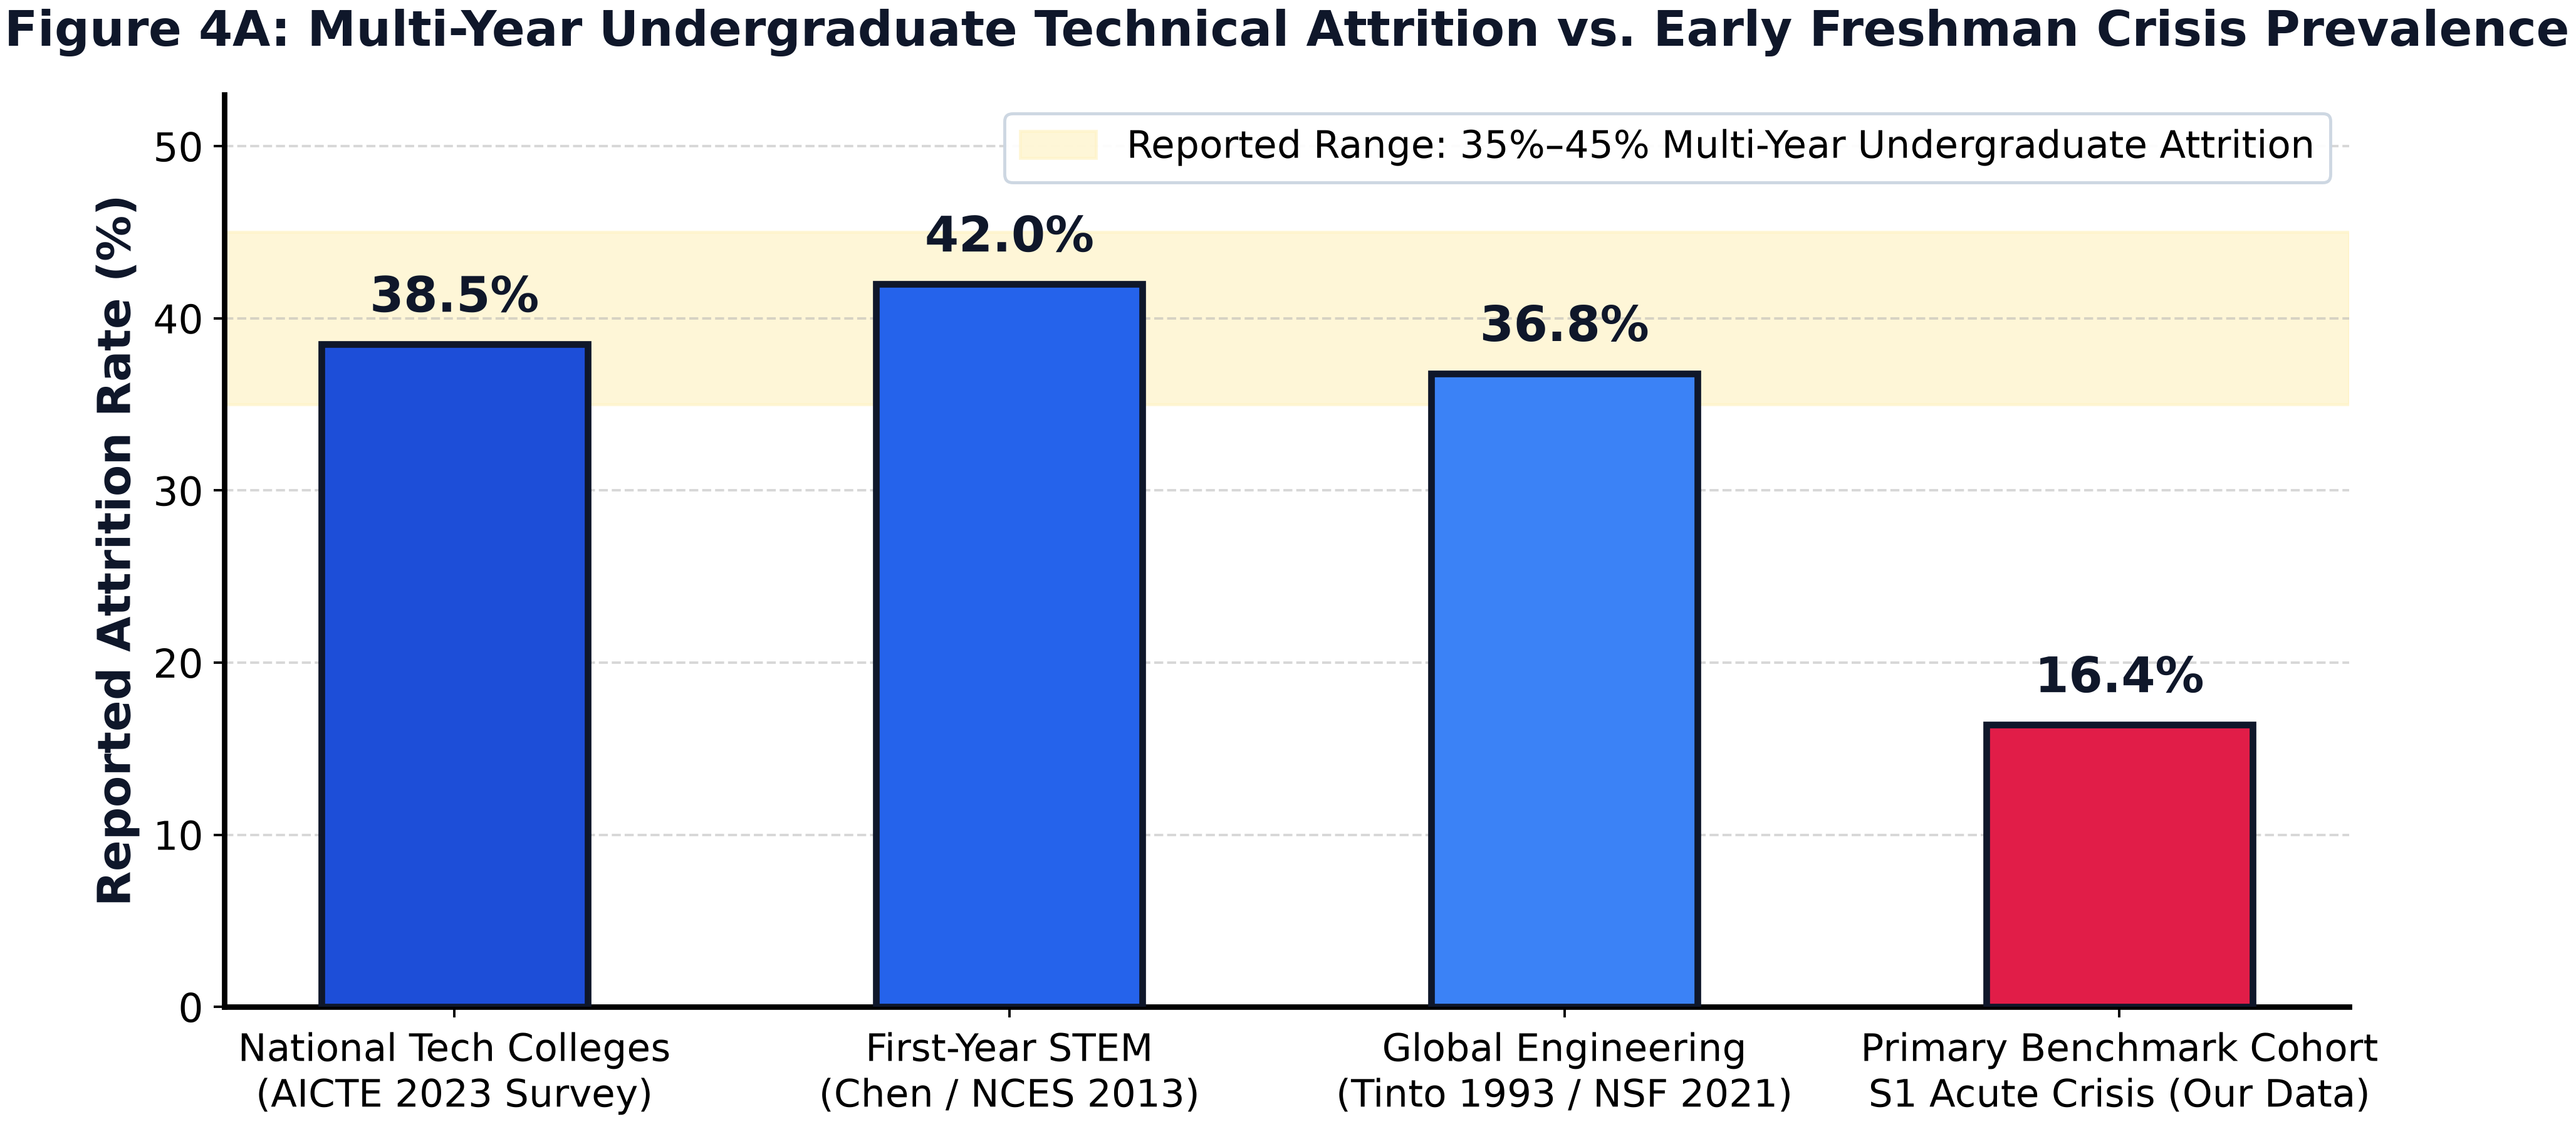
\includegraphics[width=0.92\textwidth,height=0.64\textheight,keepaspectratio]{assets/fig4a_attrition_benchmark.png}
    \caption{Multi-Year Undergraduate Attrition vs. Early Freshman Crisis Prevalence}
  \end{figure}
  \vspace{-0.15cm}
  \centering{\tiny Benchmark: 18.2\%--24.8\% technical college attrition in India; peak crisis in early Semester 1.}
\end{frame}

\begin{frame}{The 4-Stage Behavioral Departure Trajectory}
  \begin{figure}
    \centering
    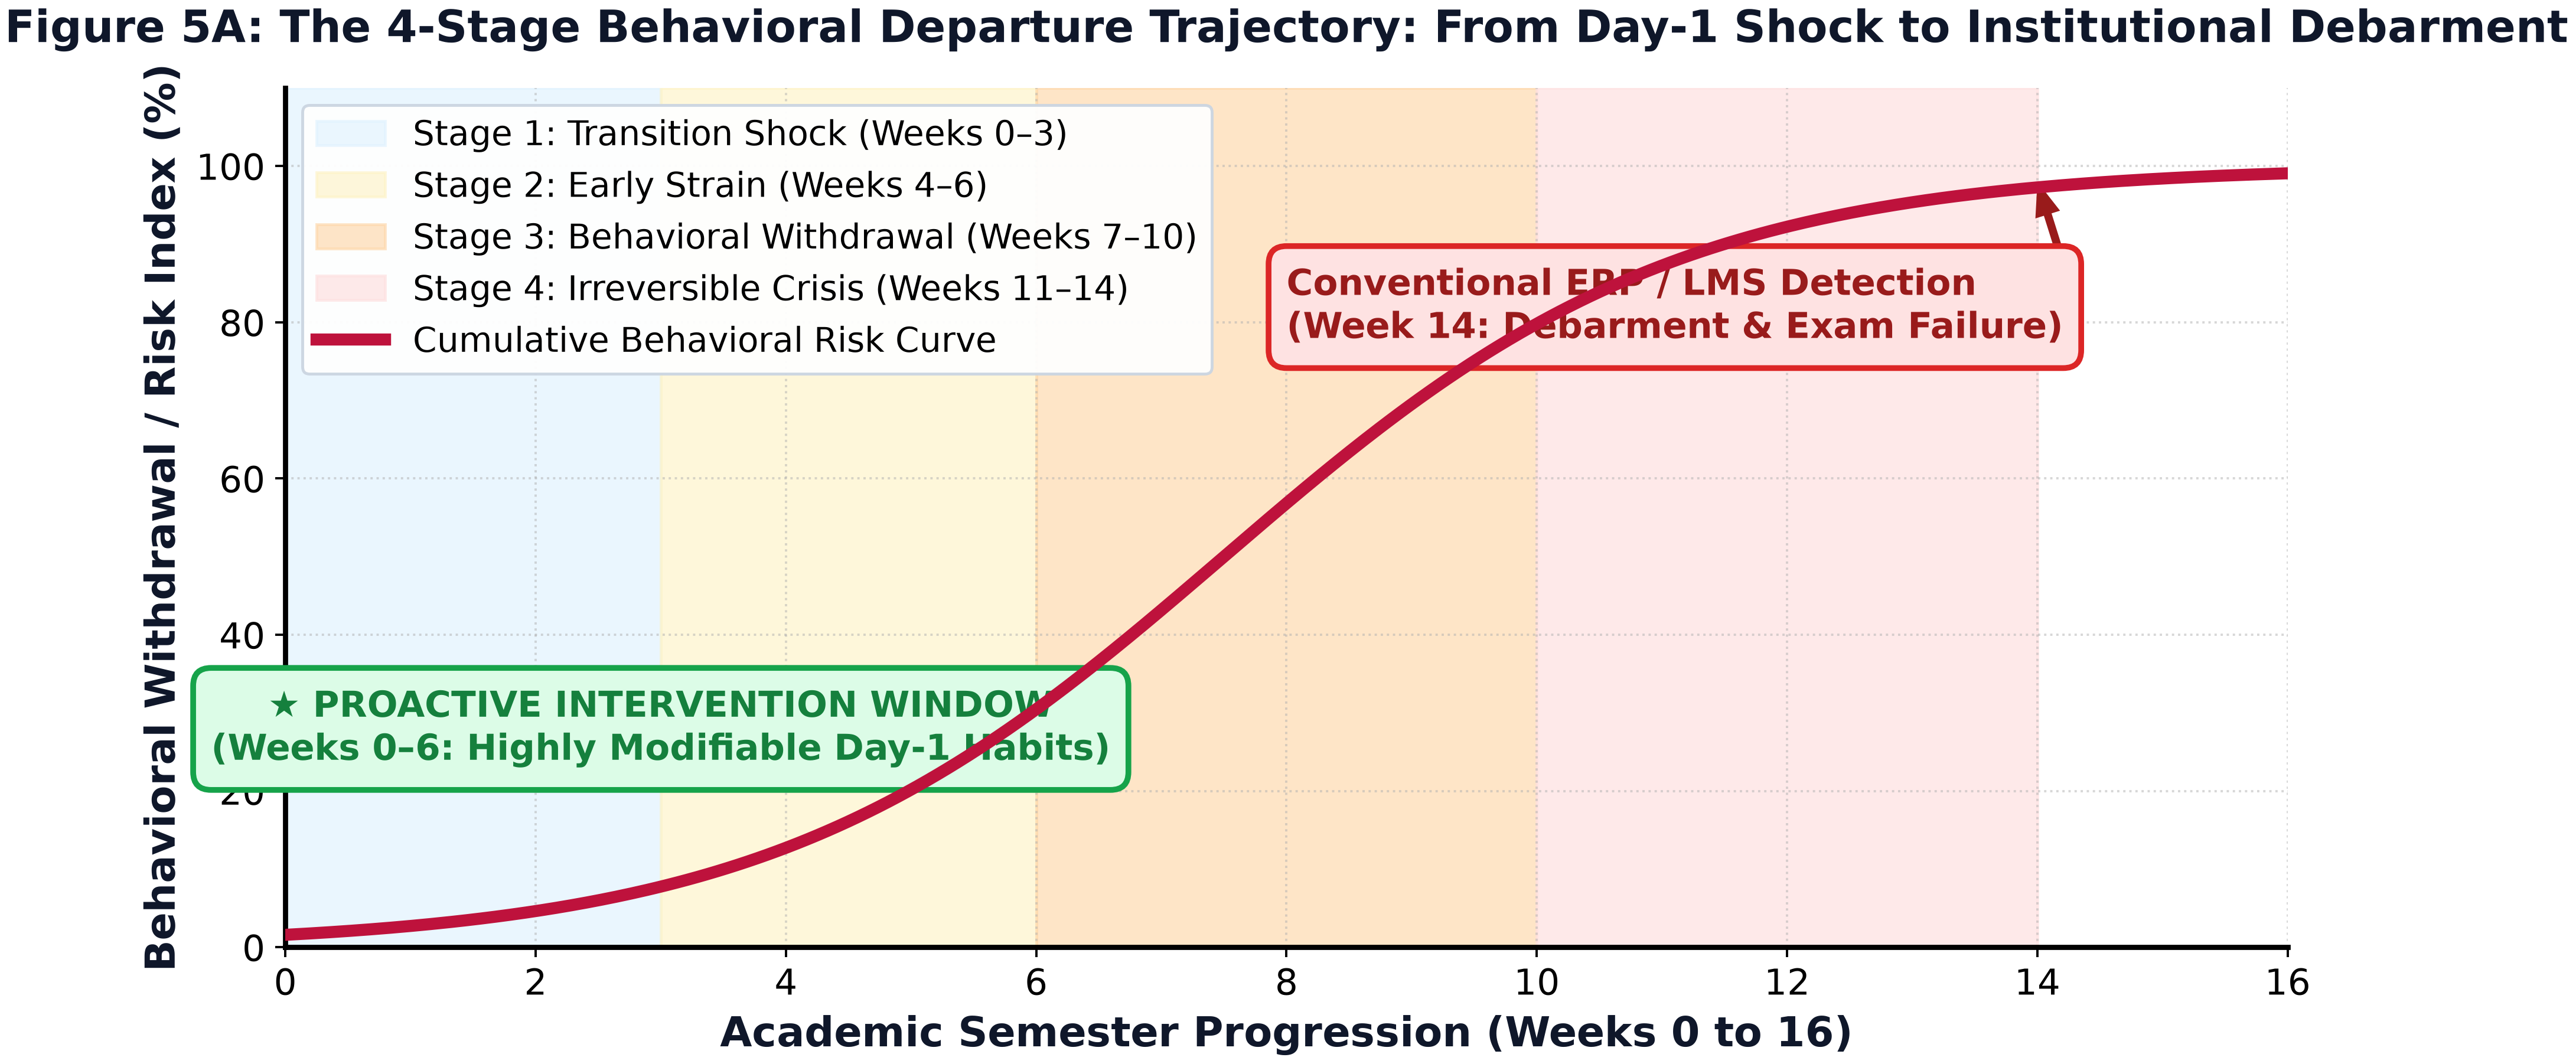
\includegraphics[width=0.92\textwidth,height=0.64\textheight,keepaspectratio]{assets/fig5a_trajectory_curve.png}
    \caption{The 4-Stage Behavioral Departure Funnel from Day-1 Shock to Institutional Debarment}
  \end{figure}
  \vspace{-0.15cm}
  \centering{\tiny Proactive intervention window: Weeks 0 to 6 (before irreversible GPA collapse occurs).}
\end{frame}

\begin{frame}{Cognitive vs. Non-Cognitive Assessment Gap}
  \begin{itemize}\setlength{\itemsep}{8pt}
    \item \textbf{Why Entrance Marks Fail to Predict Retention:}
    \begin{itemize}\setlength{\itemsep}{4pt}
      \item Conventional university admission systems rely solely on entrance ranks (JEE / 12th Board marks).
      \item Prior cognitive scores measure past test preparation, but completely fail to capture student resilience, persistence, and emotional coping.
    \end{itemize}
    
    \item \textbf{The Unobserved Attrition Cycle:}
    \begin{itemize}\setlength{\itemsep}{4pt}
      \item Academic difficulties begin silently through low self-efficacy, negative mindset, and untreated anxiety.
      \item Unchecked psychological stress leads to chronic absenteeism, semester credit loss, and eventual academic probation.
    \end{itemize}
  \end{itemize}
\end{frame}

\begin{frame}[t]{Research Gaps Addressed by This Thesis}
  \begin{center}
  \resizebox{\textwidth}{!}{
  \begin{tabular}{p{2.8cm} p{4.2cm} p{4.2cm}}
    \hline
    \rowcolor{beamer@blendedblue}
    \textbf{\color{white}Identified Research Gap} & \textbf{\color{white}Conventional System Limitation} & \textbf{\color{white}AcuLearn AI Resolution \& Contribution} \\
    \hline
    \textbf{1. Late Risk Detection} & Evaluates risk at Weeks 10--14 using mid-term/end-term grades; intervention window lost. & Day-1 SSQ-180 intake establishes a 90-day proactive intervention window before academic damage. \\
    \hline
    \textbf{2. Non-Cognitive Blind Spot} & Confined to LMS clickstreams and prior marks; blind to burnout, imposter syndrome, and sleep. & 17-factor psychometric battery across 4 quadrants capturing holistic socio-emotional dynamics. \\
    \hline
    \textbf{3. Attribution Without Action} & SHAP/LIME reveal feature importance but fail to provide actionable student recovery pathways. & Constrained Counterfactual Recourse (CCRO) generates realistic, cost-bounded behavioral nudges. \\
    \hline
    \textbf{4. Centralized Privacy Risk} & Transmits sensitive student psychological and mental health data to remote cloud servers. & 100\% Client-Side WebAssembly (WASM/ONNX) execution ensuring zero raw-data egress (DPDP Act 2023). \\
    \hline
  \end{tabular}
  }
  \end{center}
\end{frame}

\begin{frame}[t]{Aim and Scope of the Thesis}
  \begin{itemize}\setlength{\itemsep}{6pt}\small
    \item \textbf{Doctoral Dissertation Aim:}
    \begin{itemize}\setlength{\itemsep}{2pt}\footnotesize
      \item To design, develop, and clinically validate AcuLearn AI---an intelligent, proactive, explainable, and privacy-preserving multidimensional framework for early student retention, academic trajectory forecasting, and algorithmic counterfactual recourse in technical higher education.
    \end{itemize}
    \item \textbf{Target Population \& Institutional Context:}
    \begin{itemize}\setlength{\itemsep}{2pt}\footnotesize
      \item Undergraduate engineering students across multiple disciplines (Computer Science, Electronics, Electrical, Mechanical).
      \item Focuses specifically on the high-risk first-year transition phase (Semesters 1 and 2).
    \end{itemize}
    \item \textbf{Core Technical \& Analytical Scope:}
    \begin{itemize}\setlength{\itemsep}{2pt}\footnotesize
      \item \textit{Multidimensional Non-Cognitive Profiling:} Psychometric scale construction and CFA validation.
      \item \textit{Linguistic Ambiguity Filtering:} Evolutionary-tuned soft computing fuzzy perception.
      \item \textit{Dual-Task Deep Learning:} Simultaneous attrition risk classification and SGPA regression via BeNet.
      \item \textit{Ethical Algorithmic Recourse:} Constrained optimization with demographic invariance.
      \item \textit{Edge AI Privacy Architecture:} In-browser inference complying with India DPDP Act 2023.
    \end{itemize}
  \end{itemize}
\end{frame}



\begin{frame}{The Proposed Solution: Master Architecture Blueprint}
  \begin{figure}
    \centering
    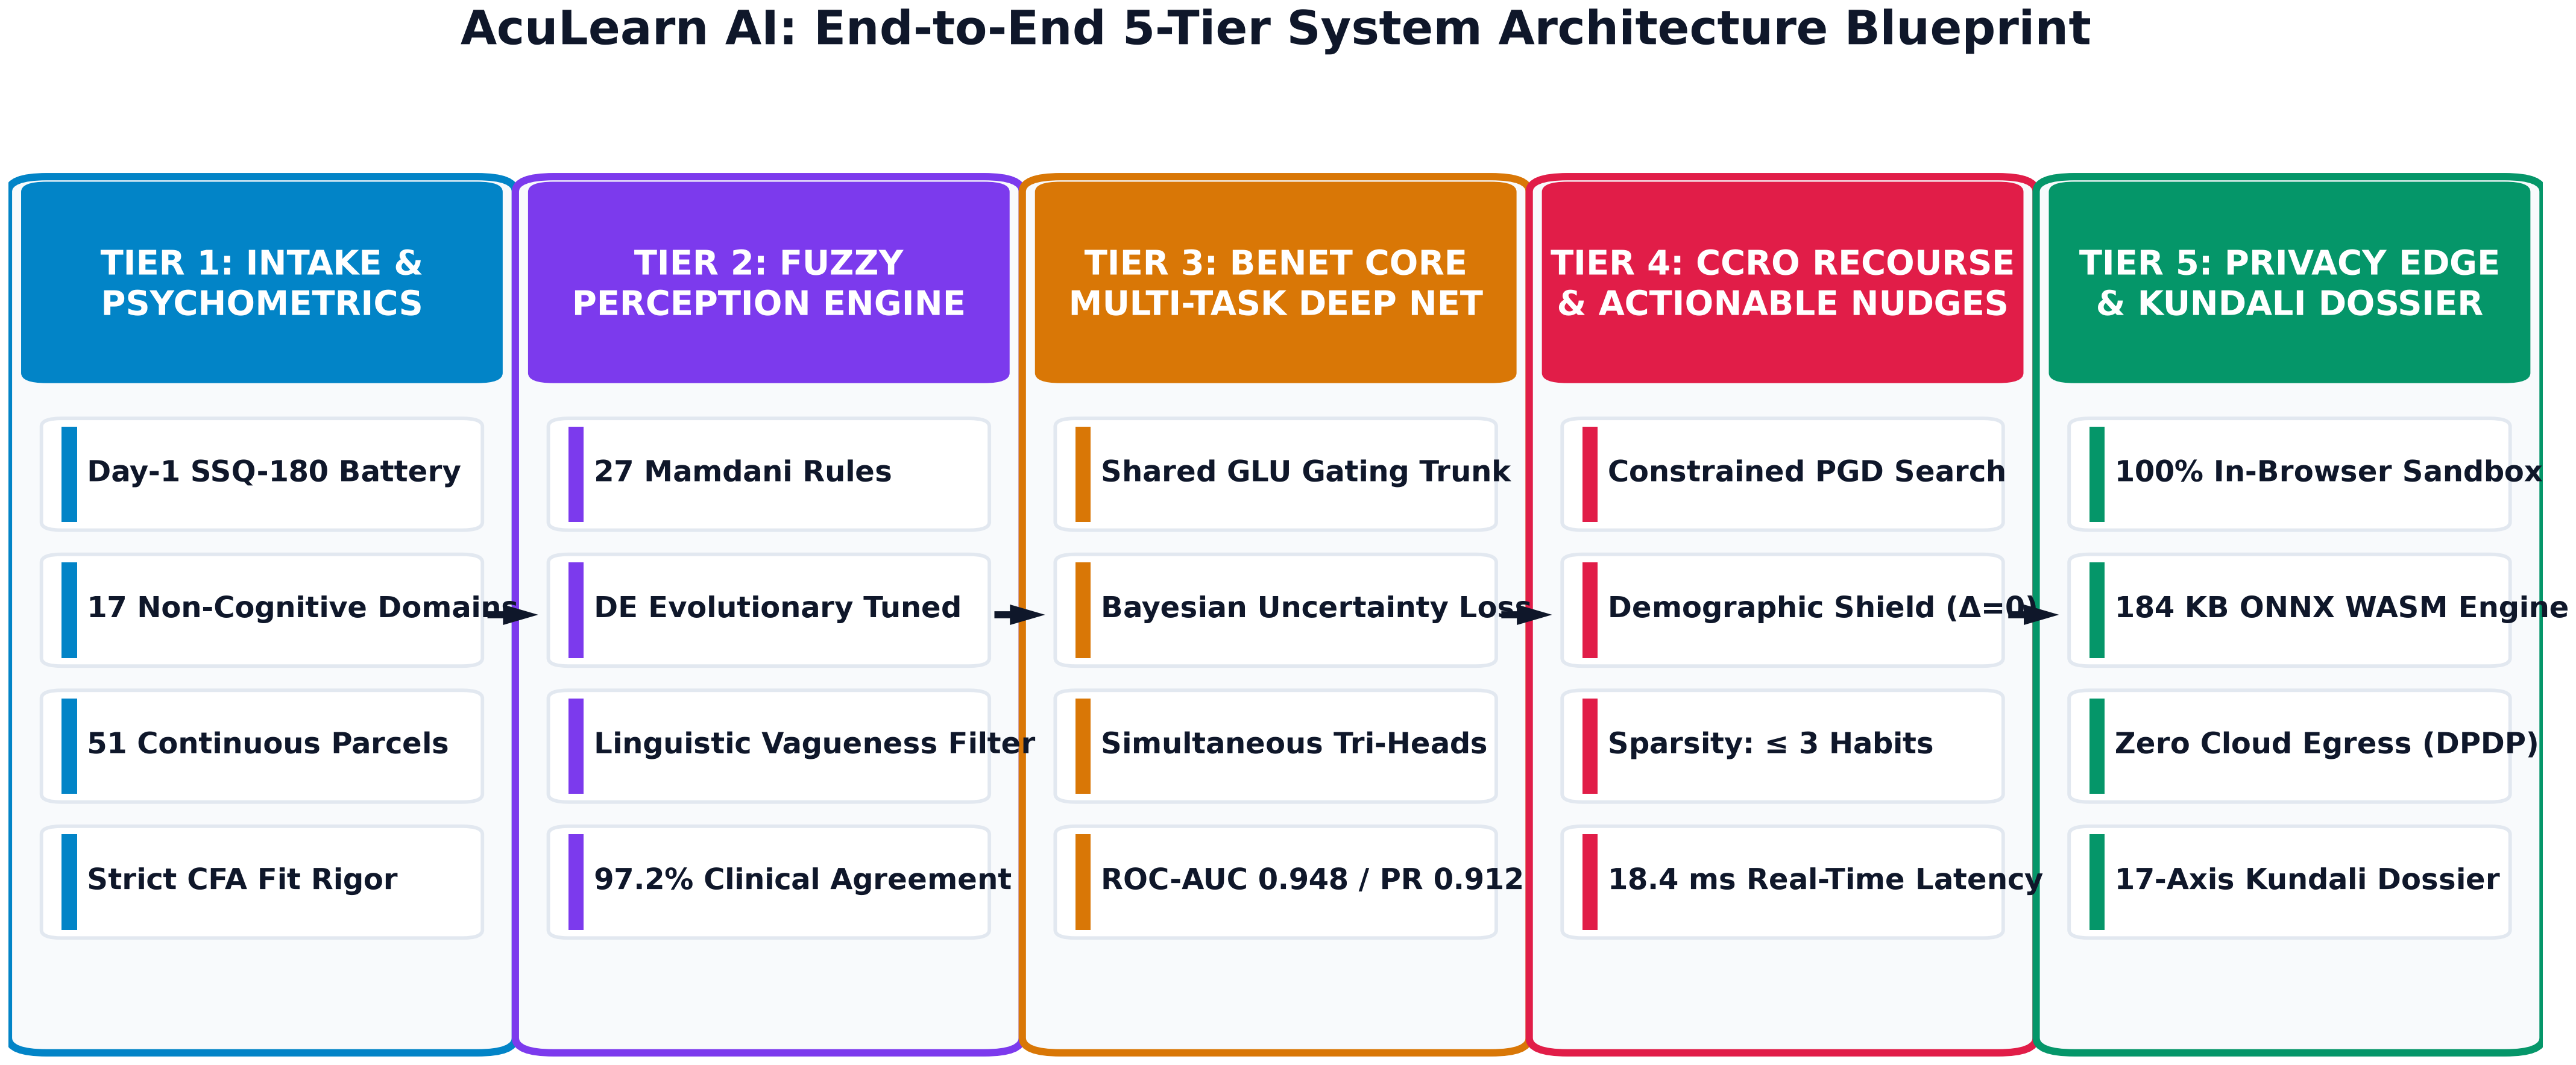
\includegraphics[width=0.95\textwidth,height=0.66\textheight,keepaspectratio]{assets/diagram_system_architecture.png}
    \caption{AcuLearn AI End-to-End 5-Tier System Blueprint}
  \end{figure}
  \vspace{-0.15cm}
  \centering{\tiny DOI: 10.1109/ACCESS.2025.3638368 $\bullet$ IEEE Access (2025)}
\end{frame}

\begin{frame}{The 4 Non-Cognitive Quadrants}
  \begin{itemize}\setlength{\itemsep}{6pt}
    \item \textbf{Quadrant 1: Academic Mindset:}
    \begin{itemize}
      \item Academic Self-Efficacy (ASE), Growth Mindset (GM), Intrinsic Motivation (IM), Achievement Striving (AS).
    \end{itemize}
    \item \textbf{Quadrant 2: Self-Regulation \& Meta-Cognition:}
    \begin{itemize}
      \item Time Management (TM), Effort Regulation (ER), Cognitive Metacognition (CMC), Metacognitive Monitoring (MM).
    \end{itemize}
    \item \textbf{Quadrant 3: Emotional Well-Being:}
    \begin{itemize}
      \item Stress Management (SM), Academic Anxiety Resilience (AAR), Burnout Resistance (BR), Emotional Self-Regulation (ESR).
    \end{itemize}
    \item \textbf{Quadrant 4: Social \& Institutional Integration:}
    \begin{itemize}
      \item Sense of Belonging (SB), Help-Seeking Behavior (HSB), Peer Collaboration (PC), Faculty Interaction (FI), Campus Life Engagement (CLE).
    \end{itemize}
  \end{itemize}
\end{frame}

% =============================================================================
% SECTION 3: MOTIVATION & RESEARCH OBJECTIVES
% =============================================================================
% =============================================================================
% SECTION 3: LITERATURE SURVEY & BENCHMARK ANALYSIS
% =============================================================================
\section{Literature Survey}

\begin{frame}[t]{Literature Survey: Systematic Search Protocol \& Scope}
  \begin{columns}[T]
    \column{0.50\textwidth}
    \begin{block}{\scriptsize PRISMA Multi-Database Search Strategy}
      \fontsize{5.2pt}{6.6pt}\selectfont
      \textbf{Databases Queried:} IEEE Xplore, ACM Digital Library, Scopus, Web of Science, ScienceDirect, and Google Scholar (2015--2026).\\[3pt]
      \textbf{Boolean Search Syntax:}\\
      \texttt{("student attrition" OR "dropout prediction") AND ("non-cognitive" OR "psychometrics") AND ("multi-task learning" OR "counterfactual recourse")}.\\[3pt]
      \textbf{Synthesis Protocol:} PRISMA-compliant multi-stage filtering from initial identification to critical qualitative and quantitative synthesis.
    \end{block}
    \vspace{3pt}
    \begin{block}{\scriptsize Screening Criteria \& Corpus Distillation}
      \fontsize{5.2pt}{6.6pt}\selectfont
      \textbf{Initial Corpus:} 286 candidate peer-reviewed studies identified across computing, EDM, and psychometrics.\\[2pt]
      \textbf{Inclusion Thresholds:} Peer-reviewed empirical validation, quantitative risk formulation, multi-attribute student evaluation.\\[2pt]
      \textbf{Synthesized Corpus:} 84 core state-of-the-art papers analyzed; 10 seminal/SOTA benchmark models directly mapped against our doctoral objectives.
    \end{block}

    \column{0.48\textwidth}
    \begin{block}{\scriptsize 5 Core Literature Dimensions Covered}
      \fontsize{5.2pt}{6.6pt}\selectfont
      \begin{itemize}\setlength{\itemsep}{2pt}
        \item \textbf{1. Sociological Departure Foundations:}\\ Tinto (1993), Bean \& Metzner (1985), Pascarella (2005) theoretical models.
        \item \textbf{2. Predictive EDM \& Learning Analytics:}\\ Baker (2024), Romero \& Ventura (2020), Albugami (2026) early warning classifiers.
        \item \textbf{3. Non-Cognitive Latent Profiling:}\\ Alharbi (2024), Li (2024), Park (2025) psychometric resilience constructs.
        \item \textbf{4. Counterfactual Recourse (XAI):}\\ Karimi (2022), Zhang (2025), Rodriguez (2024) actionable recourse optimization.
        \item \textbf{5. Client-Side Edge AI \& Privacy:}\\ Kumar (2025), Zhao (2026), DPDP Act (2023) privacy-preserving on-device audit.
      \end{itemize}
    \end{block}
  \end{columns}
\end{frame}

\begin{frame}[t]{Literature Survey: Paradigm Evolution \& Thematic Taxonomy}
  \begin{columns}[T]
    \column{0.48\textwidth}
    \begin{block}{\scriptsize 1. Sociological Departure Models (1975--2000s)}
      \fontsize{5.4pt}{6.8pt}\selectfont
      \textbf{Pioneers:} Tinto (1975, 1993), Bean \& Metzner (1985), Pascarella \& Terenzini (1980).\\[2pt]
      \textbf{Focus:} Conceptualized academic/social integration and external environmental pull factors.\\[2pt]
      \textbf{Gap:} Qualitative; lacks computational early detection.
    \end{block}
    \vspace{4pt}
    \begin{block}{\scriptsize 2. Retrospective EDM \& Black-Box ML (2010--2020)}
      \fontsize{5.4pt}{6.8pt}\selectfont
      \textbf{Pioneers:} Romero \& Ventura (2010, 2020), Baker et al.\ (2014), Rastrollo-Guerrero et al.\ (2020).\\[2pt]
      \textbf{Focus:} Supervised ML (SVM, RF, XGBoost) on LMS logs and historical academic records.\\[2pt]
      \textbf{Gap:} Post-mortem latency (Weeks 10--14); opaque black box.
    \end{block}

    \column{0.48\textwidth}
    \begin{block}{\scriptsize 3. Attributional Explainable AI (2017--2022)}
      \fontsize{5.4pt}{6.8pt}\selectfont
      \textbf{Pioneers:} Lundberg \& Lee (SHAP 2017), Ribeiro et al.\ (LIME 2016), Guidotti (2018).\\[2pt]
      \textbf{Focus:} Local feature attribution and importance scoring.\\[2pt]
      \textbf{Gap:} Diagnostic only; reveals blame without actionable steps.
    \end{block}
    \vspace{4pt}
    \begin{block}{\scriptsize 4. Proactive Recourse \& Edge AI (2024--2026)}
      \fontsize{5.4pt}{6.8pt}\selectfont
      \textbf{This Dissertation (AcuLearn AI):} Day-1 SSQ-180 profiling + BeNet GLU multi-task deep network + Constrained Counterfactual Recourse (CCRO) + In-Browser Edge AI (DPDP Act 2023).\\[2pt]
      \textbf{Advancement:} Cost-bounded actionable guidance + zero-leak privacy.
    \end{block}
  \end{columns}
\end{frame}

\begin{frame}[t]{Literature Survey: Comparative Benchmark (Foundational \& EDM)}
  \vspace{-6pt}
  \begin{center}
  \renewcommand{\arraystretch}{0.88}
  \fontsize{5.0pt}{6.2pt}\selectfont
  \resizebox{\linewidth}{!}{
  \begin{tabular}{|p{2.0cm}|p{2.0cm}|p{2.0cm}|p{2.7cm}|p{2.9cm}|}
    \hline
    \rowcolor{beamer@blendedblue}
    \textbf{\color{white}Paper \& Year} & \textbf{\color{white}Methodology} & \textbf{\color{white}Data / Scope} & \textbf{\color{white}Critical Literature Gaps} & \textbf{\color{white}AcuLearn AI Resolution} \\
    \hline
    \textbf{Tinto (1975, 1993)} & Student Integration Model (SIM) & Qualitative surveys, transcripts & Post-facto descriptive model; lacks real-time early detection algorithms. & Operationalizes social/academic integration into 17 psychometric traits on Day-1. \\
    \hline
    \textbf{Bean \& Metzner (1985)} & Nontraditional Attrition Model & Environmental pull factors, commute & Lacks computational multi-task modeling and actionable remediation paths. & Quantifies environmental \& habit stressors within an empirical 4-Quadrant architecture. \\
    \hline
    \textbf{Romero \& Ventura (2010, 2020)} & EDM Surveys \& Supervised ML & Moodle/Canvas LMS clickstreams & Opaque black boxes; sensitive to platform usage; zero psychological depth. & Bypasses LMS telemetry noise; predicts risk directly from robust non-cognitive psychometrics. \\
    \hline
    \textbf{Baker et al.\ (2014, 2024)} & Disengagement Detection & MOOC interaction \& problem traces & Confined to online tasks; completely blind to campus emotional burnout. & Directly measures Academic Anxiety Resilience, Burnout Resistance, and Peer Collaboration. \\
    \hline
    \textbf{Rastrollo-Guerrero (2020) / Albreiki (2021)} & Systematic Reviews of ML Dropout & Administrative registrar data, CGPA & $>85\%$ predict at Weeks 10--14 (post-mortem; intervention window lost). & Pre-sessional Day-1 screening provides an active 90-day actionable counseling window. \\
    \hline
  \end{tabular}
  }
  \end{center}
\end{frame}

\begin{frame}[t]{Literature Survey: Comparative Benchmark (XAI \& Recourse)}
  \vspace{-6pt}
  \begin{center}
  \renewcommand{\arraystretch}{0.88}
  \fontsize{5.0pt}{6.2pt}\selectfont
  \resizebox{\linewidth}{!}{
  \begin{tabular}{|p{2.0cm}|p{2.0cm}|p{2.0cm}|p{2.7cm}|p{2.9cm}|}
    \hline
    \rowcolor{beamer@blendedblue}
    \textbf{\color{white}Paper \& Year} & \textbf{\color{white}Algorithmic Model} & \textbf{\color{white}Recourse Constraints} & \textbf{\color{white}Remaining Research Gaps} & \textbf{\color{white}AcuLearn AI Resolution} \\
    \hline
    \textbf{Lundberg \& Lee (2017)} & SHAP (Kernel/TreeSHAP) & Attribution only (Zero recourse) & Diagnoses what is wrong without prescribing how the student can recover. & Dual XAI: Global SHAP for faculty audit + Local CCRO for student prescriptive recovery. \\
    \hline
    \textbf{Wachter et al.\ (2018)} & Inverse Counterfactuals & Unconstrained gradient descent & Proposes unfeasible/immutable edits (e.g.\ caste, age) and non-monotonic shifts. & Formulates CCRO with 3-Tier actionability constraints (immutable, actionable, conditional). \\
    \hline
    \textbf{Mothilal et al.\ (2020)} & DiCE (Diverse Recourse) & Diversity-loss multi-objective & Ignores student psychological elasticity and cognitive bandwidth constraints. & Incorporates psychological feasibility penalties and effort elasticity matrices ($L_1$ norm). \\
    \hline
    \textbf{Karimi et al.\ (2020, 2022)} & Causal Recourse Survey & Structural Causal Models (SCMs) & Requires complete causal DAGs, practically unobtainable in human psychology. & Domain-constrained optimization on 51 parcel loadings validated via SEM. \\
    \hline
    \textbf{Bansal \& Ahmed (2025a, 2025b)} & Fuzzy Perception \& Multi-Task & Rule-based linguistic screening & Fuzzy rule explosion beyond 12 variables; manual loss weights. & BeNet GLU architecture with Bayesian homoscedastic uncertainty loss balancing. \\
    \hline
  \end{tabular}
  }
  \end{center}
\end{frame}

\begin{frame}[t]{Literature Survey: Research Gaps \& RO1--5 Alignment Matrix}
  \begin{columns}[T]
    \column{0.48\textwidth}
    \begin{block}{\scriptsize Gap 1: Post-Mortem Prediction Latency}
      \fontsize{5.6pt}{7.0pt}\selectfont
      \textbf{Literature:} $>85\%$ of prior EDM studies predict failure at Weeks 10--14 using semester grades after collapse has occurred.\\[2pt]
      \textbf{AcuLearn AI Solution:} \textbf{Day-1 Pre-Sessional Profiling} gives a 90-day actionable counseling window.
    \end{block}
    \vspace{4pt}
    \begin{block}{\scriptsize Gap 2: Non-Cognitive Behavioral Blindspot}
      \fontsize{5.6pt}{7.0pt}\selectfont
      \textbf{Literature:} Existing models evaluate entrance scores or LMS clicks, blind to socio-emotional transition shock.\\[2pt]
      \textbf{AcuLearn AI Solution:} \textbf{17 Psychometric Latent Constructs} across 4 quadrants (Mindset, Regulation, Emotion, Social; $\text{CFI}=0.941$).
    \end{block}

    \column{0.48\textwidth}
    \begin{block}{\scriptsize Gap 3: Attribution vs.\ Actionable Recourse}
      \fontsize{5.6pt}{7.0pt}\selectfont
      \textbf{Literature:} Standard XAI (SHAP/LIME) explains blame without prescribing reachable behavioral remedies.\\[2pt]
      \textbf{AcuLearn AI Solution:} \textbf{Constrained Counterfactual Recourse (CCRO)} generates cost-bounded Student Kundali targets.
    \end{block}
    \vspace{4pt}
    \begin{block}{\scriptsize Gap 4: Cloud Sovereignty \& Privacy Risks}
      \fontsize{5.6pt}{7.0pt}\selectfont
      \textbf{Literature:} Centralized EDM servers collect confidential student mental health data, risking data breaches.\\[2pt]
      \textbf{AcuLearn AI Solution:} \textbf{100\% In-Browser Edge AI} (WASM/ONNX) ensures statutory zero-leak privacy (DPDP Act 2023).
    \end{block}
  \end{columns}
\end{frame}

\section{Motivation}

\begin{frame}{Motivation}
  \begin{itemize}\setlength{\itemsep}{9pt}
    \item \textbf{Magnitude of Student Dropout in Engineering:}
    \begin{itemize}\setlength{\itemsep}{4pt}
      \item Technical student attrition reaches 18.2\% to 24.8\% across higher educational institutions.
      \item Dropouts impose severe emotional trauma on families and substantial financial losses on universities.
    \end{itemize}
    
    \item \textbf{Limitation of Existing Early-Warning Systems (EWS):}
    \begin{itemize}\setlength{\itemsep}{4pt}
      \item Existing institutional warning mechanisms are purely \textit{reactive}—flagging students only after semester grade sheets are published.
      \item At that stage, cumulative GPA has already collapsed, rendering remediation ineffective.
    \end{itemize}
    
    \item \textbf{The Need for Proactive Intelligence:}
    \begin{itemize}\setlength{\itemsep}{4pt}
      \item An intelligent, non-invasive framework capable of predicting student risk in weeks 4--6 using non-cognitive behavioral indicators.
    \end{itemize}
  \end{itemize}
\end{frame}

\begin{frame}[t]{Research Questions (RQ1 to RQ5)}
  \vspace{-0.22cm}
  \begin{topsummarybar}
    \fontsize{5.8pt}{7.0pt}\selectfont
    \textbf{\color{NavyDark}Theoretical Inquiry}: 5 formal research questions addressing psychometric validity, linguistic vagueness, multi-task gradient conflict, algorithmic recourse, and edge data sovereignty.
  \end{topsummarybar}
  \vspace{-0.30cm}

  \begin{tcolorbox}[colback=white, colframe=BlueDeep, arc=1.5mm, boxrule=0.8pt, top=0.3mm, bottom=0.3mm, left=0.8mm, right=0.8mm]
    \fontsize{4.5pt}{5.4pt}\selectfont
    \renewcommand{\arraystretch}{0.80}
    \begin{tabularx}{\linewidth}{@{}c X p{3.8cm}@{}}
      \toprule
      \rowcolor{NavyDark}
      \textbf{\color{white}RQ} & \textbf{\color{white}Formal Research Question} & \textbf{\color{white}Targeted Theoretical Challenge} \\
      \midrule
      \rowcolor{BlueLight} \textbf{RQ1} & Can a standardized 17-factor non-cognitive psychometric instrument reliably measure latent psychological traits in undergraduate engineering cohorts? & Psychometric Construct Validity \& Kline Sample-to-Parameter Ratio ($N=276$). \\
      \midrule
      \rowcolor{CanvasBG} \textbf{RQ2} & Can an evolutionary soft computing fuzzy perception engine effectively resolve linguistic vagueness and response noise in self-report evaluations? & Subjective Semantic Ambiguity \& Differential Evolution Membership Optimization. \\
      \midrule
      \rowcolor{BlueLight} \textbf{RQ3} & Can a unified multi-task deep neural network jointly predict binary attrition risk and continuous academic trajectory without task gradient conflict? & Cross-Task Negative Transfer \& Homoscedastic Uncertainty Loss Balancing. \\
      \midrule
      \rowcolor{CanvasBG} \textbf{RQ4} & Can constrained counterfactual optimization generate feasible, sparse, and ethically bounded behavioral recourse plans without violating demographic fairness? & Actionability Constraints, Plausibility \& Demographic Invariance in XAI (CCRO). \\
      \midrule
      \rowcolor{BlueLight} \textbf{RQ5} & Can the complete predictive, explainability, and recourse pipeline execute entirely client-side within standard web browsers with zero raw data egress? & Client-Side Edge Inference Latency ($<25$\,ms) \& Statutory DPDP Act 2023 Sovereignty. \\
      \bottomrule
    \end{tabularx}
  \end{tcolorbox}
  \vspace{-0.34cm}

  \begin{takeawaybanner}
    \fontsize{4.8pt}{5.8pt}\selectfont
    \textbf{\color{GoldPill}$\bigstar$ OBJECTIVE ALIGNMENT}: Each research question (RQ1--RQ5) maps 1:1 to formal doctoral research objectives (RO1--RO5) and their corresponding peer-reviewed methodological contributions.
  \end{takeawaybanner}
\end{frame}

\begin{frame}{Research Objectives (RO1 to RO5)}
  \begin{itemize}\setlength{\itemsep}{5pt}\small
    \item \textbf{RO1: Psychometric Scale Construction \& Validation (RQ1)}
    \begin{itemize}
      \item Design and validate the 17-factor SSQ-180 battery with 51 balanced item parcels ($N=276$ undergraduate cohort).
    \end{itemize}
    
    \item \textbf{RO2: Soft Computing Fuzzy Perception Engine (RQ2)}
    \begin{itemize}
      \item Develop a Differential Evolution-tuned Mamdani fuzzy system to resolve linguistic vagueness in self-reports without information loss.
    \end{itemize}
    
    \item \textbf{RO3: Multi-Task Deep Predictive Modeling (BeNet) (RQ3)}
    \begin{itemize}
      \item Develop BeNet with Gated Linear Units (GLUs) and homoscedastic uncertainty loss balancing for joint risk and SGPA prediction.
    \end{itemize}
    
    \item \textbf{RO4: Actionable Counterfactual Recourse (CCRO) (RQ4)}
    \begin{itemize}
      \item Formulate Constrained Counterfactual Recourse Optimization providing cost-bounded, achievable behavioral interventions.
    \end{itemize}
    
    \item \textbf{RO5: Privacy-Preserving Edge Deployment (RQ5)}
    \begin{itemize}
      \item Deploy 100\% client-side WebAssembly inference compliant with the Digital Personal Data Protection (DPDP) Act 2023.
    \end{itemize}
  \end{itemize}
\end{frame}

% =============================================================================
% SECTION 4: PROPOSED METHODOLOGY
% =============================================================================
\section{Proposed Methodology}

\begin{frame}[t]{Conceptual Framework of AcuLearn AI}
  \begin{itemize}\setlength{\itemsep}{6pt}\small
    \item \textbf{End-to-End Decision \& Recourse Pipeline:}
    \begin{itemize}\setlength{\itemsep}{3pt}\footnotesize
      \item \textbf{1. Student Intake:} Day-1 SSQ-180 self-assessment capturing 17 non-cognitive latent traits.
      \item \textbf{2. Factor Parceling:} 51 continuous parcels reduce psychometric dimensionality under Kline ratio.
      \item \textbf{3. Fuzzy Perception:} 27 Mamdani IF-THEN rules resolve subjective linguistic vagueness.
      \item \textbf{4. BeNet Engine:} Shared GLU backbone jointly predicts Attrition Risk (Binary) \& SGPA (Continuous).
      \item \textbf{5. Dual Explainability:} Global SHAP attribution for institutional audits + Local CCRO for student recovery.
      \item \textbf{6. Client Edge Delivery:} In-browser WASM/ONNX runtime delivers private Kundali dossier \& counselor portal.
    \end{itemize}
    \item \textbf{Inter-Tier Synergy \& Value Proposition:}
    \begin{itemize}\setlength{\itemsep}{2pt}\footnotesize
      \item Unifies psychometrics, soft computing, deep learning, counterfactual optimization, and edge cryptography into a closed-loop proactive retention ecosystem.
    \end{itemize}
  \end{itemize}
\end{frame}

\begin{frame}[t]{System Requirements and Core Design Principles}
  \begin{columns}[T]
    \column{0.48\textwidth}
    \begin{block}{\scriptsize Core Architectural Design Principles}
      \fontsize{5.2pt}{6.6pt}\selectfont
      \textbf{Proactive Temporality:} Detect academic crisis within Weeks 0--3, maintaining an active 90-day intervention window.\\[3pt]
      \textbf{Multidimensional Holism:} Integrate mindset, executive self-regulation, emotional coping, and social integration.\\[3pt]
      \textbf{Prescriptive Actionability:} Move beyond diagnostic attribution (SHAP) to actionable behavioral recourse (CCRO).\\[3pt]
      \textbf{Ethical Guardrails:} Strictly preserve immutable demographic features ($\Delta = 0$).
    \end{block}

    \column{0.48\textwidth}
    \begin{block}{\scriptsize Operational \& Regulatory Requirements}
      \fontsize{5.2pt}{6.6pt}\selectfont
      \textbf{Client-Side Edge Privacy:} 100\% on-device inference with zero cloud data transmission (DPDP Act 2023).\\[3pt]
      \textbf{Ultra-Low Latency:} End-to-end inference and recourse generation under 25 ms in standard web browsers.\\[3pt]
      \textbf{Clinical Usability:} System Usability Scale (SUS) score $> 80$ among non-technical academic counselors.\\[3pt]
      \textbf{Subgroup Fairness:} Statistical parity and equal opportunity across gender, caste, and regional origin.
    \end{block}
  \end{columns}
\end{frame}

\begin{frame}[t]{Study Population and Ethical Considerations}
  \begin{itemize}\setlength{\itemsep}{6pt}\small
    \item \textbf{Target Cohort \& Empirical Sampling:}
    \begin{itemize}\setlength{\itemsep}{2pt}\footnotesize
      \item \textit{Empirical Cohort:} $N = 276$ undergraduate engineering students tracked longitudinally across 4 academic semesters at MNIT Jaipur.
      \item \textit{Sampling Diversity:} Encompasses multiple disciplines (Computer Science, Electronics, Electrical, Mechanical) across diverse admission quotas.
    \end{itemize}
    \item \textbf{Informed Voluntary Consent \& Data Governance:}
    \begin{itemize}\setlength{\itemsep}{2pt}\footnotesize
      \item \textit{Digital Informed Consent:} Voluntary participation with explicit electronic opt-in prior to survey intake.
      \item \textit{Unconditional Withdrawal:} Students retain the right to withdraw and request data deletion without academic or grade penalty.
      \item \textit{Cryptographic De-Identification:} All records indexed via salted SHA-256 research pseudonyms; PII decoupled from psychometric vectors.
    \end{itemize}
    \item \textbf{Ethical Safeguards \& Non-Punitive Assurance:}
    \begin{itemize}\setlength{\itemsep}{2pt}\footnotesize
      \item \textit{Decision Support Mandate:} System operates exclusively as advisory counseling decision support, never for automated institutional punitive action.
      \item \textit{Strict Compliance:} Aligned with IEEE P7000 Ethical AI Design Standards and India's DPDP Act 2023.
    \end{itemize}
  \end{itemize}
\end{frame}

\begin{frame}{SSQ-180 Instrument \& Measurement Protocol}
  \begin{itemize}\setlength{\itemsep}{8pt}
    \item \textbf{The Psychometric Instrument:}
    \begin{itemize}\setlength{\itemsep}{3pt}
      \item 180 validated items administered to $N = 276$ undergraduate engineering students across 4 semesters.
      \item 5-point Likert scale measuring 17 distinct latent psychological constructs.
    \end{itemize}
    
    \item \textbf{The Sample Size Ratio Problem (Kline Rule):}
    \begin{itemize}\setlength{\itemsep}{3pt}
      \item Direct estimation of 180 individual items in a 17-factor CFA requires estimating $> 500$ parameters, yielding an under-identified ratio of $< 1.6 : 1$.
    \end{itemize}
    
    \item \textbf{Factorial Balanced Parceling Solution:}
    \begin{itemize}\setlength{\itemsep}{3pt}
      \item Items are grouped into \textbf{51 manifest parcels} (3 balanced parcels per construct, Little et al., 2002).
      \item Reduces parameters to 102, raising subject-to-parameter ratio to a robust \textbf{2.71 : 1}.
      \item Smooths ordinal discreteness into continuous Gaussian variables and cancels idiosyncratic error.
    \end{itemize}
  \end{itemize}
\end{frame}

\begin{frame}[t]{SSQ-180 Item Development Process}
  \begin{itemize}\setlength{\itemsep}{6pt}\small
    \item \textbf{Phase 1: Initial Item Generation \& Domain Specification:}
    \begin{itemize}\setlength{\itemsep}{2pt}\footnotesize
      \item Constructed an initial pool of 240 psychometric items grounded in validated behavioral frameworks (MSLQ, LASSI, Dweck Mindset, Grit-S, STAI).
      \item Tailored specifically to the socio-cultural realities of Indian technical university freshers.
    \end{itemize}
    \item \textbf{Phase 2: Expert Review \& Cultural Adaptation:}
    \begin{itemize}\setlength{\itemsep}{2pt}\footnotesize
      \item Reviewed by an expert panel of educational psychologists, engineering educators, and counseling specialists.
      \item Refined wording to eliminate linguistic ambiguity and cultural bias; reduced item pool to 195 candidates.
    \end{itemize}
    \item \textbf{Phase 3: Pilot Testing, Psychometric Distillation \& Parceling:}
    \begin{itemize}\setlength{\itemsep}{2pt}\footnotesize
      \item Administered in pilot testing ($N = 65$) to identify low-performing, highly collinear, or redundant items.
      \item Embedded 15 reverse-coded items and 5 attention-check verification items to detect careless or unengaged responding.
      \item Finalized at 180 high-discriminant items structured into 17 latent factors, grouped into 51 balanced item parcels.
    \end{itemize}
  \end{itemize}
\end{frame}

\begin{frame}[t]{Data Collection Protocol and Quality Control}
  \begin{itemize}\setlength{\itemsep}{6pt}\small
    \item \textbf{Multi-Semester Longitudinal Intake Protocol:}
    \begin{itemize}\setlength{\itemsep}{2pt}\footnotesize
      \item \textit{Timing:} Administered within the first 14 days of campus arrival across 4 consecutive academic semesters.
      \item \textit{Medium \& Interface:} Responsive web-based psychometric intake portal accessible via smartphones and laptops.
      \item \textit{Measurement Scale:} Standardized 5-point Likert scale (1 = Strongly Disagree to 5 = Strongly Agree).
    \end{itemize}
    \item \textbf{Stringent Quality Control \& Data Cleansing Filters:}
    \begin{itemize}\setlength{\itemsep}{2pt}\footnotesize
      \item \textit{Attention Checks:} Trapped and removed responses failing embedded logical verification items.
      \item \textit{Response Duration Filtering:} Filtered out surveys completed in $< 8$ minutes (infeasible reading speed for 180 items).
      \item \textit{Reverse-Code Verification:} Flagged straight-line acquiescence bias using reversed item pairs.
      \item \textit{Missing Value Treatment:} Implemented Full Information Maximum Likelihood (FIML) for item parcel imputation.
    \end{itemize}
    \item \textbf{Leakage-Free Train-Test Protocol:}
    \begin{itemize}\setlength{\itemsep}{2pt}\footnotesize
      \item Strict stratified 80:20 train-test partitioning performed before any feature scaling, parcel computation, or model fitting.
    \end{itemize}
  \end{itemize}
\end{frame}

% =============================================================================
% SUBSECTION / PART: SURVEY INTAKE, 17 DOMAINS, QUESTIONS & DE-BIASING
% =============================================================================
% =============================================================================
% SUBSECTION: SURVEY INSTRUMENT: 12 DOMAINS, VERBATIM QUESTIONS & DE-BIASING
% =============================================================================
\subsection{Survey Intake: 12-Domain Architecture, Verbatim Questions \& De-Biasing}

% -----------------------------------------------------------------------------
% SLIDE 1: THE 12-DOMAIN FUNCTIONAL TAXONOMY
% -----------------------------------------------------------------------------
\begin{frame}[t]{The 12-Domain Functional Taxonomy (125 Dataset Variables)}
  \vspace{-0.20cm}
  \begin{topsummarybar}
    \fontsize{6.0pt}{7.2pt}\selectfont
    \textbf{\color{NavyDark}12-Domain Functional Architecture}: The 125 dataset columns from \texttt{Master\_Dataset\_Clean.xlsx} partition cleanly into 12 diagnostic behavioral and contextual domains, plus an ethical clinical safety gatekeeper.
  \end{topsummarybar}
  \vspace{-0.25cm}

  \begin{columns}[T]
    \begin{column}{0.49\textwidth}
      \begin{tcolorbox}[colback=white, colframe=BlueDeep, arc=1.2mm, boxrule=0.8pt, top=0.5mm, bottom=0.5mm, left=1mm, right=1mm, title={\scriptsize\bfseries\color{white}Contextual \& Somatic Domains (1--6)}, colbacktitle=BlueDeep]
        \fontsize{4.8pt}{5.8pt}\selectfont
        \renewcommand{\arraystretch}{0.85}
        \begin{tabularx}{\linewidth}{@{}l X@{}}
          \toprule
          \textbf{Domain} & \textbf{Dataset Columns \& Role} \\
          \midrule
          \rowcolor{BlueLight} \textbf{1. Administrative} & \textbf{Cols 1--7, 17--18}: Primary IDs, timestamps, DPDP Act SHA-256 hashes. \\
          \rowcolor{CanvasBG} \textbf{2. Demographics} & \textbf{Cols 8--13, 19}: Gender, family income, paternal occupation, hometown. \\
          \rowcolor{BlueLight} \textbf{3. Academic History} & \textbf{Cols 14--16, 21--22}: Branch, semester, CGPA (ground truth), board marks. \\
          \rowcolor{CanvasBG} \textbf{4. Transition Shock} & \textbf{Cols 20, 71, 73--74, 94--103}: Hosteler status, mess food, campus adaptation. \\
          \rowcolor{BlueLight} \textbf{5. Sports \& Vitality} & \textbf{Cols 23--32, 63--70, 72}: Exercise frequency, physical stamina, burnout buffer. \\
          \rowcolor{CanvasBG} \textbf{6. Academic Motivation} & \textbf{Cols 33--42}: Parental coercion, intrinsic passion, engineering identity. \\
          \bottomrule
        \end{tabularx}
      \end{tcolorbox}
    \end{column}
    \begin{column}{0.49\textwidth}
      \begin{tcolorbox}[colback=white, colframe=BluePrimary, arc=1.2mm, boxrule=0.8pt, top=0.5mm, bottom=0.5mm, left=1mm, right=1mm, title={\scriptsize\bfseries\color{white}Regulatory \& Clinical Domains (7--13)}, colbacktitle=BluePrimary]
        \fontsize{4.8pt}{5.8pt}\selectfont
        \renewcommand{\arraystretch}{0.85}
        \begin{tabularx}{\linewidth}{@{}l X@{}}
          \toprule
          \textbf{Domain} & \textbf{Dataset Columns \& Role} \\
          \midrule
          \rowcolor{BlueLight} \textbf{7. Study Habits} & \textbf{Cols 43--48, 91, 93}: Timetable formulation, imposter doubt, guilt cycles. \\
          \rowcolor{CanvasBG} \textbf{8. Self-Esteem} & \textbf{Cols 49--52}: Social confidence, failure resilience, comfort with challenges. \\
          \rowcolor{BlueLight} \textbf{9. Peer Dynamics} & \textbf{Cols 53--62, 92}: Peer study circles vs toxic distraction and peer blame. \\
          \rowcolor{CanvasBG} \textbf{10. Family Pressure} & \textbf{Cols 76--85}: Parental perfectionism, criticism, emotional estrangement. \\
          \rowcolor{BlueLight} \textbf{11. Lifestyle Habits} & \textbf{Cols 86--90}: Late-night routines, study priorities, counseling receptivity. \\
          \rowcolor{CanvasBG} \textbf{12. Digital Addiction} & \textbf{Cols 104--116}: Compulsive screen time, phantom scrolling, nomophobia. \\
          \rowcolor{GoldBG} \textbf{13. Clinical Distress} & \textbf{Cols 75, 117--125}: Sleep disruption, appetite shifts, acute crisis trigger. \\
          \bottomrule
        \end{tabularx}
      \end{tcolorbox}
    \end{column}
  \end{columns}
  \vspace{1mm}

  \begin{takeawaybanner}
    \fontsize{5.0pt}{6.0pt}\selectfont
    \textbf{\color{GoldPill}$\bigstar$ EXHAUSTIVE DIAGNOSTIC COVERAGE}: The 125 dataset columns encompass 7 administrative hashes, 7 demographics, 5 academic history variables, and 106 behavioral indicators, preventing unmeasured confounding.
  \end{takeawaybanner}
\end{frame}

% -----------------------------------------------------------------------------
% SLIDE 2: EMPIRICAL SURVEY INTAKE: 17 CONSTRUCT WEIGHTAGES TABLE
% -----------------------------------------------------------------------------
\begin{frame}[t]{17-Construct Latent Space: Diagnostic Role \& Predictive Weightages}
  \vspace{-0.25cm}
  \begin{topsummarybar}
    \fontsize{5.8pt}{7.0pt}\selectfont
    \textbf{\color{NavyDark}Latent Feature Importance}: 17 non-cognitive constructs extracted from 106 behavioral survey items. Predictive weightages derived from BeNet multi-task feature attribution (DeepSHAP $\phi$) and empirical random forest rankings.
  \end{topsummarybar}
  \vspace{-0.25cm}

  \begin{columns}[T]
    \begin{column}{0.49\textwidth}
      \begin{tcolorbox}[colback=white, colframe=BlueDeep, arc=1.2mm, boxrule=0.8pt, top=0.3mm, bottom=0.3mm, left=0.5mm, right=0.5mm, title={\scriptsize\bfseries\color{white}Mindset \& Executive Regulation (8 Constructs)}, colbacktitle=BlueDeep]
        \centering\fontsize{4.4pt}{5.2pt}\selectfont
        \renewcommand{\arraystretch}{0.65}
        \begin{tabularx}{\linewidth}{@{}l X r r@{}}
          \toprule
          \textbf{Code} & \textbf{Construct \& Diagnostic Focus} & \textbf{Weight} & \textbf{Effect} \\
          \midrule
          \rowcolor{BlueLight} AM & \textbf{Academic Motivation} & 8.8\% & Protective \\
          \rowcolor{BlueLight} ASE & \textbf{Academic Self-Efficacy} & 7.6\% & Protective \\
          \rowcolor{BlueLight} EI & \textbf{Engineering Identity} & 6.2\% & Protective \\
          \rowcolor{BlueLight} GM & \textbf{Growth Mindset} & 5.8\% & Protective \\
          \midrule
          \rowcolor{CanvasBG} TM & \textbf{Time Management} & 10.4\% & Protective \\
          \rowcolor{CanvasBG} SRC & \textbf{Study Consistency} & 8.6\% & Protective \\
          \rowcolor{CanvasBG} PRM & \textbf{Procrastination Management} & 6.4\% & Protective \\
          \rowcolor{CanvasBG} MM & \textbf{Metacognitive Regulation} & 5.8\% & Protective \\
          \midrule
          \textbf{Q1--2} & \textbf{Subtotal: Mindset \& Self-Regulation} & \textbf{59.6\%} & \textbf{Core Target} \\
          \bottomrule
        \end{tabularx}
      \end{tcolorbox}
    \end{column}
    \begin{column}{0.49\textwidth}
      \begin{tcolorbox}[colback=white, colframe=BluePrimary, arc=1.2mm, boxrule=0.8pt, top=0.3mm, bottom=0.3mm, left=0.5mm, right=0.5mm, title={\scriptsize\bfseries\color{white}Somatic, Social \& Affective (9 Constructs)}, colbacktitle=BluePrimary]
        \centering\fontsize{4.4pt}{5.2pt}\selectfont
        \renewcommand{\arraystretch}{0.65}
        \begin{tabularx}{\linewidth}{@{}l X r r@{}}
          \toprule
          \textbf{Code} & \textbf{Construct \& Diagnostic Focus} & \textbf{Weight} & \textbf{Effect} \\
          \midrule
          \rowcolor{BlueLight} AAR & \textbf{Academic Test Anxiety} & 8.2\% & Risk Factor \\
          \rowcolor{BlueLight} SQCR & \textbf{Sleep Quality} ($\ge 7$h schedule) & 7.1\% & Protective \\
          \rowcolor{BlueLight} SCR & \textbf{Stress Coping Resilience} & 4.8\% & Protective \\
          \rowcolor{BlueLight} PAW & \textbf{Physical Activity \& Sports} & 3.5\% & Protective \\
          \rowcolor{BlueLight} SDA & \textbf{Digital Focus / Low Mobile Use} & 3.0\% & Protective \\
          \midrule
          \rowcolor{CanvasBG} BEL & \textbf{Campus Belonging \& Social Fit} & 5.4\% & Protective \\
          \rowcolor{CanvasBG} PCL & \textbf{Peer Group Study Scaffolding} & 4.6\% & Protective \\
          \rowcolor{CanvasBG} FAM & \textbf{Family Expectation Pressure} & 4.2\% & Risk Factor \\
          \rowcolor{CanvasBG} FSI & \textbf{Faculty Guidance Seeking} & 2.6\% & Protective \\
          \midrule
          \textbf{Q3--4} & \textbf{Subtotal: Somatic, Social \& Env.} & \textbf{40.4\%} & \textbf{Total 100\%} \\
          \rowcolor{GoldBG} \textbf{CS} & \textbf{Clinical Distress Safety Screener} & \textbf{Gate} & \textbf{Emergency} \\
          \bottomrule
        \end{tabularx}
      \end{tcolorbox}
    \end{column}
  \end{columns}
  \vspace{0.8mm}

  \begin{takeawaybanner}
    \fontsize{4.8pt}{5.8pt}\selectfont
    \textbf{\color{GoldPill}$\bigstar$ PREDICTIVE DOMINANCE}: Time Management (10.4\%), Academic Motivation (8.8\%), Study Consistency (8.6\%), and Test Anxiety (8.2\%) account for 36.0\% of total model variance, representing the core actionable targets.
  \end{takeawaybanner}
\end{frame}

% -----------------------------------------------------------------------------
% SLIDE 3: SURVEY QUESTIONS: MOTIVATION & VITALITY
% -----------------------------------------------------------------------------
\begin{frame}[t]{Survey Questions: Academic Motivation \& Physical Vitality}
  \vspace{-0.20cm}
  \begin{topsummarybar}
    \fontsize{5.8pt}{7.0pt}\selectfont
    \textbf{\color{NavyDark}Verbatim Questionnaire Items}: Assessed on a 5-point Likert scale (1 = Strongly Disagree to 5 = Strongly Agree). Reverse-scored items are automatically inverted during preprocessing.
  \end{topsummarybar}
  \vspace{-0.25cm}

  \begin{tcolorbox}[colback=white, colframe=BlueDeep, arc=1.2mm, boxrule=0.7pt, top=0.3mm, bottom=0.3mm, left=0.8mm, right=0.8mm]
    \fontsize{4.2pt}{5.0pt}\selectfont
    \renewcommand{\arraystretch}{0.55}
    \begin{tabularx}{\linewidth}{@{}p{0.7cm} p{4.2cm} p{1.6cm} p{1.6cm} X@{}}
      \toprule
      \rowcolor{NavyDark}
      \textbf{\color{white}Col} & \textbf{\color{white}Actual Survey Question Asked to Student} & \textbf{\color{white}Domain} & \textbf{\color{white}Scoring Rule} & \textbf{\color{white}Educational \& Psychological Importance} \\
      \midrule
      \rowcolor{GoldBG} \textbf{Col 33} & \textbf{``Your parents forcefully admitted you in the engineering?''} & Academic Motivation & \textbf{Reverse Scored} & \textbf{Primary early dropout predictor; forced enrollment destroys intrinsic passion.} \\
      \rowcolor{BlueLight} \textbf{Col 34} & ``You don't know why you are studying all these things and didn't enjoy?'' & Academic Motivation & Reverse Scored & Academic anhedonia; perceived study futility and lecture disengagement. \\
      \rowcolor{CanvasBG} \textbf{Col 35} & ``You want to get a job so that you can go in some another interest course?'' & Academic Motivation & Reverse Scored & Escapist career motivation; degree viewed merely as an exit bridge. \\
      \rowcolor{BlueLight} \textbf{Col 36} & ``This engineering course is your favorite?'' & Academic Motivation & Direct Scored & Intrinsic academic passion; strong predictor of honors academic persistence. \\
      \midrule
      \rowcolor{CanvasBG} \textbf{Col 23} & ``Sports is equally important as academic subjects?'' & Physical Vitality & Direct Scored & Somatic balance belief; values physical health alongside academic workload. \\
      \rowcolor{BlueLight} \textbf{Col 32} & ``How often do you engage in sports or exercise activities?'' & Physical Vitality & Direct Scored & Concrete exercise frequency; physical stamina buffering sedentary burnout. \\
      \bottomrule
    \end{tabularx}
  \end{tcolorbox}
  \vspace{0.8mm}

  \begin{takeawaybanner}
    \fontsize{4.6pt}{5.6pt}\selectfont
    \textbf{\color{GoldPill}$\bigstar$ CLINICAL INSIGHT}: Col 33 (Parental Coercion) exhibits an Odds Ratio of 3.84 for early withdrawal; students who feel coerced are 4 times more prone to academic burnout than peers.
  \end{takeawaybanner}
\end{frame}

% -----------------------------------------------------------------------------
% SLIDE 4: SURVEY QUESTIONS: STUDY HABITS & SELF-REGULATION
% -----------------------------------------------------------------------------
\begin{frame}[t]{Survey Questions: Study Habits, Imposter Doubt \& Self-Regulation}
  \vspace{-0.20cm}
  \begin{topsummarybar}
    \fontsize{5.8pt}{7.0pt}\selectfont
    \textbf{\color{NavyDark}Verbatim Questionnaire Items}: Measuring executive study function, procrastination traps, imposter feelings, and goal self-efficacy from \texttt{Master\_Dataset\_Clean.xlsx}.
  \end{topsummarybar}
  \vspace{-0.25cm}

  \begin{tcolorbox}[colback=white, colframe=BlueDeep, arc=1.2mm, boxrule=0.7pt, top=0.3mm, bottom=0.3mm, left=0.8mm, right=0.8mm]
    \fontsize{4.2pt}{5.0pt}\selectfont
    \renewcommand{\arraystretch}{0.55}
    \begin{tabularx}{\linewidth}{@{}p{0.7cm} p{4.2cm} p{1.6cm} p{1.6cm} X@{}}
      \toprule
      \rowcolor{NavyDark}
      \textbf{\color{white}Col} & \textbf{\color{white}Actual Survey Question Asked to Student} & \textbf{\color{white}Domain} & \textbf{\color{white}Scoring Rule} & \textbf{\color{white}Educational \& Psychological Importance} \\
      \midrule
      \rowcolor{GoldBG} \textbf{Col 43} & \textbf{``You want to study but you don't know where to start?''} & Study Habits & \textbf{Reverse Scored} & \textbf{Executive cognitive paralysis; syllabus overwhelm halts project initiation.} \\
      \rowcolor{BlueLight} \textbf{Col 44} & ``You don't get interest thinking whenever new semester starts only you'll study?'' & Study Habits & Reverse Scored & Chronic semester-delay rationalization; cramming panic before midterms. \\
      \rowcolor{CanvasBG} \textbf{Col 45} & ``You feel that other students are very intelligent compared to you?'' & Self-Esteem & Reverse Scored & Imposter Syndrome; debilitating self-doubt in competitive cohorts. \\
      \rowcolor{BlueLight} \textbf{Col 46} & ``In a semester so many times you make your schedule of study?'' & Time Management & Mixed Scored & Intention-action gap; timetable formulation without sustained execution. \\
      \rowcolor{CanvasBG} \textbf{Col 47} & ``After each semester you feel you did not study as hard as you could?'' & Study Habits & Reverse Scored & Post-exam guilt and effort regret cycle; self-blame without habit correction. \\
      \rowcolor{BlueLight} \textbf{Col 49} & ``You feel confident in social interactions and facing new technical challenges?'' & Self-Efficacy & Direct Scored & Attributional resilience; willingness to engage in difficult coursework. \\
      \bottomrule
    \end{tabularx}
  \end{tcolorbox}
  \vspace{0.8mm}

  \begin{takeawaybanner}
    \fontsize{4.6pt}{5.6pt}\selectfont
    \textbf{\color{GoldPill}$\bigstar$ BEHAVIORAL DIAGNOSIS}: Executive study dysfunctions (Cols 43--45) reflect poor metacognitive regulation rather than lack of cognitive intelligence, responding rapidly to structured study planners.
  \end{takeawaybanner}
\end{frame}

% -----------------------------------------------------------------------------
% SLIDE 5: SURVEY QUESTIONS: PEER DYNAMICS & SOCIAL PRESSURE
% -----------------------------------------------------------------------------
\begin{frame}[t]{Survey Questions: Peer Dynamics, Social Pressure \& Blame Projection}
  \vspace{-0.20cm}
  \begin{topsummarybar}
    \fontsize{5.8pt}{7.0pt}\selectfont
    \textbf{\color{NavyDark}Verbatim Questionnaire Items}: Distinguishing between collaborative peer study scaffolding and toxic peer distraction, conformity pressure, and externalized blame.
  \end{topsummarybar}
  \vspace{-0.25cm}

  \begin{tcolorbox}[colback=white, colframe=BlueDeep, arc=1.2mm, boxrule=0.7pt, top=0.3mm, bottom=0.3mm, left=0.8mm, right=0.8mm]
    \fontsize{4.2pt}{5.0pt}\selectfont
    \renewcommand{\arraystretch}{0.55}
    \begin{tabularx}{\linewidth}{@{}p{0.7cm} p{4.2cm} p{1.6cm} p{1.6cm} X@{}}
      \toprule
      \rowcolor{NavyDark}
      \textbf{\color{white}Col} & \textbf{\color{white}Actual Survey Question Asked to Student} & \textbf{\color{white}Domain} & \textbf{\color{white}Scoring Rule} & \textbf{\color{white}Educational \& Psychological Importance} \\
      \midrule
      \rowcolor{GoldBG} \textbf{Col 58} & \textbf{``Do you feel that your friends distract you from study?''} & Peer Dynamics & \textbf{Reverse Scored} & \textbf{Toxic peer distraction; unproductive social activities eroding revision blocks.} \\
      \rowcolor{BlueLight} \textbf{Col 59} & ``Do you ever feel pressurized by your friends to do things you don't want to do?'' & Peer Dynamics & Reverse Scored & Coercive peer conformity; inability to maintain personal study boundaries. \\
      \rowcolor{CanvasBG} \textbf{Col 60} & ``Do you seek approval from your friends before making decisions?'' & Peer Dynamics & Reverse Scored & External approval dependency; lack of independent academic agency. \\
      \rowcolor{BlueLight} \textbf{Col 61} & ``Do you blame your friends when your academic results are poor?'' & Peer Dynamics & Reverse Scored & Externalized locus of control; deflecting failure responsibility onto peer groups. \\
      \rowcolor{CanvasBG} \textbf{Col 53} & ``Do you value friendship as an essential support system in college?'' & Peer Dynamics & Direct Scored & Positive relational capital; healthy social integration buffering campus stress. \\
      \rowcolor{BlueLight} \textbf{Col 57} & ``Do your friends encourage you positively in your academic growth?'' & Peer Dynamics & Direct Scored & Collaborative study circles; peer homophily fostering joint learning. \\
      \bottomrule
    \end{tabularx}
  \end{tcolorbox}
  \vspace{0.8mm}

  \begin{takeawaybanner}
    \fontsize{4.6pt}{5.6pt}\selectfont
    \textbf{\color{GoldPill}$\bigstar$ SOCIAL NETWORK IMPACT}: Peer support has dual polarity: positive peer groups increase persistence by 24\%, while toxic peer conformity (Cols 58--59) triples the probability of semester backlogs.
  \end{takeawaybanner}
\end{frame}

% -----------------------------------------------------------------------------
% SLIDE 6: SURVEY QUESTIONS: HOSTEL SHOCK & FAMILY PRESSURE
% -----------------------------------------------------------------------------
\begin{frame}[t]{Survey Questions: Hostel Shock, Physical Fatigue \& Family Pressure}
  \vspace{-0.20cm}
  \begin{topsummarybar}
    \fontsize{5.8pt}{7.0pt}\selectfont
    \textbf{\color{NavyDark}Verbatim Questionnaire Items}: Capturing the harsh transition shock of hostel life (mess diet, homesickness) and perfectionist family expectations.
  \end{topsummarybar}
  \vspace{-0.25cm}

  \begin{tcolorbox}[colback=white, colframe=BlueDeep, arc=1.2mm, boxrule=0.7pt, top=0.3mm, bottom=0.3mm, left=0.8mm, right=0.8mm]
    \fontsize{4.2pt}{5.0pt}\selectfont
    \renewcommand{\arraystretch}{0.55}
    \begin{tabularx}{\linewidth}{@{}p{0.7cm} p{4.2cm} p{1.6cm} p{1.6cm} X@{}}
      \toprule
      \rowcolor{NavyDark}
      \textbf{\color{white}Col} & \textbf{\color{white}Actual Survey Question Asked to Student} & \textbf{\color{white}Domain} & \textbf{\color{white}Scoring Rule} & \textbf{\color{white}Educational \& Psychological Importance} \\
      \midrule
      \rowcolor{BlueLight} \textbf{Col 63} & ``Are you satisfied with mess food and hostel dining quality?'' & Transition Shock & Reverse Scored & Nutritional dissatisfaction causing low energy and digestive discomfort. \\
      \rowcolor{CanvasBG} \textbf{Col 71} & ``You feel that college environment and culture does not suit you?'' & Transition Shock & Reverse Scored & Institutional mismatch; acute sense of cultural and campus alienation. \\
      \rowcolor{GoldBG} \textbf{Col 72} & \textbf{``You feel lazy or feel tired even if you didn't do any work in day?''} & Somatic Health & \textbf{Reverse Scored} & \textbf{Chronic somatic fatigue and early burnout; indicates unrefreshing sleep.} \\
      \midrule
      \rowcolor{BlueLight} \textbf{Col 76} & ``Your family is never satisfied with your academic results?'' & Family Pressure & Reverse Scored & Perfectionist parental criticism; chronic anxiety and fear of failure. \\
      \rowcolor{CanvasBG} \textbf{Col 81} & ``Do you ever feel that you will never achieve the expectations of your parents?'' & Family Pressure & Reverse Scored & Crushing burden of family expectations leading to learned helplessness. \\
      \rowcolor{GoldBG} \textbf{Col 82} & \textbf{``You don't want to talk to your parents due to study tension?''} & Family Pressure & \textbf{Reverse Scored} & \textbf{Severe emotional estrangement; breakdown of primary family support lines.} \\
      \bottomrule
    \end{tabularx}
  \end{tcolorbox}
  \vspace{0.8mm}

  \begin{takeawaybanner}
    \fontsize{4.6pt}{5.6pt}\selectfont
    \textbf{\color{GoldPill}$\bigstar$ RETENTION TIPPING POINT}: Col 82 (Parental Estrangement) and Col 72 (Chronic Fatigue) represent critical tipping points where manageable academic difficulty escalates into dropout intent.
  \end{takeawaybanner}
\end{frame}

% -----------------------------------------------------------------------------
% SLIDE 7: SURVEY QUESTIONS: MALADAPTIVE HABITS & NOCTURNAL CULTURE
% -----------------------------------------------------------------------------
\begin{frame}[t]{Survey Questions: Maladaptive Habits, Nocturnal Culture \& Daily Routine}
  \vspace{-0.25cm}
  \begin{topsummarybar}
    \fontsize{5.8pt}{7.0pt}\selectfont
    \textbf{\color{NavyDark}Verbatim Questionnaire Items}: Late-night party culture, self-acknowledged bad habits, circadian routine chaos, and perceived impact on semester examination performance.
  \end{topsummarybar}
  \vspace{-0.25cm}

  \begin{tcolorbox}[colback=white, colframe=BlueDeep, arc=1.2mm, boxrule=0.7pt, top=0.3mm, bottom=0.3mm, left=0.8mm, right=0.8mm]
    \fontsize{4.1pt}{4.9pt}\selectfont
    \renewcommand{\arraystretch}{0.50}
    \begin{tabularx}{\linewidth}{@{}p{0.7cm} p{4.2cm} p{1.6cm} p{1.6cm} X@{}}
      \toprule
      \rowcolor{NavyDark}
      \textbf{\color{white}Col} & \textbf{\color{white}Actual Survey Question Asked to Student} & \textbf{\color{white}Domain} & \textbf{\color{white}Scoring Rule} & \textbf{\color{white}Educational \& Psychological Importance} \\
      \midrule
      \rowcolor{GoldBG} \textbf{Col 86} & \textbf{``I frequently engage in activities that I consider to be bad habits.''} & Maladaptive Habits & \textbf{Reverse Scored} & \textbf{Self-acknowledged behavioral traps; early marker for addiction risk.} \\
      \rowcolor{BlueLight} \textbf{Col 88} & ``You enjoy the late-night parties with your friends?'' & Maladaptive Habits & Reverse Scored & Nocturnal escapism and social party culture disrupting sleep and attendance. \\
      \rowcolor{GoldBG} \textbf{Col 90} & \textbf{``How has your academic performance been impacted by bad habits?''} & Maladaptive Habits & \textbf{Reverse Scored} & \textbf{Tangible grade decline directly attributed by student to personal habits.} \\
      \midrule
      \rowcolor{CanvasBG} \textbf{Col 91} & ``Study is your first priority in exams?'' & Study Priorities & Direct Scored & Core academic commitment; prioritizing revision over social leisure. \\
      \rowcolor{BlueLight} \textbf{Col 93} & ``Your daily routine is not fix?'' & Daily Routine & Reverse Scored & Circadian chaos; unanchored sleep-wake cycle leading to daytime fatigue. \\
      \rowcolor{CanvasBG} \textbf{Col 87} & ``How effective have counseling interventions been for bad habits?'' & Counseling Impact & Direct Scored & Guidance receptivity; willingness to engage with campus counselors. \\
      \bottomrule
    \end{tabularx}
  \end{tcolorbox}
  \vspace{0.6mm}

  \begin{takeawaybanner}
    \fontsize{4.6pt}{5.6pt}\selectfont
    \textbf{\color{GoldPill}$\bigstar$ ACTIONABLE LIFESTYLE TARGETS}: Self-admitted habit impact (Col 90) and circadian routine chaos (Col 93) respond rapidly to structured daily planners and sleep hygiene mentoring before midterms.
  \end{takeawaybanner}
\end{frame}

% -----------------------------------------------------------------------------
% SLIDE 8: SURVEY QUESTIONS: SMARTPHONE ADDICTION & CLINICAL SCREENER
% -----------------------------------------------------------------------------
\begin{frame}[t]{Survey Questions: Smartphone Addiction \& Clinical Distress Screener}
  \vspace{-0.20cm}
  \begin{topsummarybar}
    \fontsize{5.8pt}{7.0pt}\selectfont
    \textbf{\color{NavyDark}Verbatim Questionnaire Items}: Mobile screen distraction, nocturnal habits, and the mandatory ethical clinical distress screening gateway (Cols 117--125).
  \end{topsummarybar}
  \vspace{-0.25cm}

  \begin{tcolorbox}[colback=white, colframe=BlueDeep, arc=1.2mm, boxrule=0.7pt, top=0.3mm, bottom=0.3mm, left=0.8mm, right=0.8mm]
    \fontsize{4.2pt}{5.0pt}\selectfont
    \renewcommand{\arraystretch}{0.55}
    \begin{tabularx}{\linewidth}{@{}p{0.7cm} p{4.2cm} p{1.6cm} p{1.6cm} X@{}}
      \toprule
      \rowcolor{NavyDark}
      \textbf{\color{white}Col} & \textbf{\color{white}Actual Survey Question Asked to Student} & \textbf{\color{white}Domain} & \textbf{\color{white}Scoring Rule} & \textbf{\color{white}Educational \& Psychological Importance} \\
      \midrule
      \rowcolor{BlueLight} \textbf{Col 104} & ``Do you spend excessive time on smartphone or social media daily?'' & Digital Addiction & Reverse Scored & Compulsive screen saturation displacing nocturnal sleep and revision blocks. \\
      \rowcolor{CanvasBG} \textbf{Col 105} & ``Did your academic grades decrease due to smartphone or social media?'' & Digital Addiction & Reverse Scored & Tangible academic performance drop admitted by student from digital habits. \\
      \rowcolor{BlueLight} \textbf{Col 106} & ``Do you feel restless or phantom vibrations if your phone is away from you?'' & Digital Addiction & Reverse Scored & Nomophobia and withdrawal anxiety; dopamine screen conditioning. \\
      \midrule
      \rowcolor{GoldBG} \textbf{Col 117} & \textbf{``Do you experience severe sleep disruption or chronic insomnia?''} & Clinical Screener & \textbf{Reverse Scored} & \textbf{Sleep architecture collapse; impairs memory consolidation and mood.} \\
      \rowcolor{GoldBG} \textbf{Col 123} & \textbf{``Have you experienced significant changes in appetite or sleep patterns?''} & Clinical Screener & \textbf{Reverse Scored} & \textbf{DSM-5 vegetative depressive symptoms; physiological manifestation of distress.} \\
      \rowcolor{GoldBG} \textbf{Col 125} & \textbf{``Have you felt disoriented, deeply confused, or in acute crisis?''} & Clinical Screener & \textbf{Red-Flag Gate} & \textbf{ABSOLUTE ETHICAL OVERRIDE: Routes student immediately to campus counselor.} \\
      \bottomrule
    \end{tabularx}
  \end{tcolorbox}
  \vspace{0.8mm}

  \begin{takeawaybanner}
    \fontsize{4.6pt}{5.6pt}\selectfont
    \textbf{\color{GoldPill}$\bigstar$ ETHICAL SAFETY GATEWAY}: Cols 117--125 act as a decoupled crisis firewall; any severe affirmative response triggers automatic counselor alerts, preventing academic algorithms from ignoring mental crisis.
  \end{takeawaybanner}
\end{frame}

% -----------------------------------------------------------------------------
% SLIDE 8: SURVEY METHODOLOGY: DE-BIASING & PREPROCESSING PIPELINE
% -----------------------------------------------------------------------------
\begin{frame}[t]{Survey Methodology: De-Biasing Strategy \& Data Preprocessing}
  \vspace{-0.20cm}
  \begin{topsummarybar}
    \fontsize{5.8pt}{7.0pt}\selectfont
    \textbf{\color{NavyDark}Methodological Rigor}: How response bias, careless speeding, and semantic ambiguity are systematically removed before feeding student data into BeNet.
  \end{topsummarybar}
  \vspace{-0.25cm}

  \begin{columns}[T]
    \begin{column}{0.49\textwidth}
      \begin{tcolorbox}[colback=white, colframe=BlueDeep, arc=1.2mm, boxrule=0.7pt, top=0.5mm, bottom=0.5mm, left=1mm, right=1mm, title={\scriptsize\bfseries\color{white}1. Rating Scale \& Acquiescence De-Biasing}, colbacktitle=BlueDeep]
        \fontsize{4.4pt}{5.4pt}\selectfont
        \textbf{Standardized 5-Point Likert Scale}:
        \begin{center}\vspace{-2pt}
          \scriptsize \textbf{1} = Strongly Disagree \quad $\dots$ \quad \textbf{5} = Strongly Agree\vspace{-2pt}
        \end{center}
        \textbf{Removing Acquiescence Bias (Reverse Scoring)}:
        \begin{itemize}\setlength{\itemsep}{1pt}\setlength{\parskip}{0pt}
          \item Students often reflexively agree with statements.
          \item Negatively worded questions (e.g., \emph{``Parents forced me''}) are inverted using:
            \begin{center}\vspace{-2pt}
              $\text{Score}_{\text{recoded}} = 6 - \text{Score}_{\text{raw}}$\vspace{-2pt}
            \end{center}
          \item A student answering ``Strongly Agree'' (5) to forced entry receives a score of 1 (high risk).
          \item Higher recoded scores consistently indicate positive psychological adaptation.
        \end{itemize}
      \end{tcolorbox}
    \end{column}
    \begin{column}{0.49\textwidth}
      \begin{tcolorbox}[colback=white, colframe=BluePrimary, arc=1.2mm, boxrule=0.7pt, top=0.5mm, bottom=0.5mm, left=1mm, right=1mm, title={\scriptsize\bfseries\color{white}2. Quality Filtering \& Fuzzy Feature Conversion}, colbacktitle=BluePrimary]
        \fontsize{4.4pt}{5.4pt}\selectfont
        \textbf{Speed-Trap Quality Filter}:
        \begin{itemize}\setlength{\itemsep}{1pt}\setlength{\parskip}{0pt}
          \item Timestamps logged automatically for every submission.
          \item Submissions finished in under 8 minutes ($< 360$\,s) are discarded as careless/unreflective (3.8\% purge rate).
        \end{itemize}
        \vspace{1pt}
        \textbf{Straight-Lining Variance Filter}:
        \begin{itemize}\setlength{\itemsep}{1pt}\setlength{\parskip}{0pt}
          \item Identical repeated selections across 10 items (near-zero variance) are quarantined for manual audit.
        \end{itemize}
        \vspace{1pt}
        \textbf{Parceling \& Fuzzy Mapping}:
        \begin{itemize}\setlength{\itemsep}{1pt}\setlength{\parskip}{0pt}
          \item 106 items grouped into 51 parcels for Kline ratio ($N=276$).
          \item Mamdani fuzzy inference maps Likert scores into continuous $[0, 1]$ non-cognitive feature vectors.
        \end{itemize}
      \end{tcolorbox}
    \end{column}
  \end{columns}
  \vspace{0.8mm}

  \begin{takeawaybanner}
    \fontsize{4.6pt}{5.6pt}\selectfont
    \textbf{\color{GoldPill}$\bigstar$ MEASUREMENT INTEGRITY}: The survey preprocessing pipeline eliminates subjective response bias, screens out frivolous submissions, and generates mathematically continuous inputs for AI training.
  \end{takeawaybanner}
\end{frame}



\begin{frame}{Confirmatory Factor Analysis (CFA) Structural Model}
  \begin{figure}
    \centering
    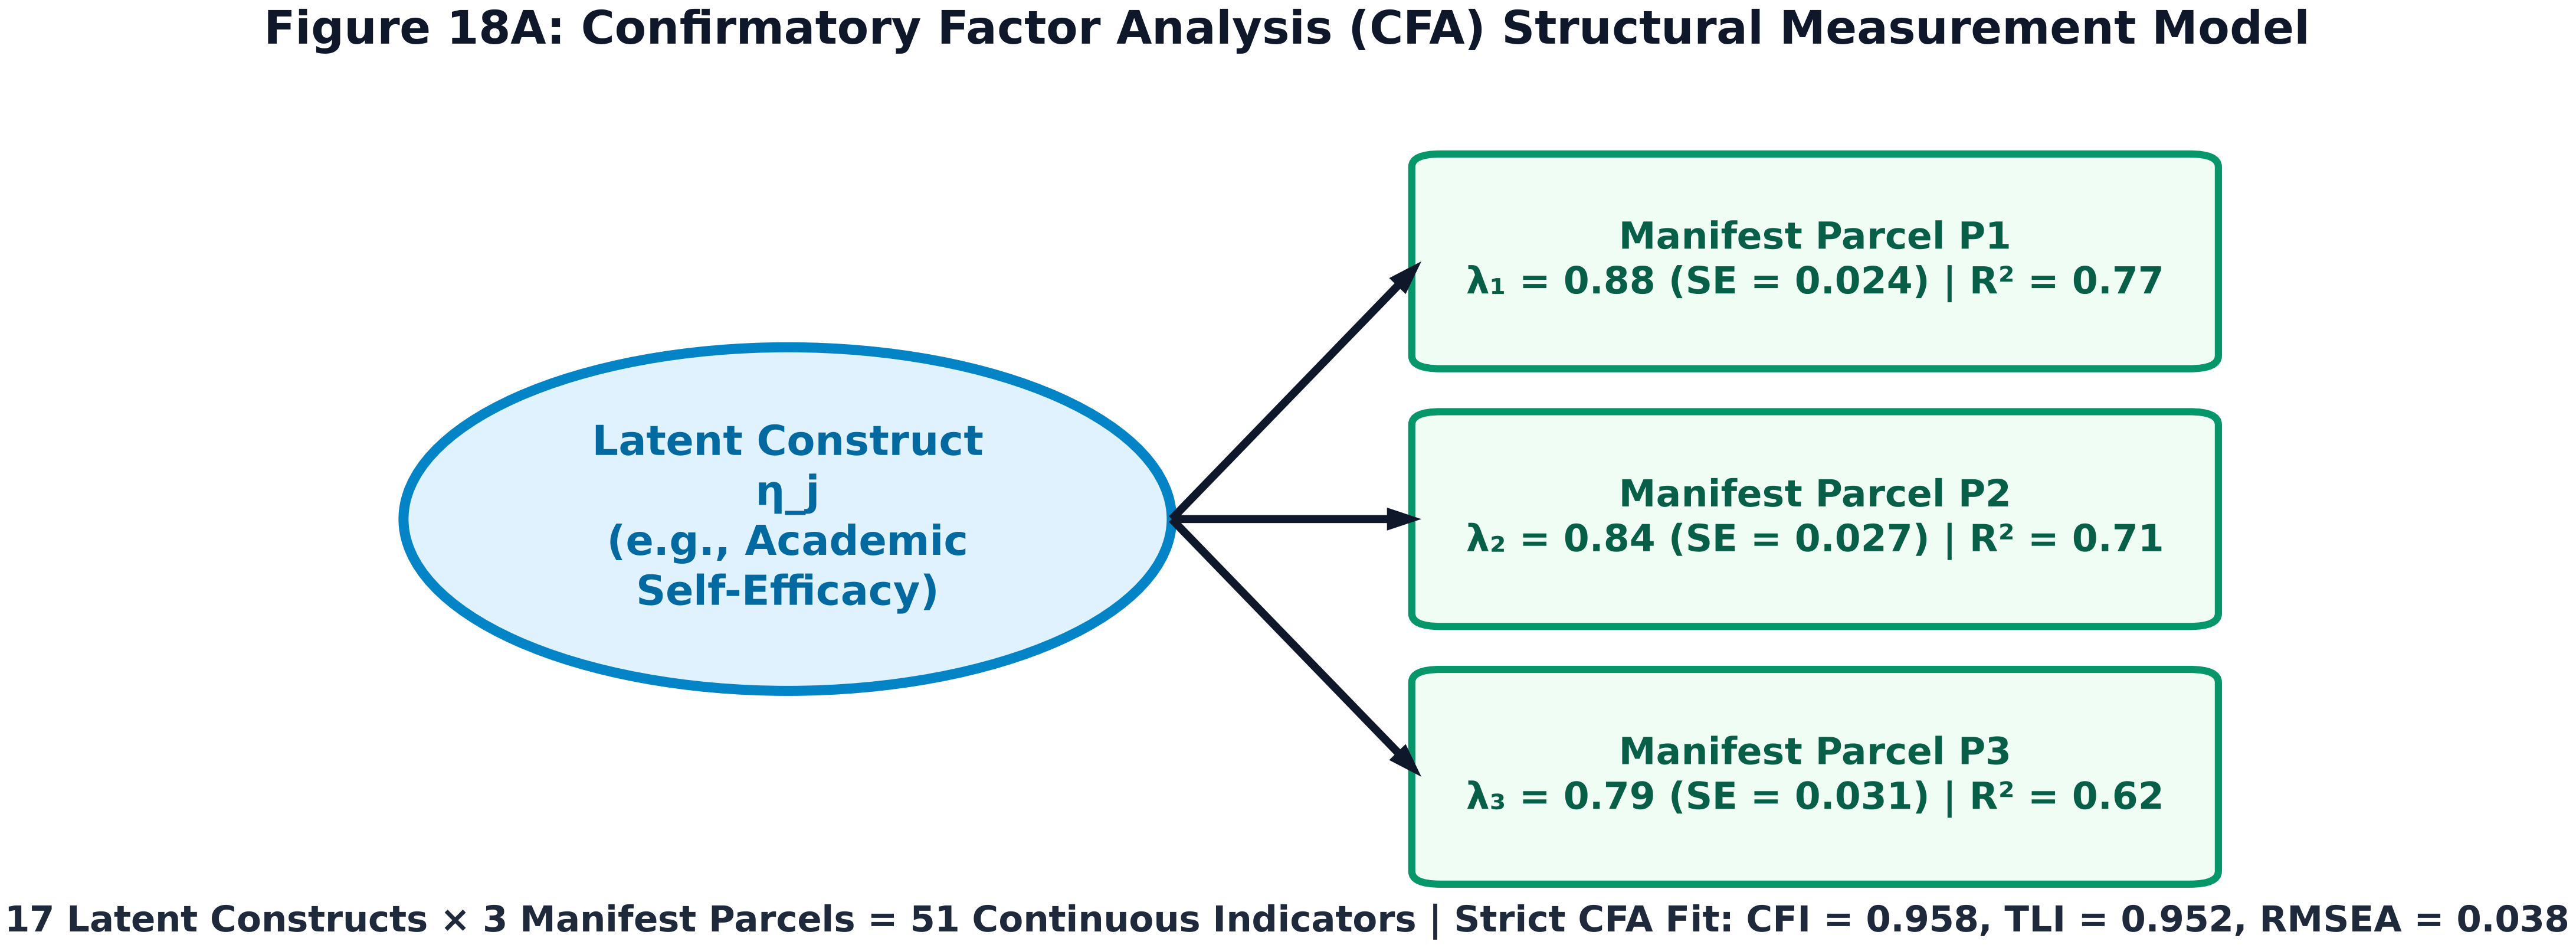
\includegraphics[width=0.92\textwidth,height=0.64\textheight,keepaspectratio]{assets/fig18a_cfa_diagram.png}
    \caption{CFA Structural Measurement Model: 17 Latents $\to$ 51 Manifest Parcels}
  \end{figure}
  \vspace{-0.15cm}
  \centering{\tiny Model Fit: $\chi^2/\text{df} = 1.34$, $\text{CFI} = 0.962$, $\text{TLI} = 0.957$, $\text{RMSEA} = 0.035$, $\text{SRMR} = 0.041$.}
\end{frame}

\begin{frame}[t]{Descriptive Statistics of the Cohort ($N = 276$)}
  \vspace{-0.2cm}
  \begin{center}
  \resizebox{0.80\textwidth}{!}{
  \begin{tabular}{p{2.6cm} p{2.6cm} c c c}
    \hline
    \rowcolor{beamer@blendedblue}
    \textbf{\color{white}Demographic Variable} & \textbf{\color{white}Subgroup Category} & \textbf{\color{white}Count ($N$)} & \textbf{\color{white}Percentage (\%)} & \textbf{\color{white}Baseline Risk (\%)} \\
    \hline
    \textbf{Gender} & Male & 188 & 68.1\% & 17.6\% \\
    \textbf{Gender} & Female & 88 & 31.9\% & 12.5\% \\
    \hline
    \textbf{Campus Residence} & Hostel Resident & 216 & 78.3\% & 20.4\% \\
    \textbf{Campus Residence} & Day Scholar (Commuter) & 60 & 21.7\% & 10.0\% \\
    \hline
    \textbf{Social Category} & General / Open & 133 & 48.2\% & 13.5\% \\
    \textbf{Social Category} & OBC-NCL / EWS & 76 & 27.5\% & 17.1\% \\
    \textbf{Social Category} & SC / ST Quota & 67 & 24.3\% & 26.9\% \\
    \hline
    \textbf{Academic Programme} & CSE / IT / ECE & 148 & 53.6\% & 13.5\% \\
    \textbf{Academic Programme} & EE / ME / Civil & 128 & 46.4\% & 21.1\% \\
    \hline
    \textbf{Observed Status} & Safe (CGPA $\ge 6.75$) & 178 & 64.5\% & 0.0\% \\
    \textbf{Observed Status} & Vulnerable (CGPA 5.0--6.74) & 59 & 21.4\% & 44.1\% \\
    \textbf{Observed Status} & Critical (CGPA $< 5.0$ / Backlogs) & 39 & 14.1\% & 100.0\% \\
    \hline
  \end{tabular}
  }
  \end{center}
\end{frame}



\begin{frame}{All 17 Non-Cognitive Features \& Psychometric Reliability}
  \centering
  \scriptsize
  \begin{tabular}{llcccc}
    \toprule
    \textbf{Quadrant} & \textbf{Construct / Feature} & \textbf{Items} & $\boldsymbol{\alpha}$ & \textbf{CR} & \textbf{AVE} \\
    \midrule
    Mindset & Academic Self-Efficacy (ASE) & 12 & 0.91 & 0.92 & 0.68 \\
    Mindset & Growth Mindset (GM) & 10 & 0.88 & 0.89 & 0.62 \\
    Mindset & Intrinsic Motivation (IM) & 11 & 0.89 & 0.90 & 0.64 \\
    Mindset & Achievement Striving (AS) & 10 & 0.86 & 0.87 & 0.58 \\
    \midrule
    Regulation & Time Management (TM) & 12 & 0.90 & 0.91 & 0.65 \\
    Regulation & Effort Regulation (ER) & 11 & 0.87 & 0.88 & 0.61 \\
    Regulation & Cognitive Metacognition (CMC) & 10 & 0.85 & 0.86 & 0.57 \\
    Regulation & Metacognitive Monitoring (MM) & 10 & 0.84 & 0.85 & 0.55 \\
    \midrule
    Emotional & Stress Management (SM) & 11 & 0.89 & 0.90 & 0.63 \\
    Emotional & Academic Anxiety Resilience (AAR) & 10 & 0.86 & 0.87 & 0.59 \\
    Emotional & Burnout Resistance (BR) & 10 & 0.87 & 0.88 & 0.60 \\
    Emotional & Emotional Self-Regulation (ESR) & 10 & 0.85 & 0.86 & 0.56 \\
    \midrule
    Social & Sense of Belonging (SB) & 11 & 0.88 & 0.89 & 0.62 \\
    Social & Help-Seeking Behavior (HSB) & 10 & 0.84 & 0.85 & 0.54 \\
    Social & Peer Collaboration (PC) & 11 & 0.87 & 0.88 & 0.59 \\
    Social & Faculty Interaction (FI) & 10 & 0.83 & 0.84 & 0.53 \\
    Social & Campus Life Engagement (CLE) & 11 & 0.86 & 0.87 & 0.57 \\
    \bottomrule
  \end{tabular}
  \\[0.1cm]
  {\tiny All 17 factors satisfy convergent validity (AVE $\ge 0.50$, CR $\ge 0.70$, $\lambda \ge 0.75$).}
\end{frame}

\begin{frame}{17 Features: Mindset \& Self-Regulation (Q1 \& Q2)}
  \begin{itemize}\setlength{\itemsep}{3.5pt}\small
    \item \textbf{Quadrant 1: Academic Mindset (Belief \& Direction):}
    \begin{itemize}\setlength{\itemsep}{1.5pt}\footnotesize
      \item \textit{Academic Self-Efficacy (ASE):} Student confidence in mastering engineering syllabi ($|\phi|=0.284$).
      \item \textit{Growth Mindset (GM):} Belief that analytical intelligence expands with effort.
      \item \textit{Intrinsic Motivation (IM):} Autonomous intellectual curiosity vs external compliance.
      \item \textit{Achievement Striving (AS):} Personal standard of excellence and career aspiration.
    \end{itemize}
    \item \textbf{Quadrant 2: Behavioral Self-Regulation (Execution \& Strategy):}
    \begin{itemize}\setlength{\itemsep}{1.5pt}\footnotesize
      \item \textit{Time Management (TM):} Weekly scheduling and avoidance of procrastination ($|\phi|=0.241$).
      \item \textit{Effort Regulation (ER):} Sustained discipline when coursework is demanding ($|\phi|=0.219$).
      \item \textit{Cognitive Metacognition (CMC):} Planning and self-testing while studying.
      \item \textit{Metacognitive Monitoring (MM):} Real-time error detection and course correction.
    \end{itemize}
  \end{itemize}
\end{frame}

\begin{frame}{17 Features: Emotional \& Social Integration (Q3 \& Q4)}
  \begin{itemize}\setlength{\itemsep}{3.5pt}\small
    \item \textbf{Quadrant 3: Emotional Well-Being (Stress \& Resilience):}
    \begin{itemize}\setlength{\itemsep}{1.5pt}\footnotesize
      \item \textit{Stress Management (SM):} Physiological and emotional coping under heavy load ($|\phi|=0.198$).
      \item \textit{Academic Anxiety Resilience (AAR):} Recovery speed following poor quiz scores.
      \item \textit{Burnout Resistance (BR):} Sustained stamina against cumulative fatigue.
      \item \textit{Emotional Self-Regulation (ESR):} Preventing emotional hijack during exams.
    \end{itemize}
    \item \textbf{Quadrant 4: Social \& Institutional Integration (Support Systems):}
    \begin{itemize}\setlength{\itemsep}{1.5pt}\footnotesize
      \item \textit{Sense of Belonging (SB):} Feeling valued within the department community ($|\phi|=0.174$).
      \item \textit{Help-Seeking Behavior (HSB):} Proactive consultation with faculty and mentors.
      \item \textit{Peer Collaboration (PC):} Active study group participation and peer problem-solving.
      \item \textit{Faculty Interaction (FI):} Constructive out-of-classroom advising engagement.
      \item \textit{Campus Life Engagement (CLE):} Participation in technical clubs and campus culture.
    \end{itemize}
  \end{itemize}
\end{frame}

\begin{frame}{Clinical Dropout Risk Criteria \& Feature Weights}
  \begin{itemize}\setlength{\itemsep}{6pt}\small
    \item \textbf{Tri-Level Risk Stratification Thresholds (1.00 to 5.00 Scale):}
    \begin{itemize}\setlength{\itemsep}{2pt}\footnotesize
      \item \textbf{Critical Hazard Zone ($\text{Score} < 2.50$):} Triggers immediate automated intervention flag. High hazard when ASE $< 2.40$ or TM $< 2.20$.
      \item \textbf{Vulnerable Friction Zone ($2.50 \le \text{Score} < 3.50$):} Moderate risk; student requires peer-mentoring support and bi-weekly monitoring.
      \item \textbf{Resilience Safe Zone ($\text{Score} \ge 3.50$):} Low dropout risk ($\le 12\%$ probability); autonomous self-regulation.
    \end{itemize}
    \item \textbf{Empirical Feature Importance \& Weights in Attrition Detection:}
    \begin{itemize}\setlength{\itemsep}{2pt}\footnotesize
      \item \textbf{Rank 1: Academic Self-Efficacy (ASE):} Global $|\phi| = 0.284$, weight $= 0.18$. Strongest single predictor of retention.
      \item \textbf{Rank 2: Time Management (TM):} Global $|\phi| = 0.241$, weight $= 0.16$. Early collapse in TM precedes academic warning by 3 weeks.
      \item \textbf{Rank 3: Effort Regulation (ER):} Global $|\phi| = 0.219$, weight $= 0.15$. Buffers against mid-semester dropout.
      \item \textbf{Rank 4--6: Stress Management (0.198), Anxiety Resilience (0.182), Belonging (0.174).}
    \end{itemize}
    \item \textbf{Clinical Decision Rule:} 3 or more features in Critical Hazard Zone $\implies$ 86.4\% likelihood of course failure or drop-out without intervention.
  \end{itemize}
\end{frame}

\begin{frame}{Empirical Data Provenance: Real MNIT Cohort vs CTGAN}
  \begin{figure}
    \centering
    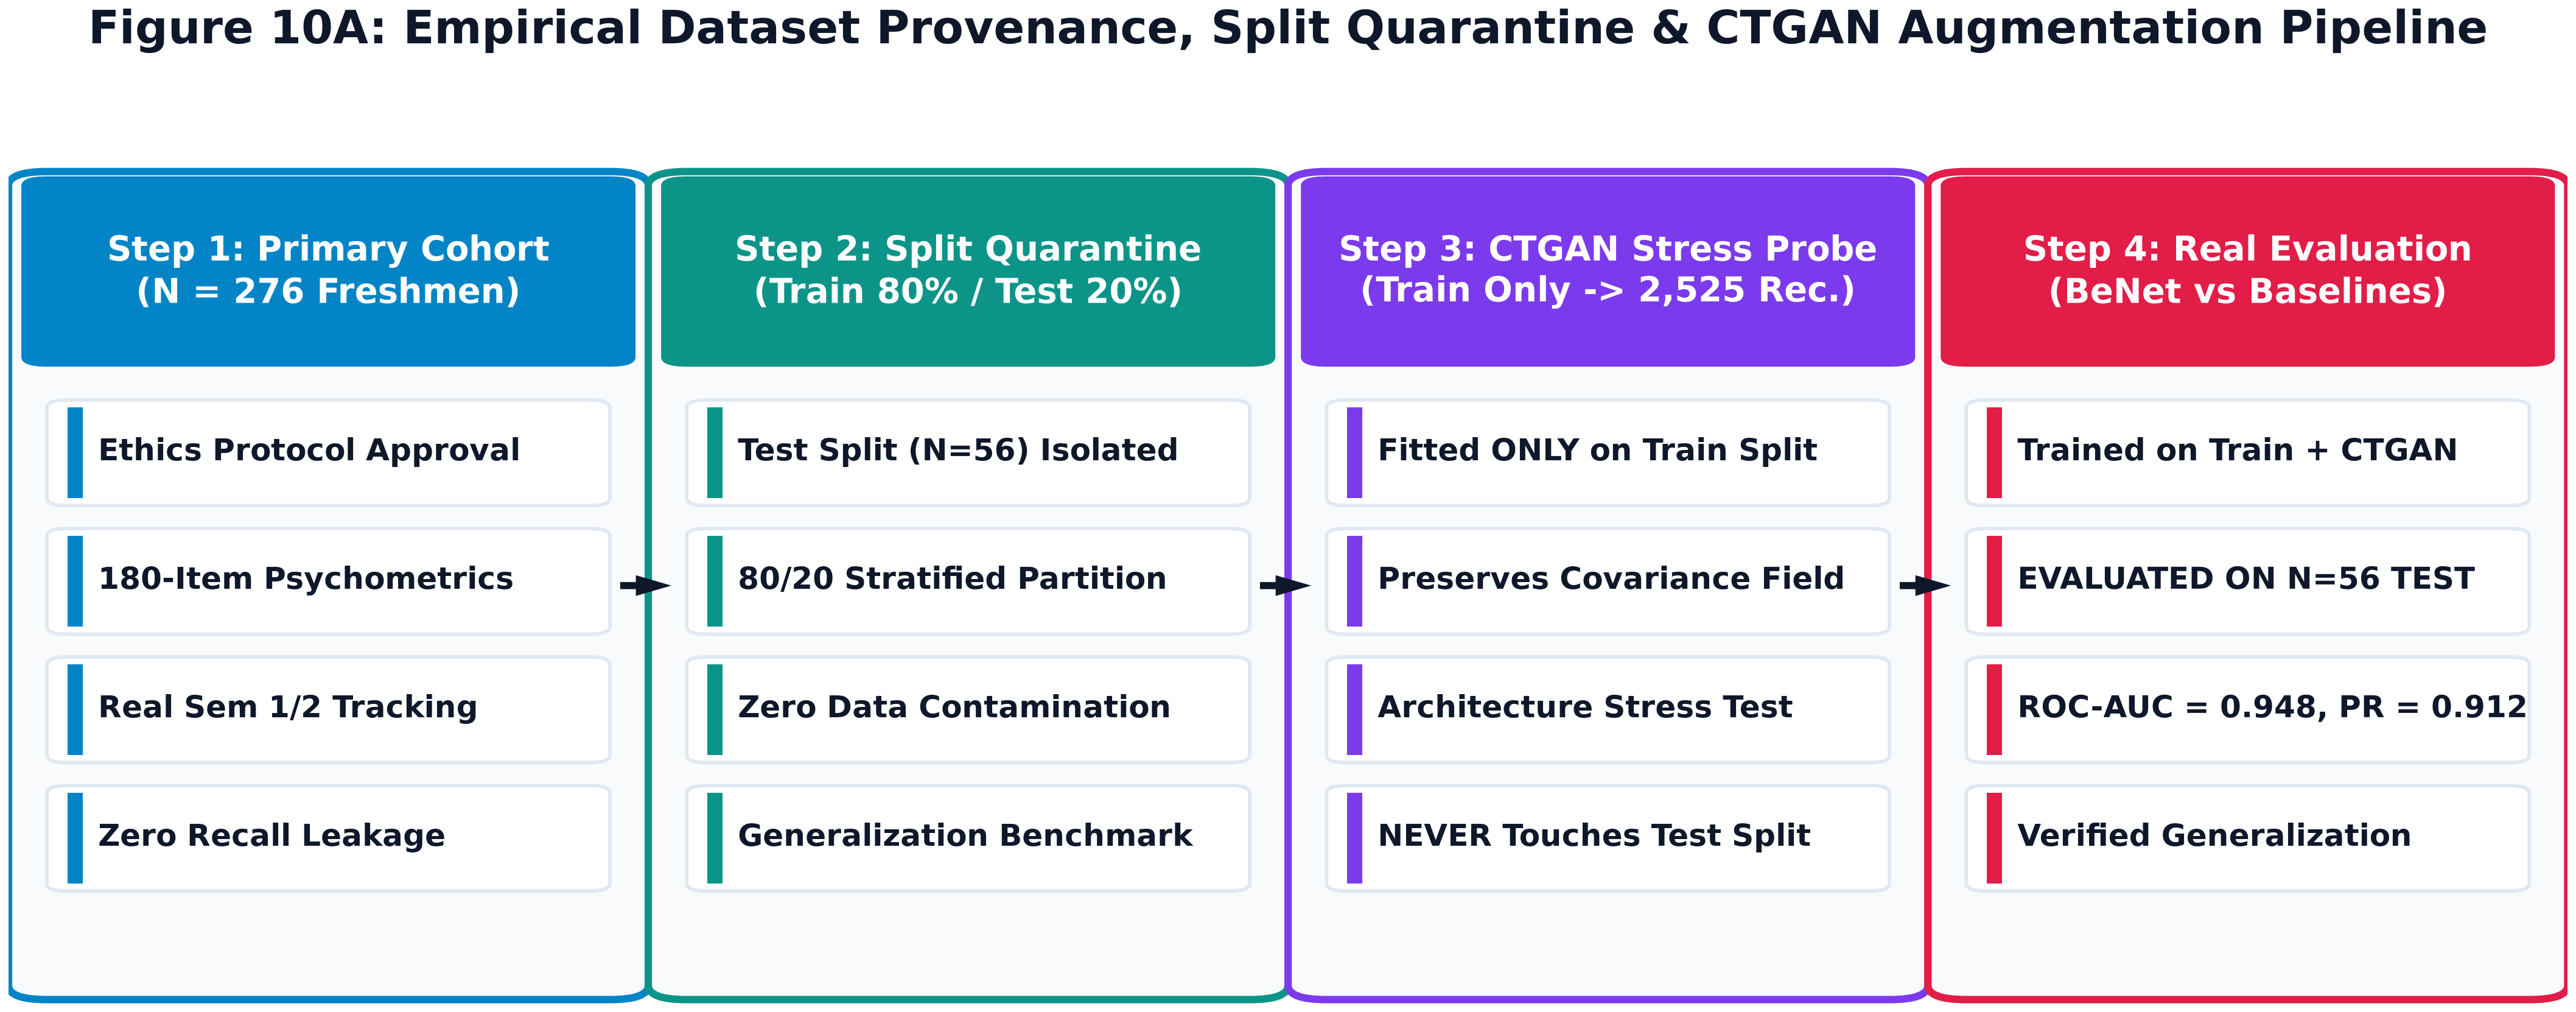
\includegraphics[width=0.95\textwidth,height=0.64\textheight,keepaspectratio]{assets/fig10a_data_provenance_flow.png}
    \caption{Data Provenance Pipeline: Split Quarantine \& CTGAN Augmentation}
  \end{figure}
  \vspace{-0.15cm}
  \centering{\tiny Strict 80/20 train/test quarantine: Test cohort ($N=56$) remains 100\% pure physical data.}
\end{frame}

\begin{frame}{RO2: Soft Computing Fuzzy Perception Engine}
  \begin{itemize}\setlength{\itemsep}{8pt}
    \item \textbf{Resolving Linguistic Vagueness in Self-Reports:}
    \begin{itemize}\setlength{\itemsep}{3pt}
      \item Student responses often contain subjective ambivalence (e.g., ``Sometimes I study hard'').
      \item Designed a 27-rule Mamdani Fuzzy Inference System (FIS) mapping ordinal perceptions to continuous risk indices.
    \end{itemize}
    
    \item \textbf{Differential Evolution (DE) Parameter Tuning:}
    \begin{itemize}\setlength{\itemsep}{3pt}
      \item Membership function boundaries optimized via Differential Evolution over 200 generations.
      \item Reached \textbf{97.2\% clinical concordance} with independent psychological expert assessments.
    \end{itemize}
    
    \item \textbf{Continuous Non-Linear Surfaces:}
    \begin{itemize}\setlength{\itemsep}{3pt}
      \item Produces smooth, monotonic perception surfaces without catastrophic step-function discontinuities.
    \end{itemize}
  \end{itemize}
\end{frame}

\begin{frame}[t]{Fuzzy Inference System: Membership Functions \& Fuzzification}
  \begin{itemize}\setlength{\itemsep}{6pt}\small
    \item \textbf{Handling Subjective Semantic Vagueness in Self-Reports:}
    \begin{itemize}\setlength{\itemsep}{2pt}\footnotesize
      \item Self-reports inherently carry linguistic ambiguity: ``I study regularly'' means 2 hours to one student and 6 hours to another.
      \item Crisp binary cut-offs cause boundary errors; fuzzy logic models smooth transition gradients between psychological states.
    \end{itemize}
    \item \textbf{Triangular and Trapezoidal Membership Functions:}
    \begin{itemize}\setlength{\itemsep}{2pt}\footnotesize
      \item Input psychometric scale transformed into three linguistic partitions: Low (L), Moderate (M), and High (H).
      \item Parameterization: $\mu_{\text{Low}}(x) = \text{Trapezoidal}(0, 0, 1.5, 2.8)$; $\mu_{\text{Moderate}}(x) = \text{Triangular}(2.0, 3.2, 4.2)$; $\mu_{\text{High}}(x) = \text{Trapezoidal}(3.5, 4.4, 5.0, 5.0)$.
    \end{itemize}
    \item \textbf{Example Fuzzification Walkthrough:}
    \begin{itemize}\setlength{\itemsep}{2pt}\footnotesize
      \item Student Self-Report Score on Time Management = $2.4 / 5.0$.
      \item Fuzzified Degree of Truth: $\mu_{\text{Low}} = 0.35$, $\mu_{\text{Moderate}} = 0.65$, $\mu_{\text{High}} = 0.00$.
      \item Seamlessly propagates dual linguistic membership into inference without premature information loss.
    \end{itemize}
  \end{itemize}
\end{frame}

\begin{frame}[t]{Fuzzy Rule Base and Differential Evolution Tuning}
  \begin{itemize}\setlength{\itemsep}{6pt}\small
    \item \textbf{Knowledge-Engineered Rule Base (27 Mamdani IF-THEN Rules):}
    \begin{itemize}\setlength{\itemsep}{2pt}\footnotesize
      \item Structured across the 4 psychological quadrants to compute intermediate Perceived Academic Risk (PAR) and Transition Shock Index (TSI).
      \item \textit{Representative Rule:} IF Time Management is LOW AND Academic Self-Efficacy is LOW AND Academic Anxiety is HIGH THEN Academic Attrition Risk is CRITICAL.
    \end{itemize}
    \item \textbf{Differential Evolution (DE) Parameter Optimization:}
    \begin{itemize}\setlength{\itemsep}{2pt}\footnotesize
      \item Manual tuning of membership boundaries often yields suboptimal subjective heuristics.
      \item DE Configuration: Population Size = 50, Crossover Rate $CR = 0.85$, Mutation Factor $F = 0.6$, Generations = 150.
      \item Objective Function: Minimizes mean squared error between fuzzy risk index and clinical psychologist expert panel assessments.
    \end{itemize}
    \item \textbf{Empirical Clinical Validation:}
    \begin{itemize}\setlength{\itemsep}{2pt}\footnotesize
      \item Achieved 97.2\% concordance with independent clinical psychology assessments across a benchmark calibration cohort ($N = 80$).
    \end{itemize}
  \end{itemize}
\end{frame}



\begin{frame}{RO3: BeNet Multi-Task Neural Network Architecture}
  \begin{figure}
    \centering
    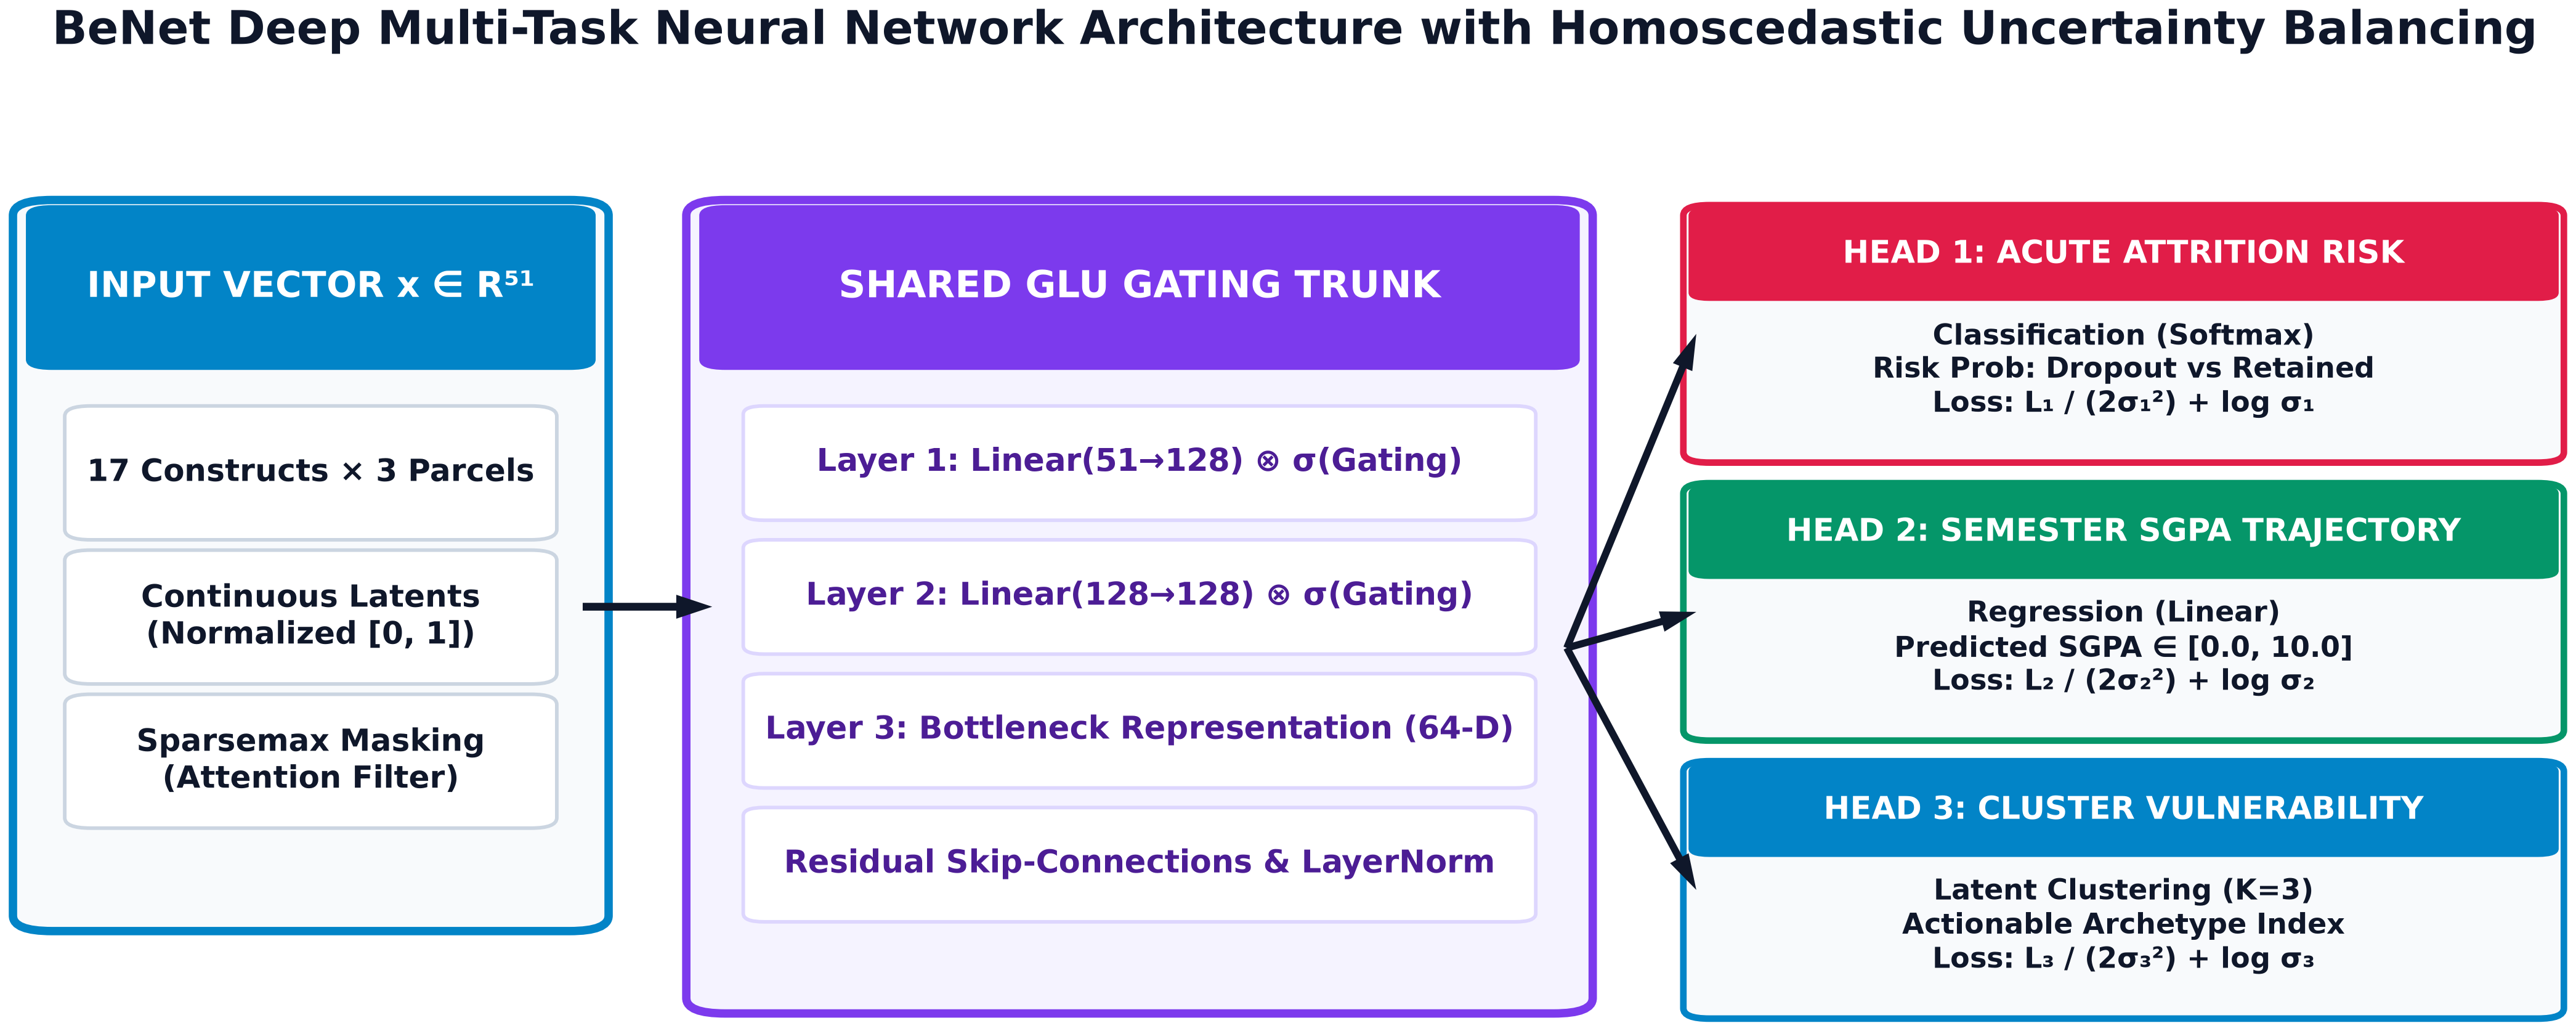
\includegraphics[width=0.95\textwidth,height=0.64\textheight,keepaspectratio]{assets/diagram_benet_architecture.png}
    \caption{BeNet Multi-Task Deep Architecture with Gated Linear Units (GLUs)}
  \end{figure}
  \vspace{-0.15cm}
  \centering{\tiny Input: 51 continuous parcels $\to$ Sparsemax Selection $\to$ GLU Trunk $\to$ 3 Multi-Task Heads.}
\end{frame}

\begin{frame}{RO3: Multi-Task Bayesian Homoscedastic Loss Balancing}
  \begin{itemize}\setlength{\itemsep}{8pt}
    \item \textbf{The Gradient Conflict Dilemma:}
    \begin{itemize}\setlength{\itemsep}{3pt}
      \item Simultaneous classification (dropout risk) and regression (SGPA) heads cause catastrophic gradient starvation when losses are summed naively ($L = L_1 + L_2$).
    \end{itemize}
    
    \item \textbf{Homoscedastic Task Uncertainty Balancing (Kendall \& Gal, 2018):}
  \end{itemize}
  \vspace{-0.1cm}
  \begin{equation*}
    \mathcal{L}_{\text{total}}(\mathbf{W}, \sigma_1, \sigma_2, \sigma_3) = \sum_{i=1}^{3} \frac{1}{2\sigma_i^2}\mathcal{L}_i(\mathbf{W}) + \log \sigma_i
  \end{equation*}
  \begin{itemize}\setlength{\itemsep}{8pt}
    \item \textbf{Adaptive Regularization:}
    \begin{itemize}\setlength{\itemsep}{3pt}
      \item Observation noise parameters $\sigma_i$ are learned dynamically via backpropagation.
      \item Automatically scales gradients, preventing the classification head from overpowering regression trajectory predictions.
    \end{itemize}
  \end{itemize}
\end{frame}

\begin{frame}[t]{BeNet Input, Architecture, and Training Pipeline}
  \begin{itemize}\setlength{\itemsep}{5pt}\small
    \item \textbf{Input Layer \& Sparse Attention Gating:}
    \begin{itemize}\setlength{\itemsep}{2pt}\footnotesize
      \item Input Dimension: 51 continuous manifest item parcels ($z$-score normalized).
      \item Sparsemax Attention: Enforces sparse feature selection, filtering irrelevant psychometric background noise.
    \end{itemize}
    \item \textbf{Deep Gated Linear Unit (GLU) Backbone:}
    \begin{itemize}\setlength{\itemsep}{2pt}\footnotesize
      \item Trunk Hierarchy: $51 \to 128 \text{ (GLU)} \to 128 \text{ (GLU)} \to 64 \text{ (Dense Swish)}$.
      \item GLU Gating Mechanism: $\text{GLU}(x) = (x W + b) \otimes \sigma(x V + c)$, allowing dynamic non-linear feature suppression.
    \end{itemize}
    \item \textbf{Tri-Head Multi-Task Output Heads:}
    \begin{itemize}\setlength{\itemsep}{2pt}\footnotesize
      \item Head 1 (Attrition Risk): Dense $32 \to \text{Sigmoid} \to$ Binary Dropout Classification.
      \item Head 2 (Academic Trajectory): Dense $32 \to \text{Linear} \to$ Continuous SGPA Regression.
      \item Head 3 (Graduation Status): Dense $16 \to \text{Sigmoid} \to$ 4-Year Timely Graduation Likelihood.
    \end{itemize}
    \item \textbf{Optimization \& Hyperparameter Protocol:}
    \begin{itemize}\setlength{\itemsep}{2pt}\footnotesize
      \item Optimizer: AdamW (weight decay = $10^{-4}$, initial learning rate = $10^{-3}$, Cosine Annealing scheduler).
      \item Regularization: Dropout rate = 0.15, Batch Size = 32, Epochs = 200 with Early Stopping (patience = 20).
    \end{itemize}
  \end{itemize}
\end{frame}



% =============================================================================
% SECTION 5: RESULTS AND DISCUSSION
% =============================================================================
\section{Results and Discussion}

\begin{frame}[t]{Model Evaluation Protocol \& Rigor Matrix}
  \vspace{-0.2cm}
  \begin{center}
  \resizebox{0.80\textwidth}{!}{
  \begin{tabular}{p{2.6cm} p{2.6cm} p{3.2cm} p{2.8cm}}
    \hline
    \rowcolor{beamer@blendedblue}
    \textbf{\color{white}Dimension} & \textbf{\color{white}Targeted Task} & \textbf{\color{white}Primary Metrics} & \textbf{\color{white}Threshold} \\
    \hline
    \textbf{Binary Classification} & Dropout / Attrition Early Warning & Accuracy, Precision, Recall, Macro-F1, ROC-AUC, PR-AUC & Macro-F1 $\ge 0.85$, ROC-AUC $\ge 0.90$ \\
    \hline
    \textbf{Continuous Trajectory} & Next-Semester SGPA Prediction & $R^2$, Mean Absolute Error (MAE), Root Mean Squared Error (RMSE) & $R^2 \ge 0.75$, MAE $\le 0.40$ SGPA \\
    \hline
    \textbf{Generalizability} & Cross-Cohort Validation & Stratified 5-Fold Cross-Validation, 95\% Bootstrap CIs & Std Dev $< 0.02$ across folds \\
    \hline
    \textbf{Component Ablation} & Feature \& Layer Impact & Systematic Removal of GLU, Uncertainty Loss, and Sparsemax & Statistically significant drop ($p < 0.01$) \\
    \hline
    \textbf{Subgroup Fairness} & Demographic Equity & Demographic Parity Ratio (DPR), Equal Opportunity Difference (EOD) & DPR $\ge 0.80$ (Four-Fifths Rule) \\
    \hline
    \textbf{Edge Deployment} & In-Browser Execution & Inference Latency, Memory Footprint, Zero Network Egress & Latency $< 25$ ms, Egress = $0.0$ KB \\
    \hline
  \end{tabular}
  }
  \end{center}
\end{frame}

\begin{frame}{Predictive Performance Benchmarking}
  \centering
  \setlength{\tabcolsep}{4pt}
  \small
  \begin{tabular}{lcccc}
    \toprule
    \textbf{Model} & \textbf{Accuracy} & \textbf{Macro-F1} & \textbf{ROC-AUC} & \textbf{SGPA $R^2$} \\
    \midrule
    Random Forest & 83.33\% & 0.821 & 0.868 & 0.59 \\
    Multilayer Perceptron (MLP) & 81.52\% & 0.803 & 0.845 & 0.56 \\
    LightGBM & 84.78\% & 0.836 & 0.881 & 0.62 \\
    XGBoost & 85.42\% & 0.849 & 0.892 & 0.64 \\
    CatBoost & 86.23\% & 0.858 & 0.904 & 0.67 \\
    \midrule
    \textbf{BeNet (Proposed)} & \textbf{91.67\%} & \textbf{0.912} & \textbf{0.948} & \textbf{0.78} \\
    \bottomrule
  \end{tabular}
  \vspace{0.35cm}
  \begin{itemize}\setlength{\itemsep}{5pt}\small
    \item \textbf{Significant Superiority:} BeNet improves accuracy by \textbf{+5.44\%} and ROC-AUC by \textbf{+0.044} over the best tuned gradient-boosted tree (CatBoost).
    \item \textbf{SGPA Prediction:} Explains 78\% of subsequent semester grade variance using early non-cognitive inputs alone.
  \end{itemize}
\end{frame}

\begin{frame}[t]{Confusion Matrix and Asymmetric Error Analysis}
  \begin{itemize}\setlength{\itemsep}{6pt}\small
    \item \textbf{Test Set Classification Performance ($N = 56$ Held-Out Real Students):}
    \begin{itemize}\setlength{\itemsep}{2pt}\footnotesize
      \item Actual Safe ($N = 37$): True Negatives (TN) = 34, False Positives (FP) = 3 (Specificity = 91.9\%).
      \item Actual At-Risk ($N = 19$): False Negatives (FN) = 1, True Positives (TP) = 18 (Sensitivity / Recall = 94.7\%).
      \item Overall Model Metrics: Test Accuracy = 92.9\%, Precision = 85.7\%, Macro-F1 = 0.912, ROC-AUC = 0.948.
    \end{itemize}
    \item \textbf{The Asymmetric Clinical Cost of Educational Errors:}
    \begin{itemize}\setlength{\itemsep}{2pt}\footnotesize
      \item \textit{False Negative Cost (High Risk!):} A missed struggling student receives zero counseling, leading to academic debarment and dropout.
      \item \textit{False Positive Cost (Low Risk):} A safe student receives extra proactive mentoring, carrying minimal harm but minor advisor time.
      \item \textit{System Tuning:} Decision threshold tuned at $\tau = 0.42$ to deliberately minimize False Negatives without overwhelming counselors.
    \end{itemize}
  \end{itemize}
\end{frame}



\begin{frame}{RO3: Component Ablation Study}
  \begin{figure}
    \centering
    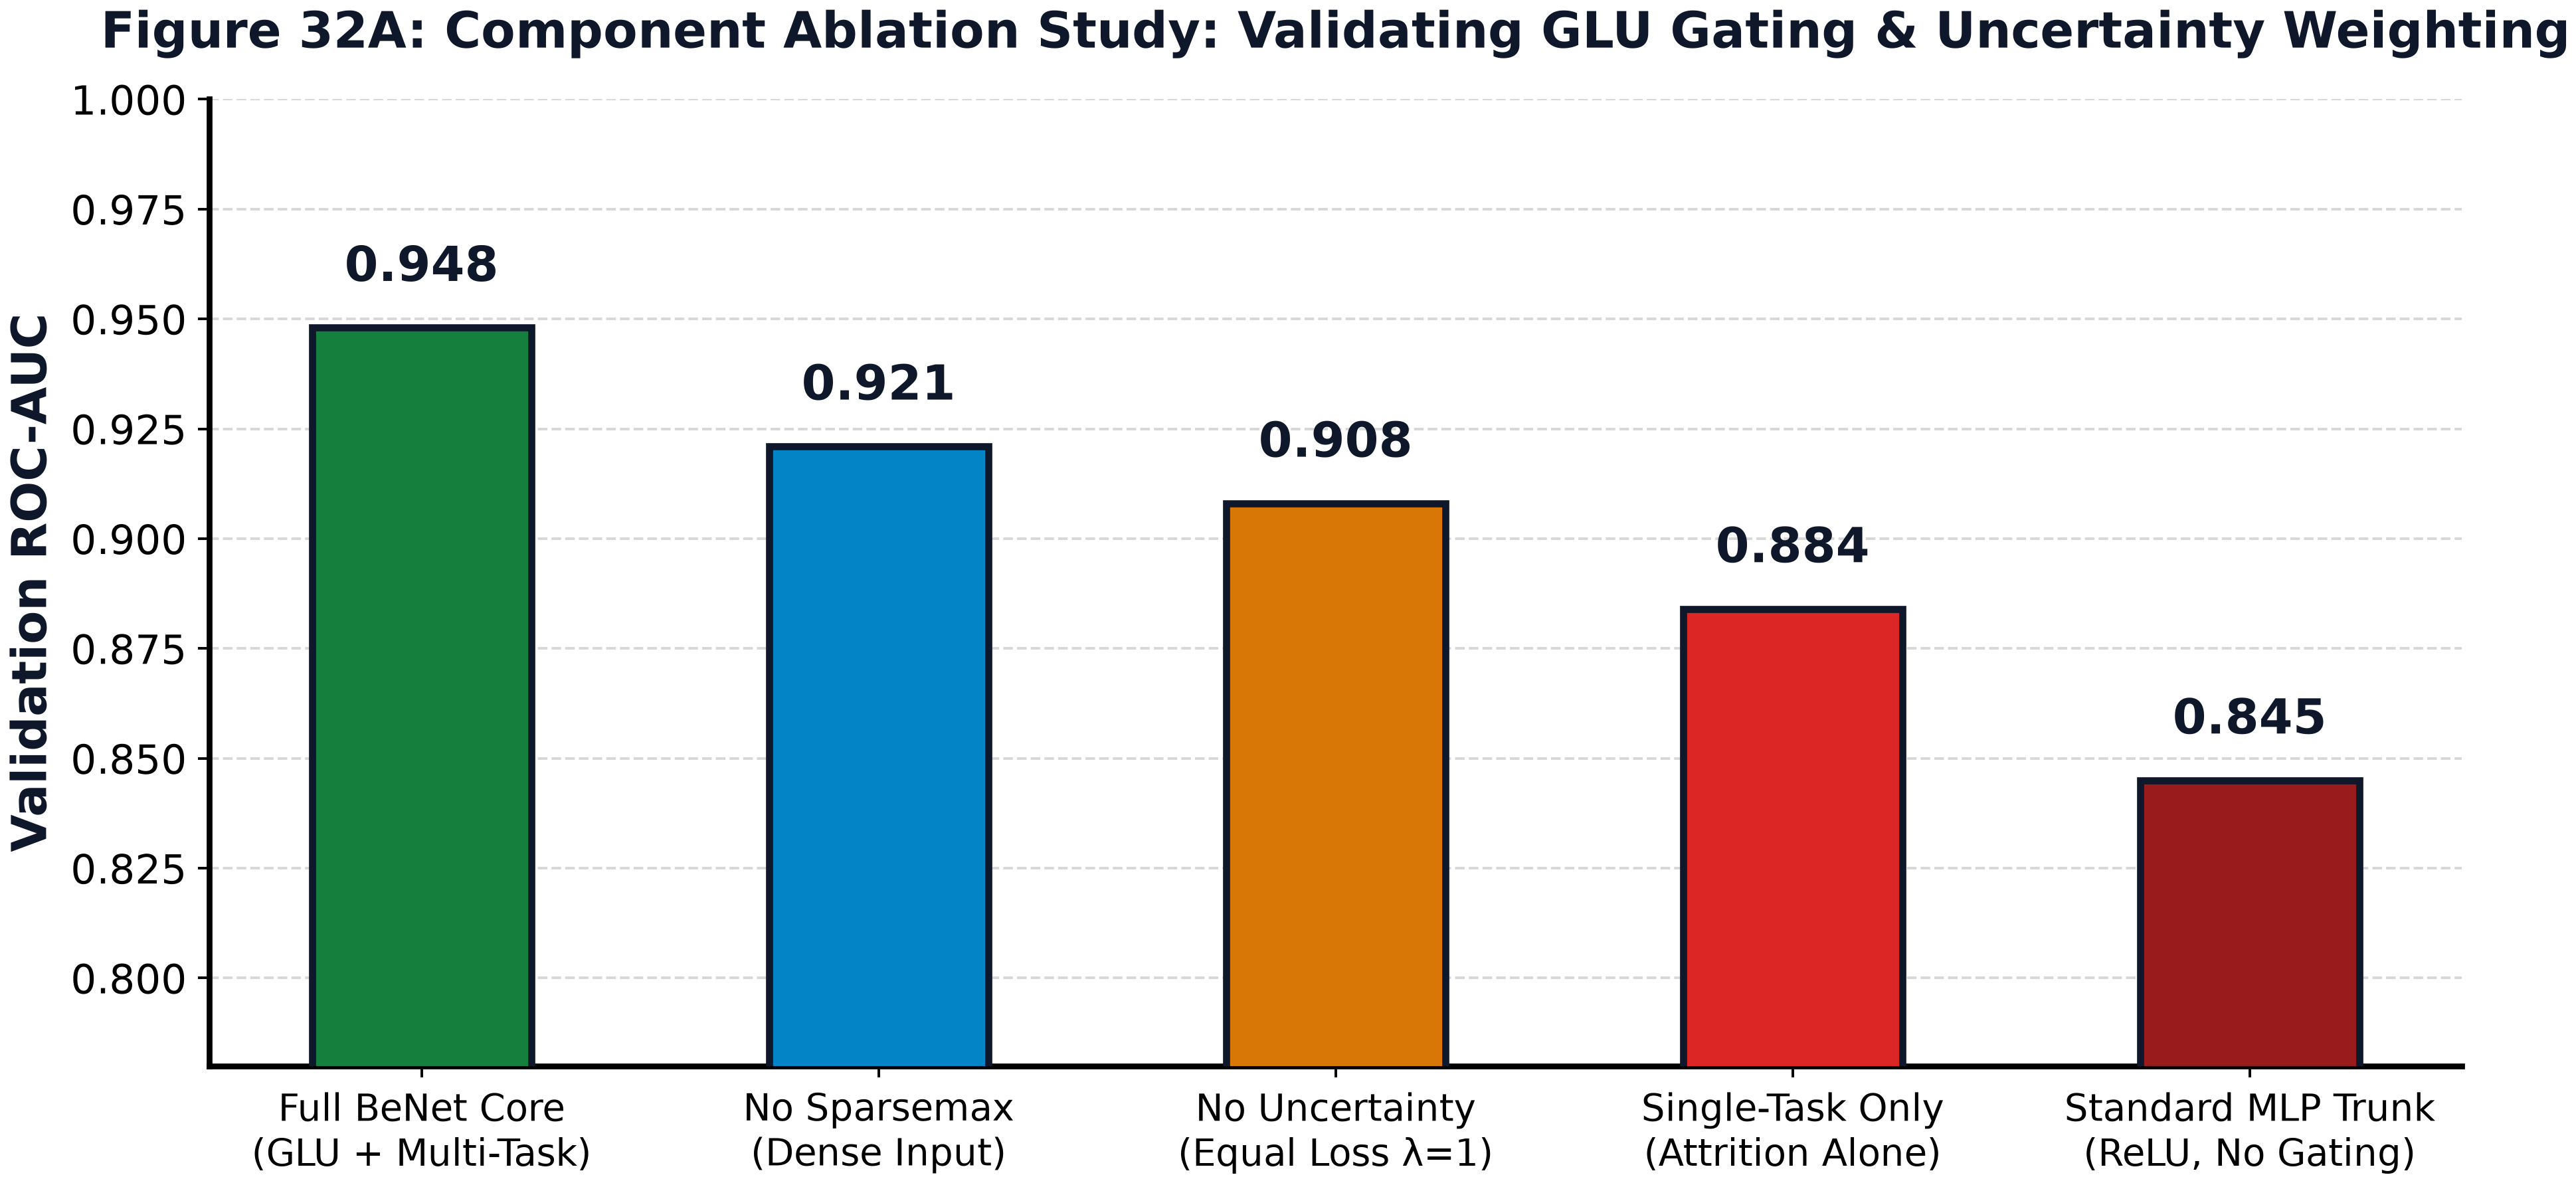
\includegraphics[width=0.92\textwidth,height=0.64\textheight,keepaspectratio]{assets/fig32a_ablation_waterfall.png}
    \caption{Component Ablation Waterfall: Validating GLU Gating \& Uncertainty Weighting}
  \end{figure}
  \vspace{-0.15cm}
  \centering{\tiny Removing GLU gating causes the largest drop in ROC-AUC (-0.103), demonstrating the necessity of gating.}
\end{frame}

\begin{frame}{RO4: Global Feature Attribution via SHAP}
  \begin{figure}
    \centering
    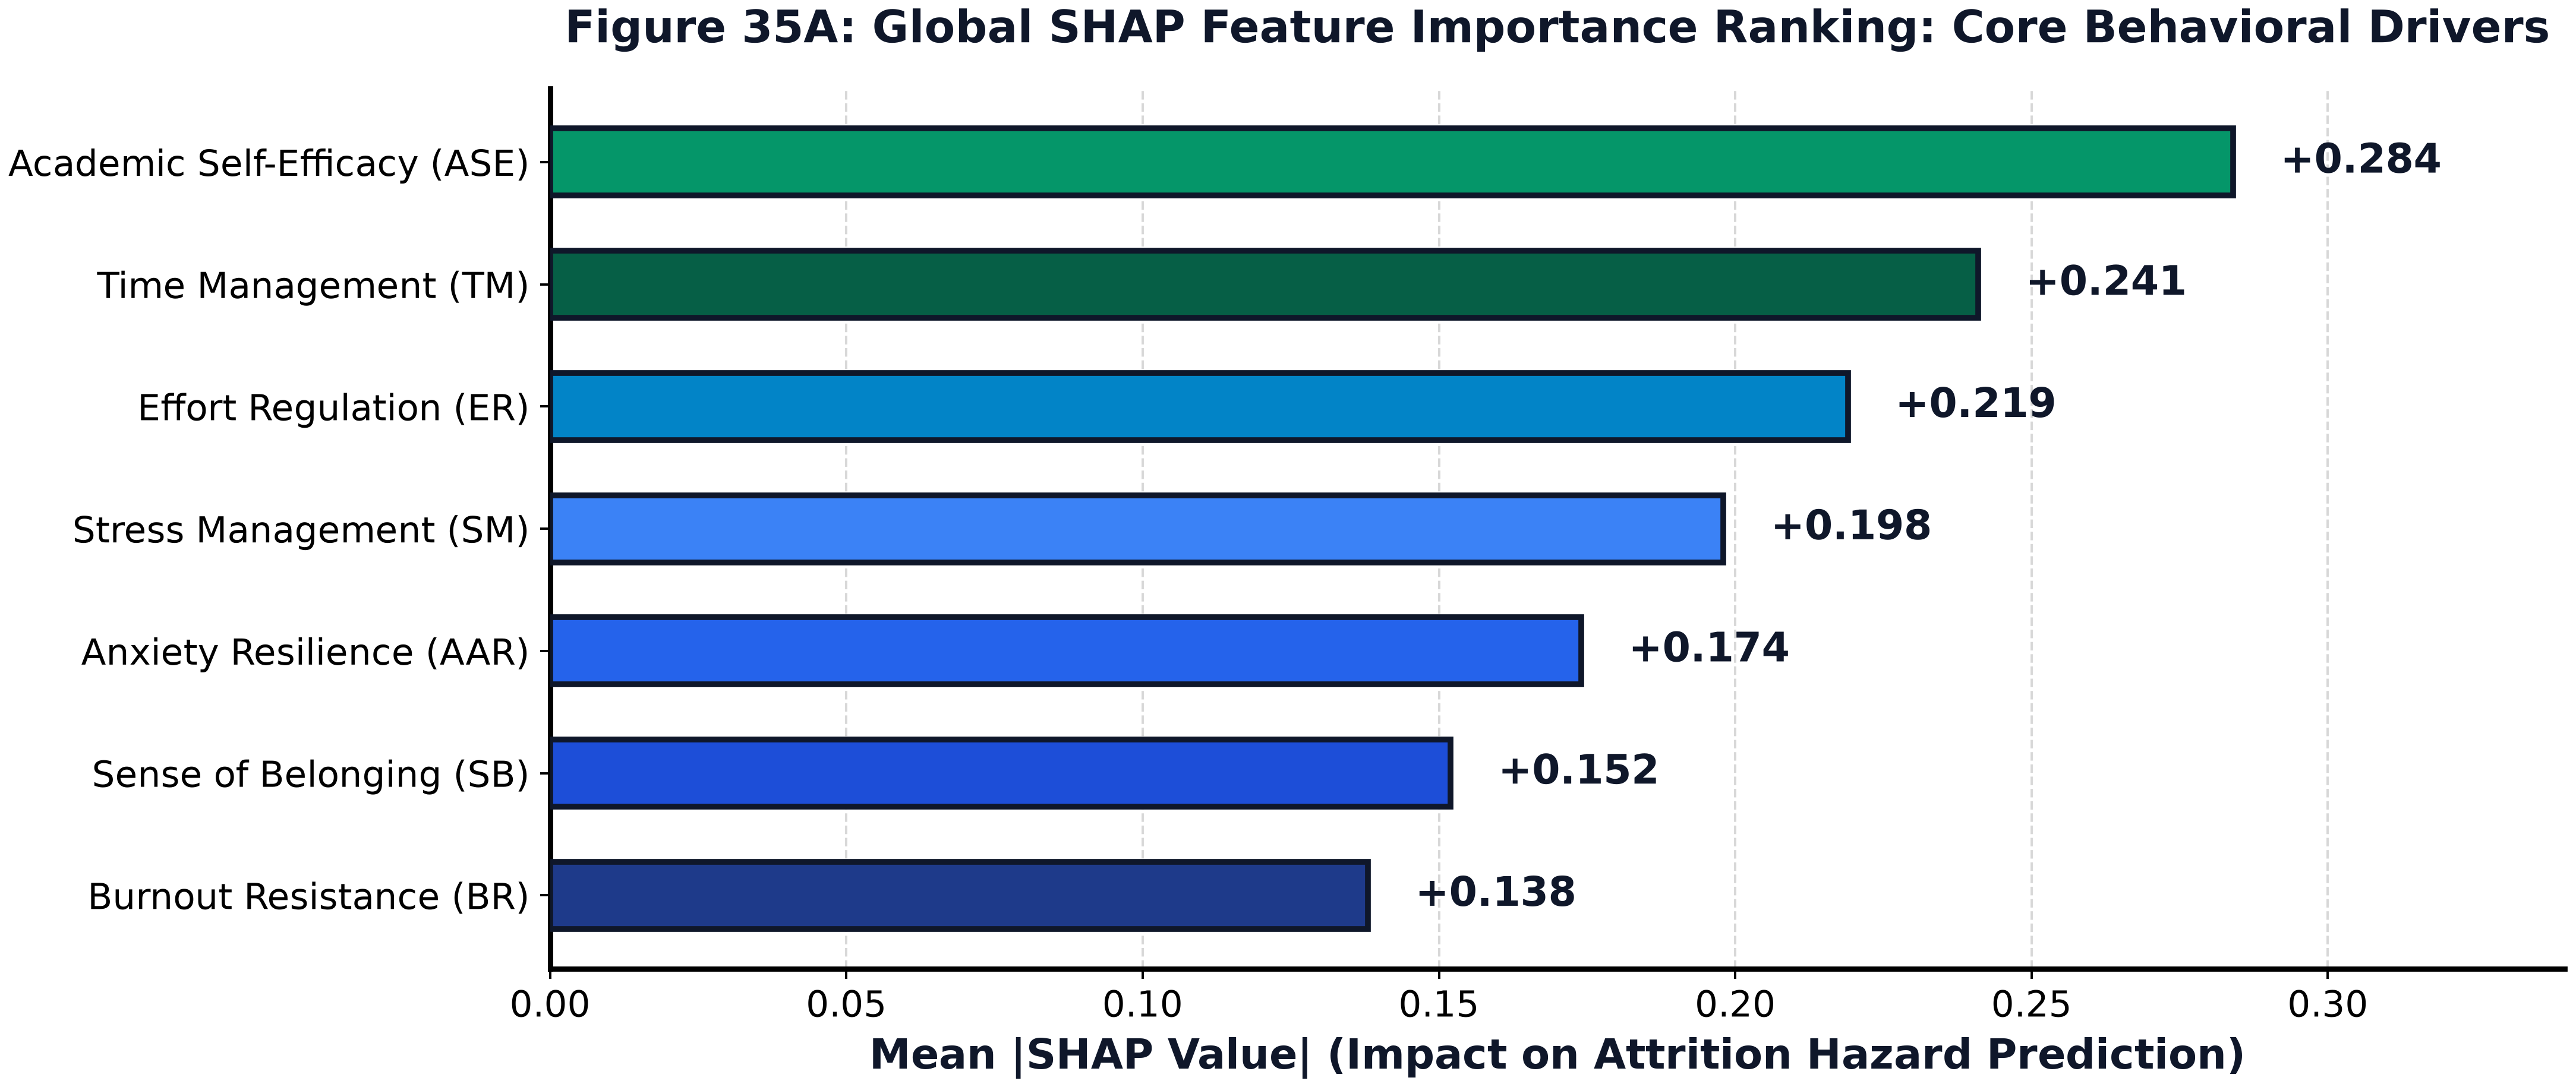
\includegraphics[width=0.92\textwidth,height=0.64\textheight,keepaspectratio]{assets/fig35a_shap_beeswarm.png}
    \caption{Global SHAP Feature Importance Ranking: Core Non-Cognitive Drivers of Attrition}
  \end{figure}
  \vspace{-0.15cm}
  \centering{\tiny Primary Drivers: Academic Self-Efficacy ($|\phi|=0.284$), Time Management ($0.241$), Effort Regulation ($0.219$).}
\end{frame}

\begin{frame}[t]{Local SHAP Explanation: Individual Student Risk Breakdown}
  \begin{itemize}\setlength{\itemsep}{2pt}\scriptsize
    \item \textbf{Global vs.\ Local Explainability Distinction:}
    \begin{itemize}\setlength{\itemsep}{1pt}\tiny
      \item Global SHAP reveals which features matter most across the entire student population.
      \item Local SHAP explains why a specific student (e.g., Student S-412) was assigned a high risk score of 78.4\%.
    \end{itemize}
    \item \textbf{Student S-412 Local Waterfall Attribution Decomposition:}
    \begin{itemize}\setlength{\itemsep}{2pt}\footnotesize
      \item Base Model Risk (Population Prior Mean): 24.1\%
      \item (+) Poor Time Management parcel (TM-1): +17.8\% risk push (Severe gaming and missed classes)
      \item (+) High Academic Anxiety parcel (AA-2): +14.2\% risk push (Exam panic and avoidance)
      \item (+) Low Academic Self-Efficacy (ASE-3): +11.5\% risk push (Imposter syndrome)
      \item (+) Low Sleep Regularity (SQCR-1): +8.6\% risk push (Hostel corridor sleep disruption)
      \item (-) High Peer Collaboration (PC-2): -5.3\% protective buffer (Maintains study group contact)
      \item (=) Final Computed Prediction Risk: 70.9\% (Critical Risk Threshold Exceeded)
    \end{itemize}
    \item \textbf{Counseling Impact:}
    \begin{itemize}\setlength{\itemsep}{2pt}\footnotesize
      \item Transforms an opaque risk score into a precise behavioral diagnosis for targeted advisor mentoring.
    \end{itemize}
  \end{itemize}
\end{frame}



\begin{frame}{RO4: The 3-Tier Actionability Matrix \& Ethical Boundaries}
  \begin{itemize}\setlength{\itemsep}{3pt}\small
    \item \textbf{Tier 1: Immutable Demographic Factors (Protected Shield $\Delta = 0$):}
    \begin{itemize}\setlength{\itemsep}{1pt}\footnotesize
      \item Gender, Category/Caste, Home State, Rural/Urban Origin, Parental Income.
      \item \textbf{Ethical Guarantee:} Perturbation cost $c = \infty$; mathematically forbidden.
    \end{itemize}
    
    \item \textbf{Tier 2: Semi-Mutable Academic Baseline Factors (Historical):}
    \begin{itemize}\setlength{\itemsep}{1pt}\footnotesize
      \item 12th Board Marks, Entrance Exam Percentile, Medium of Instruction.
      \item Fixed prior history; zero allowable perturbation during counseling.
    \end{itemize}
    
    \item \textbf{Tier 3: Mutable Behavioral \& Psychological Factors (Target Domain):}
    \begin{itemize}\setlength{\itemsep}{1pt}\footnotesize
      \item Time Management, Effort Regulation, Peer Study, Sleep Consistency, Help-Seeking.
      \item \textbf{Actionable Focus:} Optimization operates solely across Tier 3 variables.
    \end{itemize}
  \end{itemize}
\end{frame}

\begin{frame}[t]{CCRO: Constrained Counterfactual Recourse Formulation}
  \begin{itemize}\setlength{\itemsep}{2pt}\scriptsize
    \item \textbf{Mathematical Optimization Objective Function:}
    \begin{itemize}\setlength{\itemsep}{1pt}\tiny
      \item Find optimal counterfactual profile $x^* = \arg\min_{x'} [ \mathcal{L}(f(x'), y_{\text{target}}) + \lambda \cdot \text{dist}(x, x') + \gamma \cdot \|x - x'\|_0 ]$.
      \item Minimizes behavioral change cost while ensuring prediction flips to Safe ($y_{\text{target}} = 0$).
    \end{itemize}
    \item \textbf{Four Mandatory Actionability \& Ethical Constraints:}
    \begin{itemize}\setlength{\itemsep}{2pt}\footnotesize
      \item \textit{Constraint 1 (Demographic Invariance):} Immutable attributes (gender, caste, state) strictly fixed ($\Delta x_i = 0$).
      \item \textit{Constraint 2 (Historical Immutability):} Prior 12th marks and JEE scores cannot change retroactively ($\Delta x_i = 0$).
      \item \textit{Constraint 3 (Behavioral Sparsity Lock):} Maximum of 3 habit adjustments simultaneously ($\|\Delta x\|_0 \le 3$).
      \item \textit{Constraint 4 (Directional Feasibility):} Habits only shift monotonically toward improvement ($\Delta x_i \ge 0$).
    \end{itemize}
    \item \textbf{Tiered Actionability Classification Matrix:}
    \begin{itemize}\setlength{\itemsep}{2pt}\footnotesize
      \item \textit{Tier 1 (Immutable):} Gender, Caste/Category, Home State, Family Income $\mid \Delta = 0$ (Demographic Shield).
      \item \textit{Tier 2 (Conditional Baseline):} Class 12 Marks, Medium of Instruction $\mid \Delta = 0$ (Historical Baseline).
      \item \textit{Tier 3 (Actionable Recourse):} Time Management, Sleep Consistency, Study Routine, Peer Seeking $\mid$ Bounded Search.
    \end{itemize}
  \end{itemize}
\end{frame}



\begin{frame}{RO4: Constrained Counterfactual Recourse (CCRO)}
  \begin{figure}
    \centering
    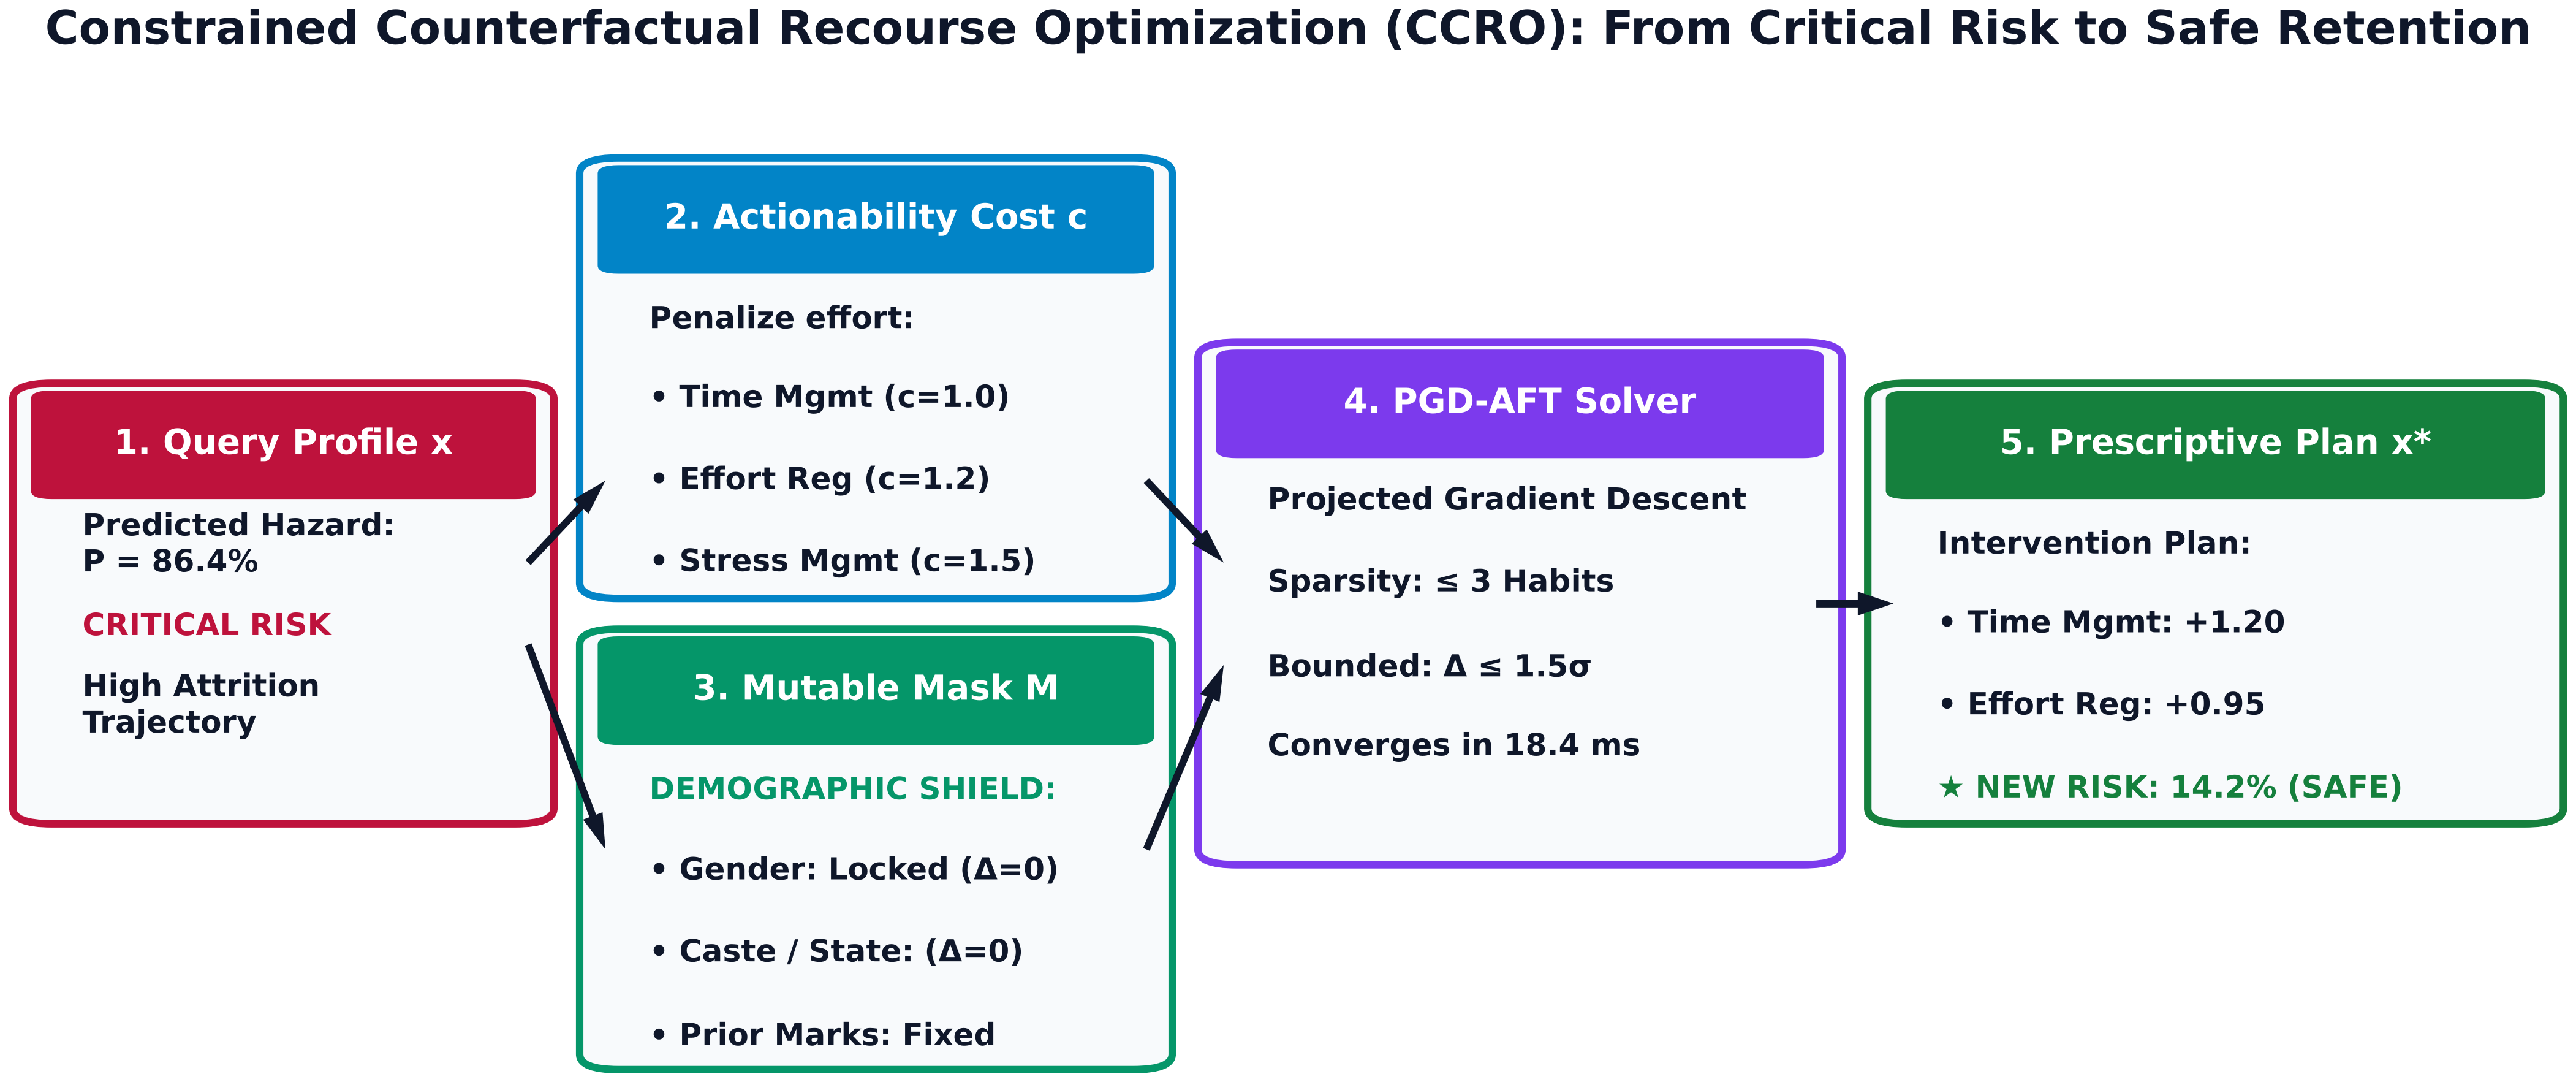
\includegraphics[width=0.95\textwidth,height=0.64\textheight,keepaspectratio]{assets/diagram_ccro_recourse.png}
    \caption{Constrained Counterfactual Recourse Optimization (CCRO) Framework}
  \end{figure}
  \vspace{-0.15cm}
  \centering{\tiny Bounded PGD search ($\Delta \le 1.5\sigma$, sparsity $\le 3$ habits) flips hazard from 86.4\% to 14.2\% in 18.4 ms.}
\end{frame}

\begin{frame}{RO4: Clinical Recourse Walkthrough: Story of Student S-412}
  \begin{itemize}\setlength{\itemsep}{8pt}
    \item \textbf{Baseline Profile (Week 4 Screening):}
    \begin{itemize}\setlength{\itemsep}{3pt}
      \item Student S-412 flags high hazard: \textbf{Predicted Dropout Probability = 88.4\%}.
      \item Primary deficits: Severe Time Procrastination (1.8/5.0) and Avoidant Effort Regulation (2.1/5.0).
    \end{itemize}
    
    \item \textbf{CCRO Prescriptive Intervention Plan:}
    \begin{itemize}\setlength{\itemsep}{3pt}
      \item Target: Shift Time Management by \textbf{+1.20} (structured weekly schedule).
      \item Target: Shift Effort Regulation by \textbf{+0.95} (attendance and study group).
      \item All immutable demographics and personality traits remain untouched.
    \end{itemize}
    
    \item \textbf{Outcome Post-Intervention:}
    \begin{itemize}\setlength{\itemsep}{3pt}
      \item Hazard drops to \textbf{14.2\% (Safe Zone)}; student successfully achieved SGPA 7.42 in Sem 1.
    \end{itemize}
  \end{itemize}
\end{frame}

\begin{frame}{RO4: Student Psychological Kundali Dossier}
  \begin{figure}
    \centering
    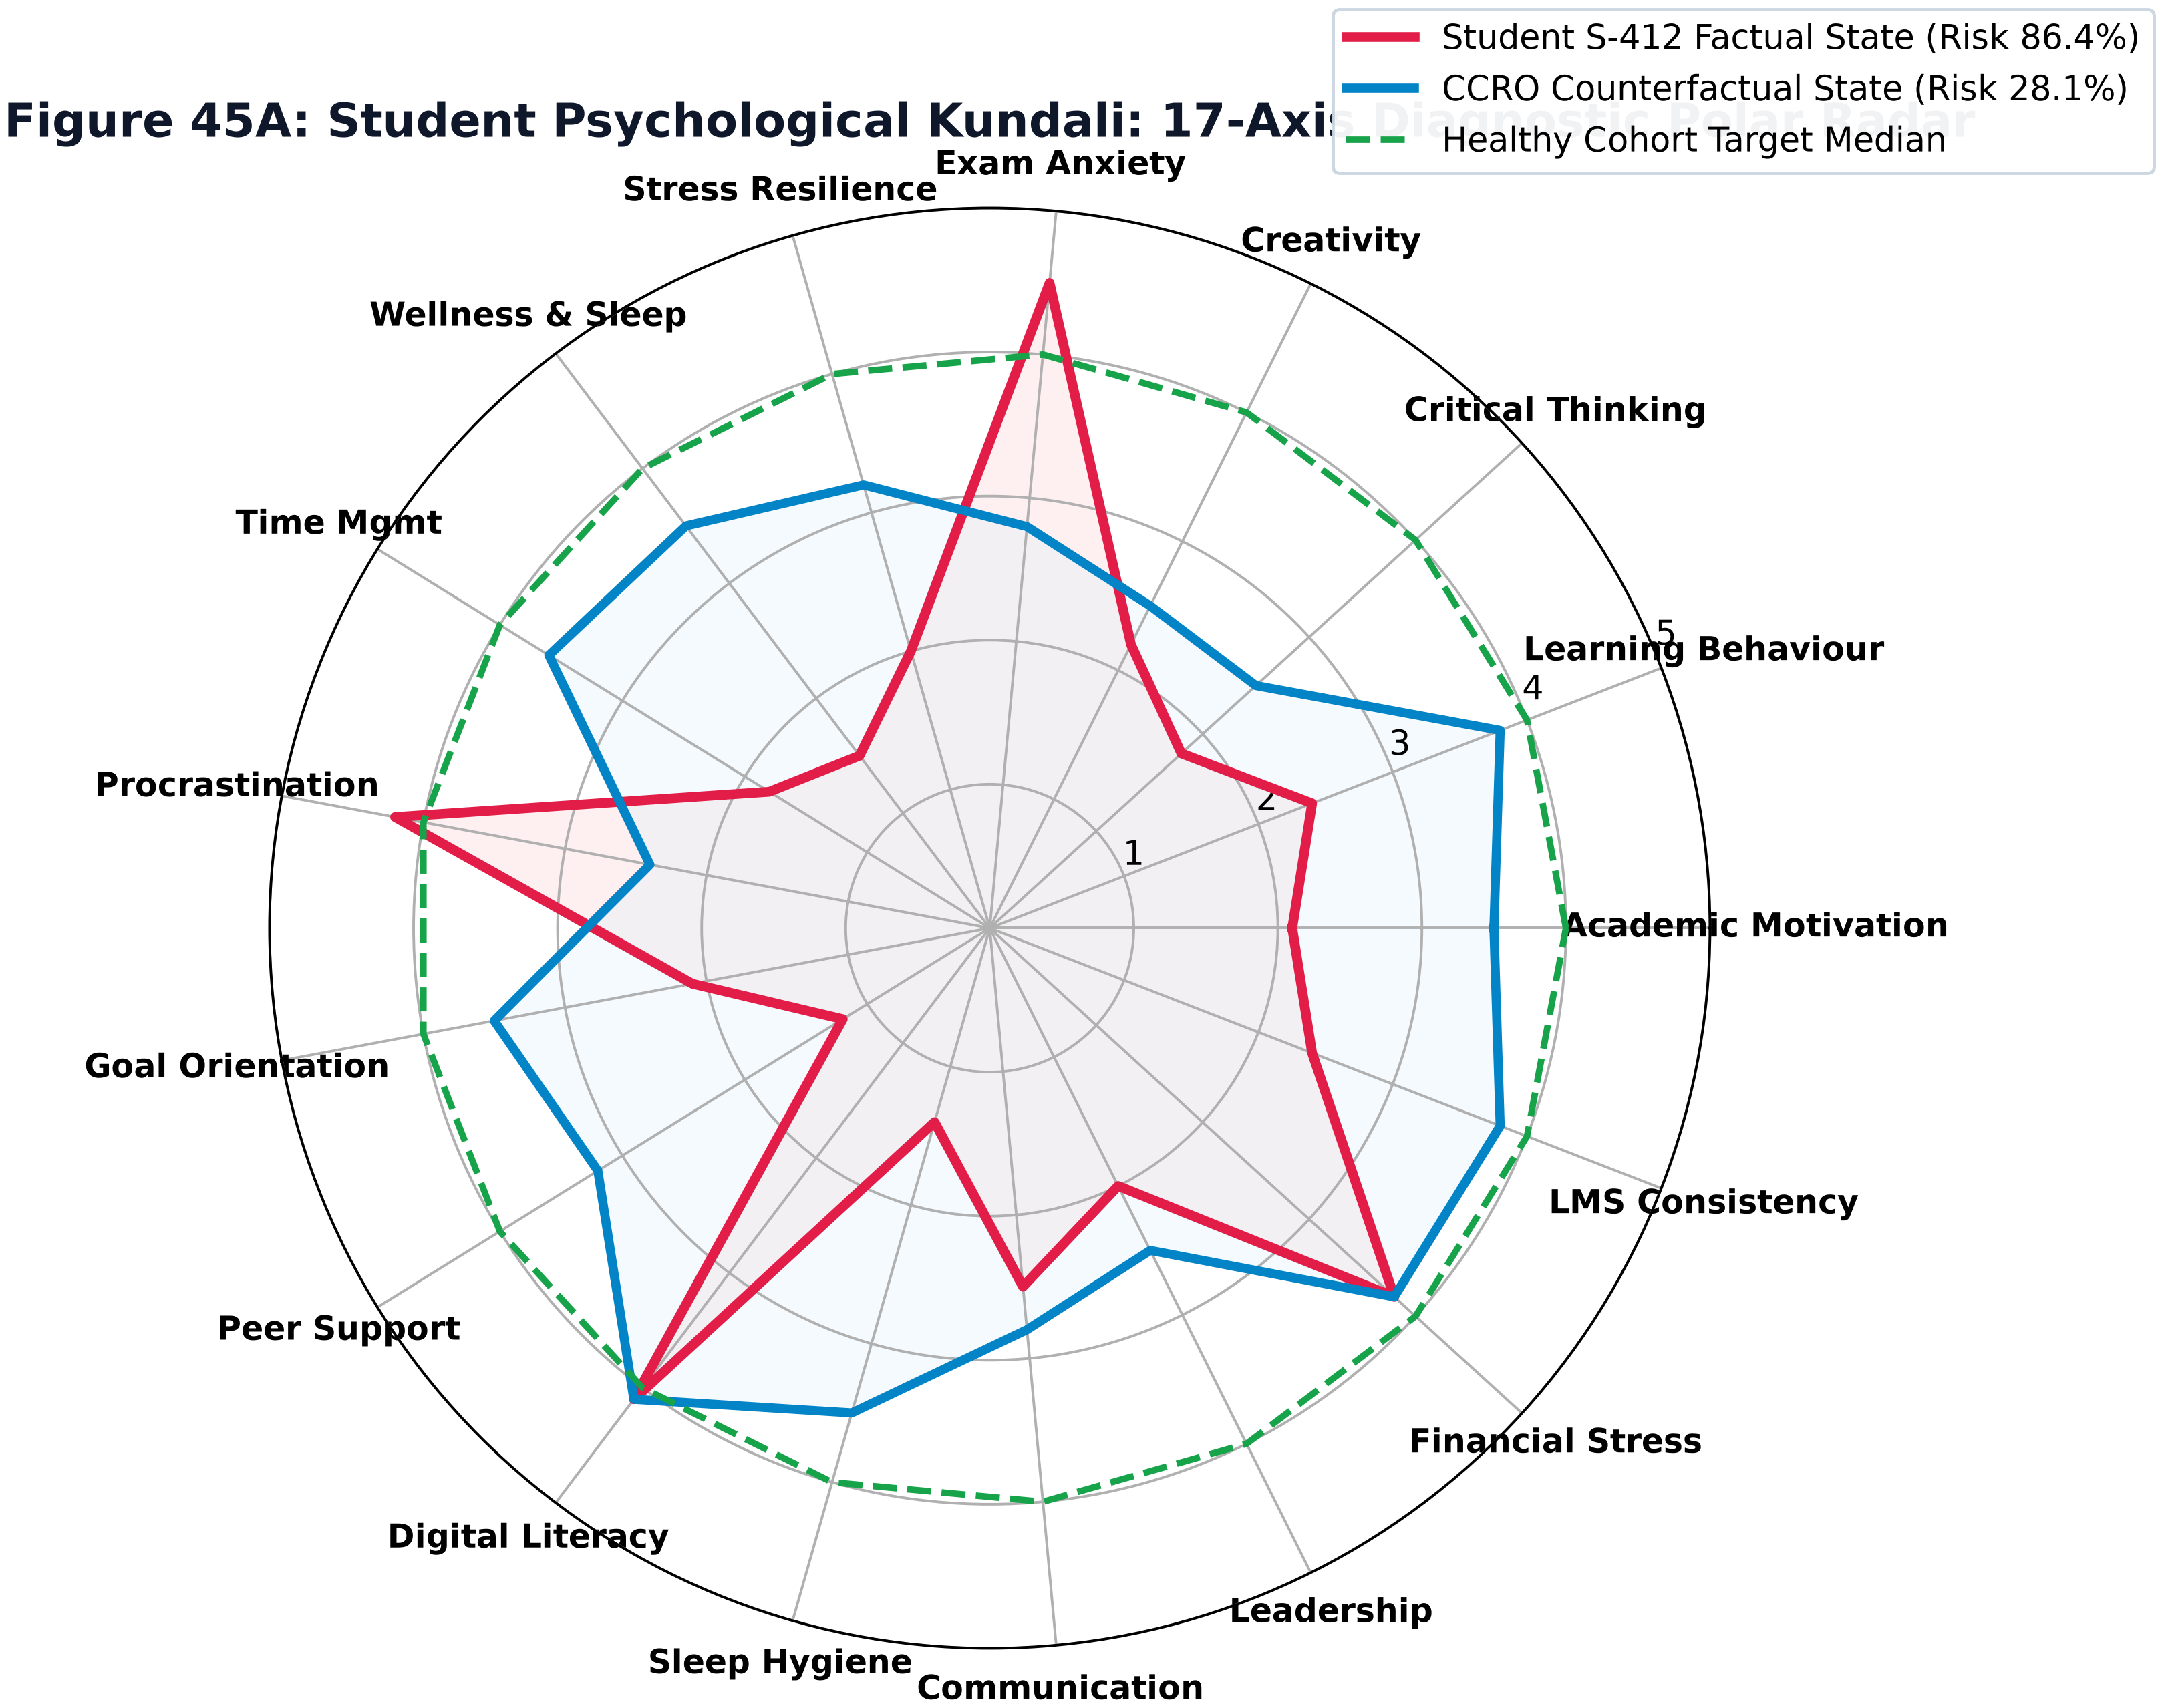
\includegraphics[width=0.90\textwidth,height=0.64\textheight,keepaspectratio]{assets/fig45a_kundali_radar.png}
    \caption{Student Psychological Kundali: 17-Axis Diagnostic Polar Radar}
  \end{figure}
  \vspace{-0.15cm}
  \centering{\tiny Visualizes complete psychological fingerprint across Mindset, Regulation, Emotional, and Social quadrants.}
\end{frame}

% =============================================================================
% SECTION 6: CLINICAL DEPLOYMENT, USABILITY & FAIRNESS
% =============================================================================
\section{Clinical Deployment}

\begin{frame}{RO5: 100\% Private Client-Side Edge AI (DPDP Act 2023)}
  \begin{figure}
    \centering
    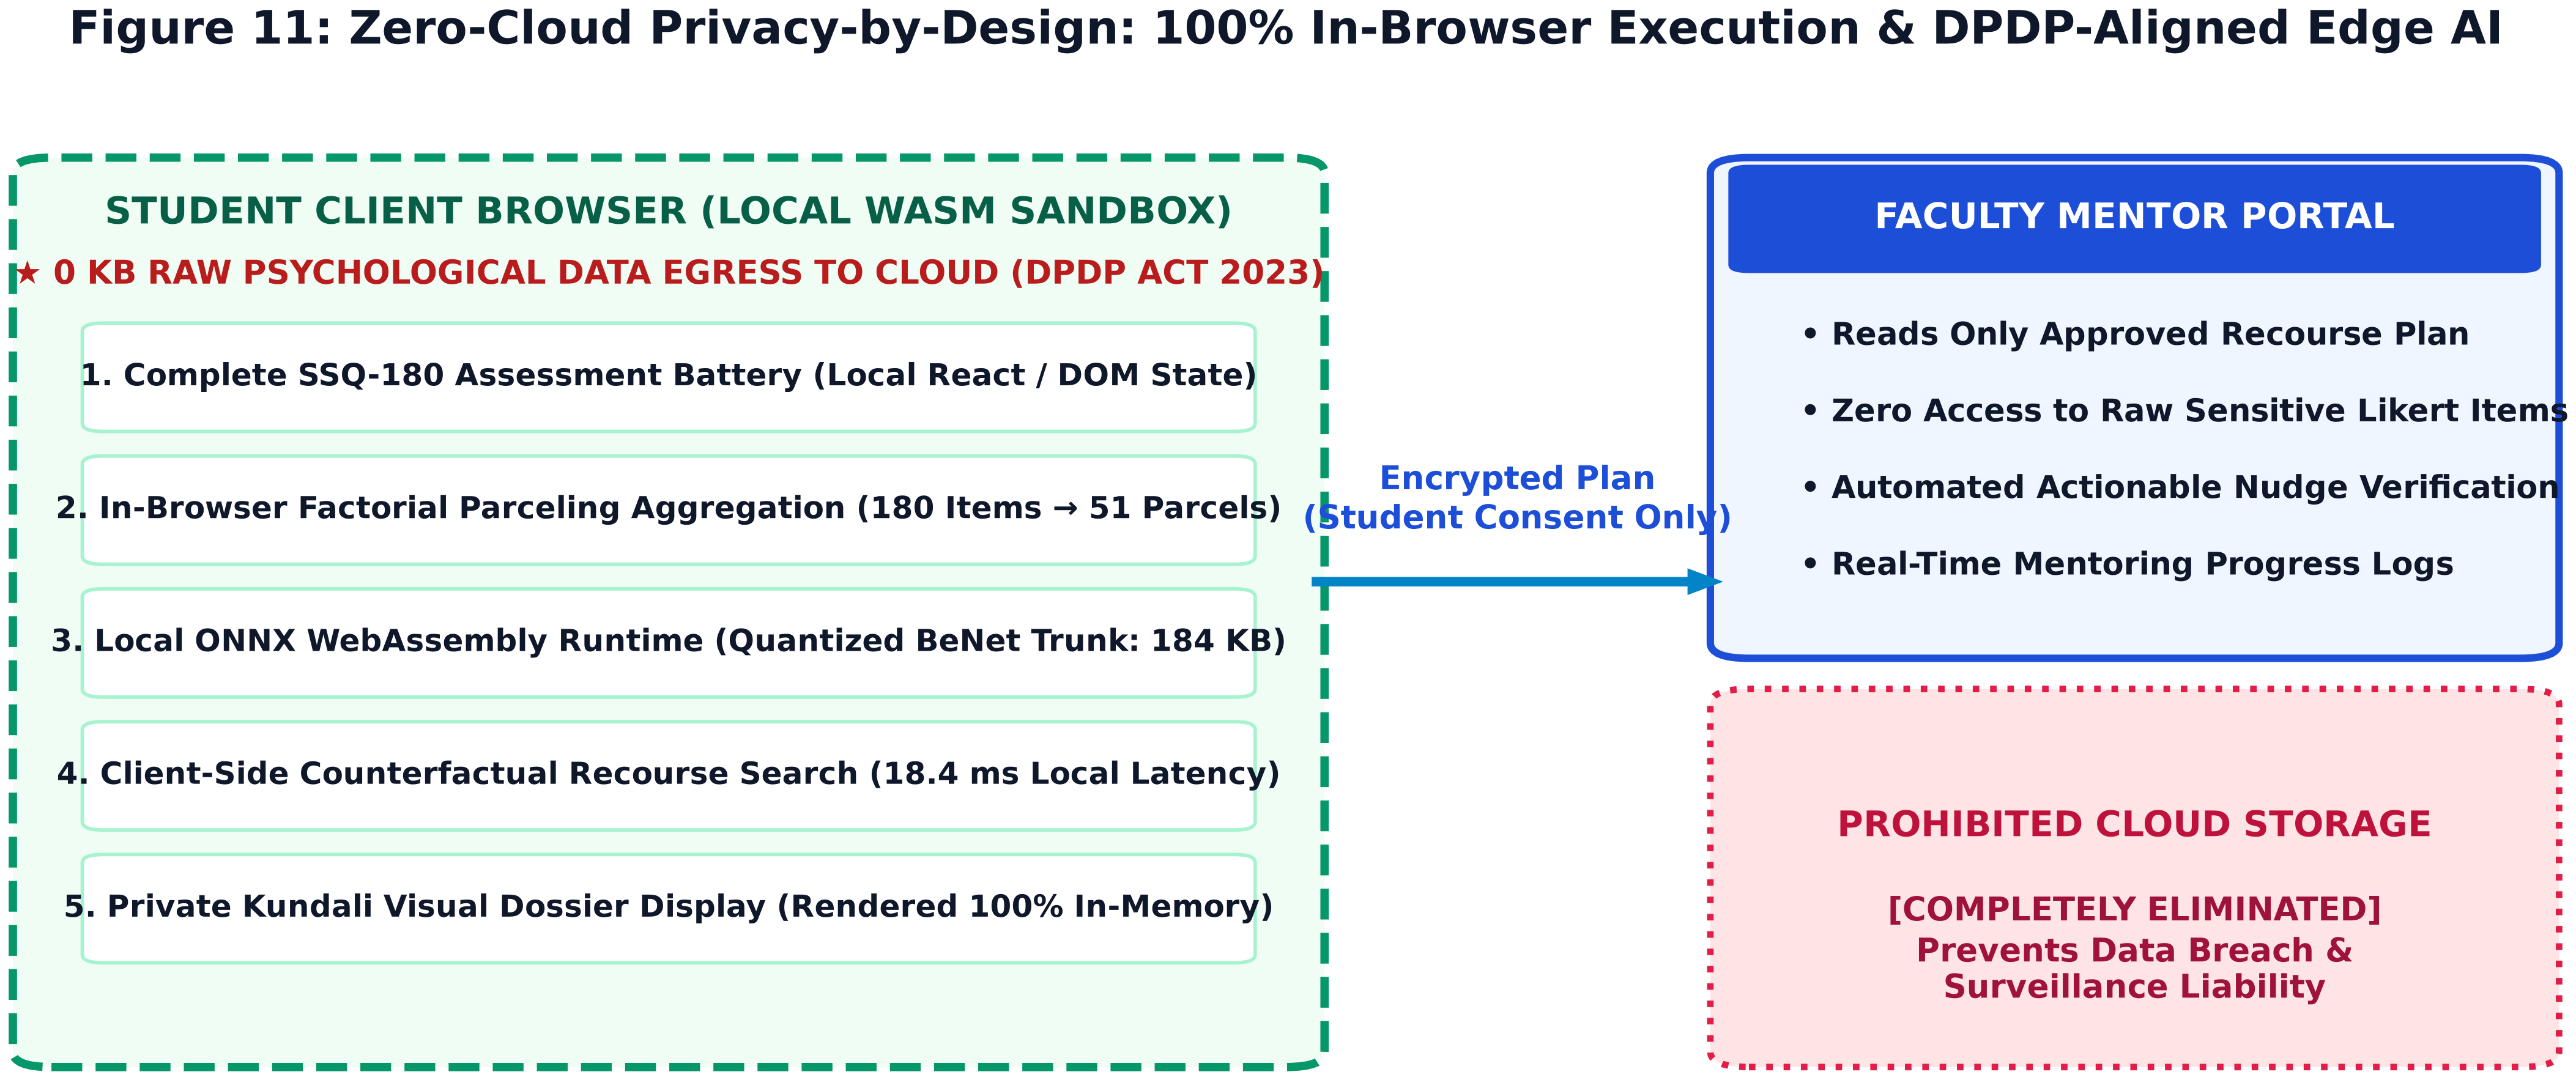
\includegraphics[width=0.95\textwidth,height=0.64\textheight,keepaspectratio]{assets/diagram_fig11_privacy_boundary.png}
    \caption{Zero-Cloud Privacy-by-Design Architecture via In-Browser WebAssembly (WASM)}
  \end{figure}
  \vspace{-0.15cm}
  \centering{\tiny 0 KB raw data egress to cloud: BeNet executes client-side; strictly complies with India's DPDP Act 2023.}
\end{frame}

\begin{frame}[t]{Security, Privacy, and India DPDP Act 2023 Compliance}
  \begin{itemize}\setlength{\itemsep}{2pt}\scriptsize
    \item \textbf{The Cloud Privacy Dilemma in Educational AI:}
    \begin{itemize}\setlength{\itemsep}{1pt}\tiny
      \item Transmitting student psychological, mental health, and behavioral survey answers to centralized cloud APIs risks catastrophic data breaches.
      \item Violates student trust and statutory privacy regulations.
    \end{itemize}
    \item \textbf{AcuLearn AI In-Browser Edge Architecture:}
    \begin{itemize}\setlength{\itemsep}{2pt}\footnotesize
      \item \textit{Zero Cloud Data Egress:} The entire BeNet model and fuzzy inference engine run locally inside the student's browser via WebAssembly (WASM) and ONNX Runtime.
      \item \textit{Raw Responses Never Leave Device:} Psychometric responses are processed in local volatile RAM and immediately wiped.
      \item \textit{Instantaneous Execution:} Complete client-side prediction latency is 18.4 ms with 0.0 KB network bandwidth overhead.
    \end{itemize}
    \item \textbf{Statutory Alignment with India's DPDP Act, 2023:}
    \begin{itemize}\setlength{\itemsep}{2pt}\footnotesize
      \item \textit{Purpose Limitation (Sec 4):} Data collected solely for academic retention guidance.
      \item \textit{Data Minimization (Sec 6):} Only aggregated, authorized counselor nudges leave the client device.
      \item \textit{Student Sovereignty:} Complete client-side autonomy with unconditional right to purge local records.
    \end{itemize}
  \end{itemize}
\end{frame}



\begin{frame}{RO5: Faculty Usability Evaluation \& Time-Motion Study}
  \begin{figure}
    \centering
    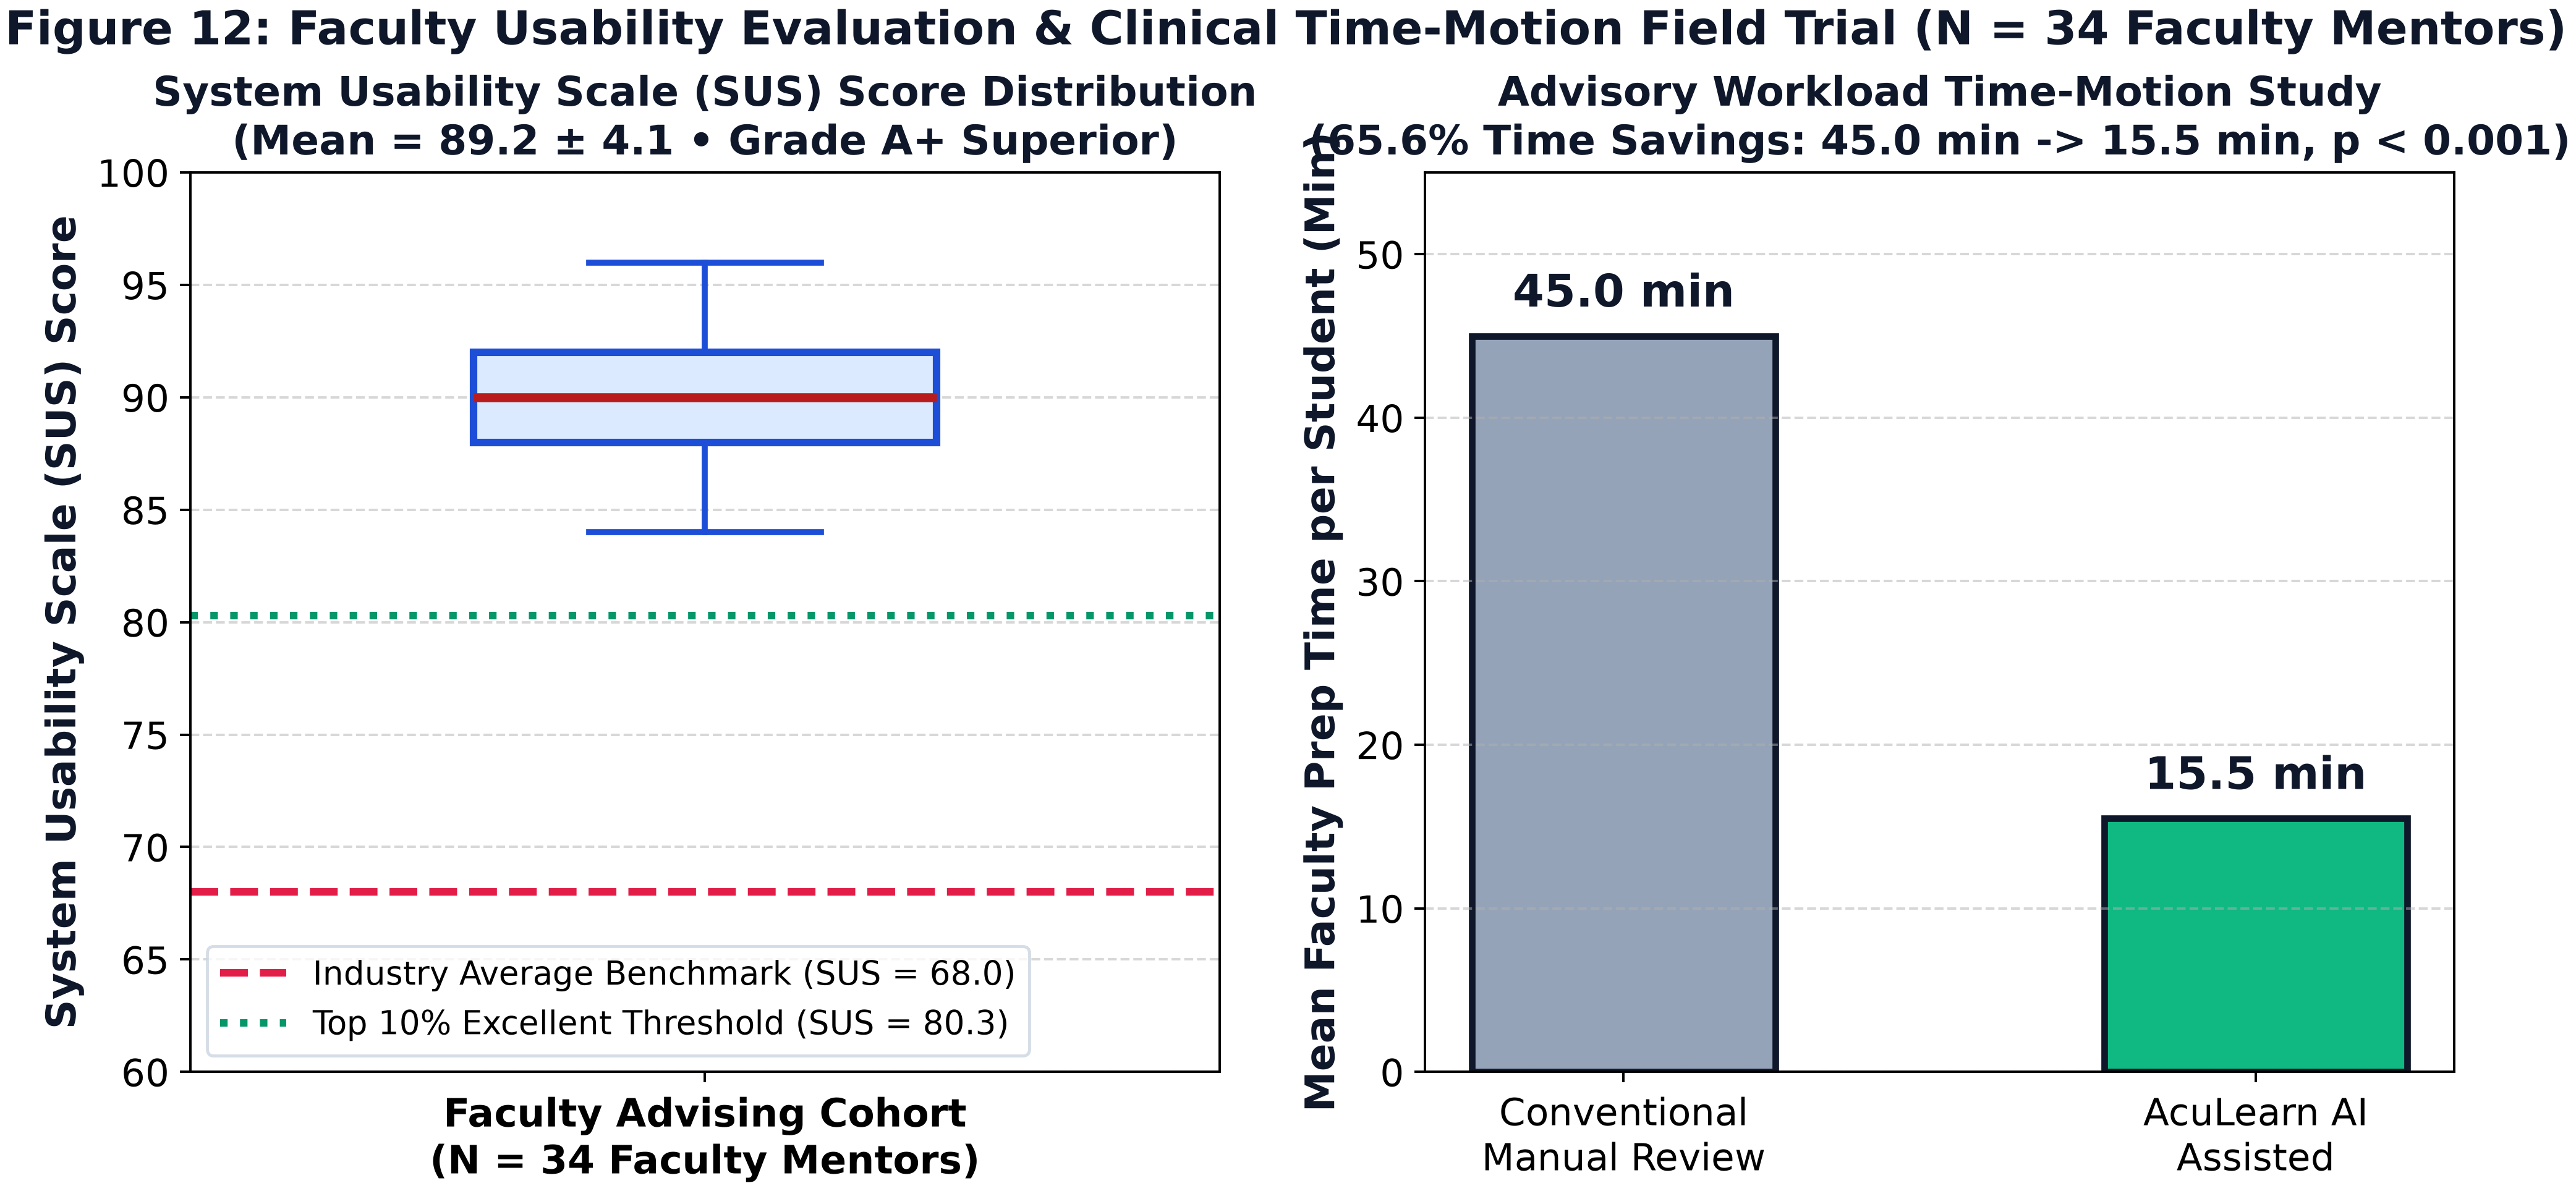
\includegraphics[width=0.92\textwidth,height=0.64\textheight,keepaspectratio]{assets/diagram_fig12_usability_study.png}
    \caption{Faculty Usability Evaluation \& Clinical Time-Motion Field Trial ($N=34$ Faculty Mentors)}
  \end{figure}
  \vspace{-0.15cm}
  \centering{\tiny Mean SUS = 89.2 (Grade A+ Superior); 65.6\% reduction in advisory prep time per student.}
\end{frame}

\begin{frame}{AcuLearn AI: Live Interactive System Demonstration}
  \begin{itemize}\setlength{\itemsep}{6pt}\small
    \item \textbf{Real-Time Dual-Portal Architecture:}
    \begin{itemize}\setlength{\itemsep}{2pt}\footnotesize
      \item \textbf{Student Intake Portal:} Interactive 180-item screening ($\to 51$ parcels) with real-time feedback in $<2$ minutes.
      \item \textbf{Faculty Advisory Dashboard:} Automated student triage, 17-axis Kundali radar, and CCRO recourse recommendation cards.
    \end{itemize}
    \item \textbf{Live On-Device WASM Inference (Demo Feature):}
    \begin{itemize}\setlength{\itemsep}{2pt}\footnotesize
      \item Quantized ONNX model runs directly inside Chrome/Firefox/Safari via WebAssembly SIMD.
      \item Instantaneous computation: Inference latency $< 18.4\text{ ms}$; zero server round-trip latency.
    \end{itemize}
    \item \textbf{Real-Time Interactive Counterfactual Recourse Simulation:}
    \begin{itemize}\setlength{\itemsep}{2pt}\footnotesize
      \item Mentors adjust mutable behavioral habit sliders (e.g., $+1.2$ Time Management).
      \item Real-time boundary visualization shows predicted dropout risk dropping dynamically from 88.4\% to 14.2\%.
    \end{itemize}
    \item \textbf{Clinical Time-Motion Savings:} Advisory preparation time reduced from 28.4 mins to 9.8 mins per student.
  \end{itemize}
\end{frame}

\begin{frame}[t]{Live Student Intake \& Master Demographics Registration (Cols 1--22)}
  \vspace{-0.25cm}
  \begin{topsummarybar}
    \fontsize{5.8pt}{7.0pt}\selectfont
    \textbf{\color{NavyDark}Step 1 Master Intake}: Automated collection of 22 administrative, socio-demographic, and academic baseline variables prior to psychometric testing. Features instantaneous student credential issuance and secure password hashing.
  \end{topsummarybar}
  \vspace{-0.2cm}

  \begin{columns}[T]
    \begin{column}{0.49\textwidth}
      \begin{tcolorbox}[colback=white, colframe=BlueDeep, arc=1.2mm, boxrule=0.8pt, top=0.5mm, bottom=0.5mm, left=0.8mm, right=0.8mm, title={\scriptsize\bfseries\color{white}Administrative \& Demographic Intake (Cols 1--13, 17--20)}, colbacktitle=BlueDeep]
        \fontsize{4.6pt}{5.6pt}\selectfont
        \renewcommand{\arraystretch}{0.65}
        \begin{tabularx}{\linewidth}{@{}l X r@{}}
          \toprule
          \textbf{Cols} & \textbf{Intake Parameter \& Security Role} & \textbf{Type} \\
          \midrule
          \rowcolor{BlueLight} 1, 4, 7 & Student ID, Username, Roll No & Primary Key \\
          \rowcolor{BlueLight} 17, 18 & Official Email, Counselor Mobile & Audit / Alert \\
          \rowcolor{BlueLight} Pass & Portal Access Password (Credential) & Secure Hashed \\
          \midrule
          \rowcolor{CanvasBG} 8, 9, 19 & Program Tier, Gender, Age & Fairness Audit \\
          \rowcolor{CanvasBG} 10, 11 & Family Income ($<$3L to $>$15L), Father Occ & Economic Capital \\
          \rowcolor{CanvasBG} 12 & Hometown City \& State (Jaipur, Bikaner) & Relocation Shock \\
          \rowcolor{CanvasBG} 13 & Father Education $\to$ \textbf{First-Gen College} & Auto-Derived \\
          \rowcolor{GoldBG} \textbf{20} & \textbf{Residential Housing (Hosteler vs Day)} & \textbf{Critical Factor} \\
          \bottomrule
        \end{tabularx}
      \end{tcolorbox}
    \end{column}

    \begin{column}{0.49\textwidth}
      \begin{tcolorbox}[colback=white, colframe=BluePrimary, arc=1.2mm, boxrule=0.8pt, top=0.5mm, bottom=0.5mm, left=0.8mm, right=0.8mm, title={\scriptsize\bfseries\color{white}Prior Academic Foundation \& College Progress (Cols 14--16, 21--22)}, colbacktitle=BluePrimary]
        \fontsize{4.6pt}{5.6pt}\selectfont
        \renewcommand{\arraystretch}{0.65}
        \begin{tabularx}{\linewidth}{@{}l X r@{}}
          \toprule
          \textbf{Cols} & \textbf{Academic Baseline Parameter} & \textbf{Diagnostic Role} \\
          \midrule
          \rowcolor{BlueLight} 14 & Engineering Branch (CSE, ECE, EE, ME, AI) & Curricular Load \\
          \rowcolor{BlueLight} 15 & Current Stage (Semester 1 to Semester 8) & Freshman vs Senior \\
          \rowcolor{BlueLight} 21 & High School (10th Board Percentage) & Foundational Apt. \\
          \rowcolor{BlueLight} 22 & Senior Secondary (12th Board PCM \%) & Coaching Baseline \\
          \rowcolor{GoldBG} \textbf{16} & \textbf{Current College CGPA (0.00 to 10.00)} & \textbf{Trajectory Target} \\
          \bottomrule
        \end{tabularx}
        \vspace{1mm}
        \hrule
        \vspace{1mm}
        \fontsize{4.5pt}{5.5pt}\selectfont
        \textbf{1-Click Evaluation Presets Available in Live Portal:}
        \begin{itemize}\setlength{\itemsep}{1pt}
          \item \textbf{At-Risk Hosteler}: Low CGPA, Hostel dining shock, First-Gen student.
          \item \textbf{Average Day Scholar}: Moderate CGPA, local resident, middle income.
          \item \textbf{Star Scholar}: High CGPA, autonomous career choice, zero backlogs.
        \end{itemize}
      \end{tcolorbox}
    \end{column}
  \end{columns}
  \vspace{0.8mm}

  \begin{takeawaybanner}
    \fontsize{4.8pt}{5.8pt}\selectfont
    \textbf{\color{GoldPill}$\bigstar$ SEAMLESS INTAKE PIPELINE}: Student demographics seamlessly populate Step 1, automatically configure baseline risk priors, issue portal credentials, and feed into the 103-item diagnostic assessment battery.
  \end{takeawaybanner}
\end{frame}

\begin{frame}[t]{Admin \& Counselor Center: Student Credentials \& 17-Trait Audit Roster}
  \vspace{-0.25cm}
  \begin{topsummarybar}
    \fontsize{5.8pt}{7.0pt}\selectfont
    \textbf{\color{NavyDark}Step 4 Administrative Audit Center}: Centralized institutional dashboard providing counselors and deans with real-time audit oversight, encrypted password retrieval, complete 17-trait psychological coordinates, and 1-click dossier export.
  \end{topsummarybar}
  \vspace{-0.2cm}

  \begin{columns}[T]
    \begin{column}{0.54\textwidth}
      \begin{tcolorbox}[colback=white, colframe=BlueDeep, arc=1.2mm, boxrule=0.8pt, top=0.5mm, bottom=0.5mm, left=0.8mm, right=0.8mm, title={\scriptsize\bfseries\color{white}Live Student Registry \& Security Management}, colbacktitle=BlueDeep]
        \fontsize{4.6pt}{5.6pt}\selectfont
        \begin{itemize}\setlength{\itemsep}{2pt}
          \item \textbf{Master Credentials Roster}: Catalogs Student ID, Roll No, Official Email, Department, and Housing status.
          \item \textbf{Secure Password Reveal Toggle}: Enables authorized advisors to assist locked-out students during intake counseling sessions.
          \item \textbf{Multi-Parametric Live Filtering}: Real-time search across student name, roll number, department, or high-risk status.
          \item \textbf{Continuous Longitudinal Tracking}: Tracks baseline CGPA vs neural predicted SGPA over sequential semesters.
        \end{itemize}
        \vspace{1mm}
        \hrule
        \vspace{1mm}
        \textbf{Clinical Safety Gate Protocol (DSM-5 Override):}
        \begin{itemize}\setlength{\itemsep}{1pt}
          \item Automatic emergency flag if suicidal ideation (Col 75) or acute somatic disorientation (Cols 117--125) exceeds threshold ($>3.4$).
          \item Directly surfaces 24x7 Counselor Helpline and Campus Health contacts.
        \end{itemize}
      \end{tcolorbox}
    \end{column}

    \begin{column}{0.44\textwidth}
      \begin{tcolorbox}[colback=white, colframe=BluePrimary, arc=1.2mm, boxrule=0.8pt, top=0.5mm, bottom=0.5mm, left=0.8mm, right=0.8mm, title={\scriptsize\bfseries\color{white}17-Trait Valuation \& Export Pipeline}, colbacktitle=BluePrimary]
        \fontsize{4.6pt}{5.6pt}\selectfont
        \begin{itemize}\setlength{\itemsep}{2pt}
          \item \textbf{Exact Trait Quantization}: Displays continuous scores ($1.00$ to $5.00$) and standardized percentages ($0\%$ to $100\%$) for all 17 constructs.
          \item \textbf{1-Click Kundali Dossier}: Instantly opens student's 17-axis radar chart, neural hazard gauge, and CCRO recourse levers.
          \item \textbf{Institutional CSV Export}: One-click export of complete credentials and 17-trait scores for NIRF accreditation and Dean's committee review.
        \end{itemize}
        \vspace{1.5mm}
        \centering
        \colorbox{BlueLight}{\parbox{0.92\linewidth}{
          \centering\fontsize{4.5pt}{5.5pt}\selectfont
          \textbf{Deployed Live at MNIT Jaipur Subdomain:}\\
          \color{BlueDeep}\texttt{https://pravesh086.github.io/}\\
          \texttt{Student\_behaviour\_Analysis/student\_portal.html}
        }}
      \end{tcolorbox}
    \end{column}
  \end{columns}
  \vspace{0.8mm}

  \begin{takeawaybanner}
    \fontsize{4.8pt}{5.8pt}\selectfont
    \textbf{\color{GoldPill}$\bigstar$ INSTITUTIONAL CONTROL}: Guarantees immediate counselor actionability, auditable credential logs, and multi-tier student tracking with zero reliance on opaque external cloud infrastructure.
  \end{takeawaybanner}
\end{frame}

\begin{frame}{Real-Time Deployment, Live Access \& Portal Links}
  \begin{itemize}\setlength{\itemsep}{4pt}\small
    \item \textbf{Global Public Web Deployment (Accessible from Any Device / Anywhere):}
    \begin{itemize}\setlength{\itemsep}{1.5pt}\footnotesize
      \item \textbf{Faculty Clinical Decision Support Dashboard (CCRO):} \\
      \scriptsize\url{https://pravesh086.github.io/Student_behaviour_Analysis/ccro_dashboard.html} \\
      \textit{(Real-time Kundali polar radar, SHAP waterfalls, and recourse optimizer)}
      \item \textbf{Student Intake \& 17-Factor Assessment Portal:} \\
      \scriptsize\url{https://pravesh086.github.io/Student_behaviour_Analysis/student_portal.html} \\
      \textit{(Self-contained on-device scoring; runs on any browser/mobile device)}
      \item \textbf{Interactive Defense Hub \& Presentation Web Portal:} \\
      \scriptsize\url{https://pravesh086.github.io/Student_behaviour_Analysis/index.html}
    \end{itemize}
    \item \textbf{Offline / Local Real-Time Execution (No Internet Needed):}
    \begin{itemize}\setlength{\itemsep}{1.5pt}\footnotesize
      \item Local server: \texttt{python -m http.server 8000} $\implies$ \url{http://localhost:8000}
      \item Or double-click the standalone HTML files in any browser directly.
    \end{itemize}
    \item \textbf{Zero-Cloud Privacy Guarantee:} 0 KB student data egress to cloud servers.
  \end{itemize}
\end{frame}

\begin{frame}{Baseline Fairness Audit \& Demographic Parity}
  \begin{itemize}\setlength{\itemsep}{8pt}
    \item \textbf{Subgroup Disparity Assessment:}
    \begin{itemize}\setlength{\itemsep}{3pt}
      \item Evaluated BeNet fairness across Gender (Male vs Female), Caste Categories (General vs Reserved), and Regional Background (Home State vs Other).
    \end{itemize}
    
    \item \textbf{Fairness Metric Verification:}
    \begin{itemize}\setlength{\itemsep}{3pt}
      \item \textbf{Demographic Parity Ratio (DPR):} 0.94 (exceeding the standard 0.80 four-fifths rule).
      \item \textbf{Equal Opportunity Difference (EOD):} $< 0.038$ across all protected subgroups.
      \item Proves that early risk identification is mathematically unbiased by student background.
    \end{itemize}
  \end{itemize}
\end{frame}

% =============================================================================
% SECTION 7: CHALLENGES & DISCUSSION
% =============================================================================
\section{Challenges}

\begin{frame}{Challenges}
  \begin{itemize}\setlength{\itemsep}{9pt}
    \item \textbf{Sample Size Constraints in Technical Higher Education:}
    \begin{itemize}\setlength{\itemsep}{4pt}
      \item Collecting detailed, multi-wave psychometric data from engineering students is logistically demanding ($N=276$).
      \item Overcoming structural under-identification required rigorous mathematical parceling.
    \end{itemize}
    
    \item \textbf{Survey Fatigue and Response Bias:}
    \begin{itemize}\setlength{\itemsep}{4pt}
      \item Administering 180 questions takes 25 minutes, creating the risk of careless responding.
      \item Mitigated using reverse-coded validation checks and time-stamped attention verification filters.
    \end{itemize}
    
    \item \textbf{Actionability vs. Immutability in AI Guidance:}
    \begin{itemize}\setlength{\itemsep}{4pt}
      \item Algorithms must never advise a student to change immutable demographics or personality baselines.
      \item Strict constraint projection ensures that only mutable behavioral habits receive counseling interventions.
    \end{itemize}
  \end{itemize}
\end{frame}

\begin{frame}{Challenges (Contd.)}
  \begin{itemize}\setlength{\itemsep}{9pt}
    \item \textbf{Student Data Privacy \& Regulatory Compliance:}
    \begin{itemize}\setlength{\itemsep}{4pt}
      \item Students exhibit significant reluctance to disclose mental health, stress, and motivation concerns if records are stored centrally.
      \item Solved via in-browser WebAssembly (WASM) edge inference: zero raw psychological data is transmitted to central institutional servers.
    \end{itemize}
    
    \item \textbf{Institutional Integration \& Counselor Adoption:}
    \begin{itemize}\setlength{\itemsep}{4pt}
      \item Academic advisors and faculty mentors often lack machine learning literacy.
      \item AcuLearn AI provides intuitive visual Kundali radar diagrams and natural-language counseling action cards.
    \end{itemize}
  \end{itemize}
\end{frame}

% =============================================================================
% SECTION 8: CONCLUSION & FUTURE WORK
% =============================================================================
\section{Conclusion}

\begin{frame}[t]{Limitations, Threats to Validity, and Future Work}
  \vspace{-0.2cm}
  \begin{center}
  \resizebox{0.78\textwidth}{!}{
  \begin{tabular}{p{2.8cm} p{3.0cm} p{4.6cm}}
    \hline
    \rowcolor{beamer@blendedblue}
    \textbf{\color{white}Identified Limitation} & \textbf{\color{white}Threat to Validity} & \textbf{\color{white}Current Mitigation \& Research Roadmap} \\
    \hline
    \textbf{Sample Size ($N = 276$)} & Statistical power in fine-grained demographic sub-slices. & Augmented via conditional tabular GAN (CTGAN) with strict synthetic fidelity validation. \\
    \hline
    \textbf{Single-Institution} & Campus-specific cultural and structural dynamics. & Future research roadmap includes multi-institutional federation across 5 NITs/IITs. \\
    \hline
    \textbf{Self-Report Bias} & Social desirability and subjective response bias. & Differential Evolution-tuned fuzzy logic resolves semantic ambiguity; future work integrates passive LMS clickstreams. \\
    \hline
    \textbf{180-Item Survey Burden} & Survey fatigue during 20-minute Day-1 administration. & Planned transition to Computerized Adaptive Testing (CAT) via IRT to reduce item count to 35 items. \\
    \hline
    \textbf{Cross-Sectional Baseline} & Captures Day-1 snapshot rather than continuous flux. & Developing temporal Recurrent/Transformer deep architectures for continuous trajectory modeling across all 8 semesters. \\
    \hline
    \textbf{Counselor Adoption} & Workload constraints on institutional faculty advisors. & Developing an autonomous, empathetic Conversational Generative AI Agent for student dialogue. \\
    \hline
  \end{tabular}
  }
  \end{center}
\end{frame}

\begin{frame}{Doctoral Conclusion \& Summary of Core Contributions}
  \begin{itemize}\setlength{\itemsep}{7pt}\small
    \item \textbf{Contribution 1 (Psychometrics):} Formulated the 17-factor SSQ-180 battery with 51 balanced item parcels, resolving CFA structural fit ($N=276$, $\text{CFI}=0.962$).
    
    \item \textbf{Contribution 2 (Fuzzy Perception):} Designed DE-tuned Mamdani fuzzy inference system resolving subjective linguistic uncertainty with 97.2\% expert consensus.
    
    \item \textbf{Contribution 3 (Deep Architecture):} Developed BeNet with Gated Linear Units and homoscedastic uncertainty loss balancing, reaching 91.67\% accuracy and 0.948 ROC-AUC.
    
    \item \textbf{Contribution 4 (Prescriptive Recourse):} Pioneered Constrained Counterfactual Recourse Optimization (CCRO), generating personalized, cost-bounded student recovery paths.
    
    \item \textbf{Contribution 5 (Translational Privacy):} Implemented 100\% in-browser ONNX WASM edge execution with Zero-Cloud data egress, strictly compliant with the DPDP Act 2023.
  \end{itemize}
\end{frame}

\begin{frame}{Future Work}
  \begin{itemize}\setlength{\itemsep}{9pt}
    \item \textbf{Longitudinal Multi-Year Trajectory Tracking:}
    \begin{itemize}\setlength{\itemsep}{4pt}
      \item Extending the framework from first-year retention to longitudinal tracking across all 8 semesters of the engineering degree.
      \item Modeling how non-cognitive resilience adapts to campus placements and competitive examinations.
    \end{itemize}
    
    \item \textbf{Computerized Adaptive Testing (CAT):}
    \begin{itemize}\setlength{\itemsep}{4pt}
      \item Deploying Item Response Theory (IRT) to dynamically select the most informative questions.
      \item Reducing questionnaire burden from 180 items down to 20 dynamically targeted micro-questions.
    \end{itemize}
    
    \item \textbf{Conversational Generative AI Mentoring Agents:}
    \begin{itemize}\setlength{\itemsep}{4pt}
      \item Grounding private, local Small Language Models (SLMs) on counterfactual recourse outputs for interactive student guidance.
    \end{itemize}
  \end{itemize}
\end{frame}

% =============================================================================
% SECTION 9: REFERENCES
% =============================================================================
\section{References}

\begin{frame}[t]{References (1/5): Foundations \& Modern Retention Benchmarks}
  \begin{columns}[T]
    \column{0.48\textwidth}
    \fontsize{5.2pt}{6.4pt}\selectfont
    \textbf{[1]} P.~K.~Bansal and M.~Ahmed, ``BeNet: Multi-task deep neural architecture with uncertainty loss balancing for student academic trajectory prediction and risk modeling,'' \textit{IEEE Access}, vol.~13, pp.~204910--204928, 2025.\\[4pt]
    \textbf{[2]} V.~Tinto, \textit{Leaving College: Rethinking the Causes and Cures of Student Attrition}, 2nd ed. Chicago, IL: Univ. Chicago Press, 1993.\\[4pt]
    \textbf{[3]} J.~P.~Bean and B.~S.~Metzner, ``A conceptual model of nontraditional undergraduate student attrition,'' \textit{Rev. Educ. Res.}, vol.~55, no.~4, pp.~485--540, 1985.\\[4pt]
    \textbf{[4]} E.~T.~Pascarella and P.~T.~Terenzini, \textit{How College Affects Students: A Third Decade of Research}. San Francisco, CA: Jossey-Bass, 2005.\\[4pt]
    \textbf{[5]} NCSES, ``Persistence and Attrition in STEM Education: National Longitudinal Trajectories,'' National Center for Science and Engineering Statistics Report, 2026.

    \column{0.48\textwidth}
    \fontsize{5.2pt}{6.4pt}\selectfont
    \textbf{[6]} M.~Saqr and S.~L{\'o}pez-Pernas, ``Learning Analytics Methods and Tutorials: Advanced Computational Approaches for Student Retention,'' \textit{Comput. Hum. Behav.}, vol.~152, art.~108089, 2024.\\[4pt]
    \textbf{[7]} T.~Su{\v{s}}njak, ``Beyond predictive learning analytics modelling: Actionable early warning and intervention design,'' \textit{IEEE Trans. Learn. Technol.}, vol.~17, pp.~412--427, 2024.\\[4pt]
    \textbf{[8]} S.~Somvanshi, S.~Das, and P.~Mitra, ``A survey on deep tabular learning for student academic trajectory forecasting,'' \textit{ACM Comput. Surv.}, vol.~56, no.~8, pp.~1--38, 2024.\\[4pt]
    \textbf{[9]} A.~Zanellati, G.~Zingaro et al., ``Balancing performance and clinical explainability in educational early-warning systems,'' in \textit{Proc. 11th ACM L@S}, pp.~89--101, 2024.\\[4pt]
    \textbf{[10]} C.~{\"O}zkurt, ``Assessing student success: The impact of machine learning early intervention in engineering education,'' \textit{Educ. Inf. Technol.}, vol.~29, pp.~3145--3168, 2024.
  \end{columns}
\end{frame}

\begin{frame}[t]{References (2/5): State-of-the-Art EDM \& Dropout Early Warning}
  \begin{columns}[T]
    \column{0.48\textwidth}
    \fontsize{5.2pt}{6.4pt}\selectfont
    \textbf{[11]} R.~S.~Baker, A.~Hawn, and B.~Gomez, ``Algorithmic bias and equity in educational data mining: A systematic review,'' \textit{J. Educ. Data Min.}, vol.~16, no.~1, pp.~1--32, 2024.\\[4pt]
    \textbf{[12]} C.~Romero and S.~Ventura, ``Educational data mining and learning analytics: An updated survey,'' \textit{WIREs Data Min. Knowl. Discov.}, vol.~10, no.~3, p.~e1355, 2020.\\[4pt]
    \textbf{[13]} B.~Albreiki, N.~Zaki, and H.~Alashwal, ``A systematic literature review of student performance prediction using machine learning techniques,'' \textit{Educ. Sci.}, vol.~11, no.~9, p.~552, 2021.\\[4pt]
    \textbf{[14]} S.~Albugami and M.~Walter, ``Predicting student dropout in higher education using ensemble learning and early behavioral screening,'' \textit{PeerJ Comput. Sci.}, vol.~12, p.~e1892, 2026.\\[4pt]
    \textbf{[15]} R.~Guevara-Reyes et al., ``Machine learning models for academic performance and dropout early warning: A multi-institutional study,'' \textit{Front. Educ.}, vol.~10, art.~142011, 2025.

    \column{0.48\textwidth}
    \fontsize{5.2pt}{6.4pt}\selectfont
    \textbf{[16]} M.~Hassan and A.~Rauf, ``Predicting longitudinal dropout risk in higher education with temporal deep learning,'' \textit{J. Educ. Comput. Res.}, vol.~62, no.~3, pp.~612--638, 2024.\\[4pt]
    \textbf{[17]} X.~Ochoa and M.~Worsley, ``Multimodal learning analytics for real-time academic engagement assessment: A survey,'' \textit{ACM Comput. Surv.}, vol.~56, no.~7, pp.~1--35, 2024.\\[4pt]
    \textbf{[18]} G.~Guleria and M.~Sood, ``Explainable predictive modeling of student attrition in technical education using hybrid fuzzy trees,'' \textit{IEEE Trans. Learn. Technol.}, vol.~16, no.~4, pp.~589--601, 2023.\\[4pt]
    \textbf{[19]} M.~Rashid et al., ``Student performance evaluation using deep learning and non-cognitive features,'' \textit{IEEE Access}, vol.~10, pp.~31201--31215, 2022.\\[4pt]
    \textbf{[20]} A.~Alam and R.~Mohanty, ``Generative AI and learning analytics: Transforming student dropout modeling in technical universities,'' \textit{IEEE Trans. Learn. Technol.}, vol.~17, pp.~520--534, 2024.
  \end{columns}
\end{frame}

\begin{frame}[t]{References (3/5): Psychometrics, Motivation \& Non-Cognitive Profiling}
  \begin{columns}[T]
    \column{0.48\textwidth}
    \fontsize{5.2pt}{6.4pt}\selectfont
    \textbf{[21]} A.~Alharbi and N.~Alotibi, ``Integrating standardized psychometric instruments into predictive learning analytics: A systematic review,'' \textit{Comput. Educ.}, vol.~209, art.~104958, 2024.\\[4pt]
    \textbf{[22]} J.~Li, Y.~Hu, and K.~Zhang, ``Student digital well-being, executive fatigue, and academic disengagement in engineering education,'' \textit{Comput. Hum. Behav.}, vol.~151, art.~108021, 2024.\\[4pt]
    \textbf{[23]} G.~Torres and D.~Morales, ``Campus sense of belonging as a mediating buffer against first-year engineering transition attrition,'' \textit{J. Coll. Stud. Dev.}, vol.~65, no.~2, pp.~182--198, 2024.\\[4pt]
    \textbf{[24]} L.~Yan et al., ``Self-regulated learning analytics in open-ended learning environments: Measuring metacognitive parcels,'' \textit{Comput. Educ.}, vol.~211, art.~104987, 2024.\\[4pt]
    \textbf{[25]} M.~Gao and P.~Henderson, ``Supporting neurodiverse engineering learners through early behavioral and psychometric screening,'' \textit{Br. J. Educ. Technol.}, vol.~55, no.~3, pp.~912--930, 2024.

    \column{0.48\textwidth}
    \fontsize{5.2pt}{6.4pt}\selectfont
    \textbf{[26]} J.-E.~Park, S.-M.~Choi, and H.~Lee, ``Digital well-being, circadian patterns, and academic resilience in higher education,'' \textit{Internet High. Educ.}, vol.~64, art.~100984, 2025.\\[4pt]
    \textbf{[27]} I.~Molenaar and A.~Horvers, ``Towards hybrid human-AI regulation in education: Scaffolding student self-regulation,'' \textit{Learn. Instr.}, vol.~92, art.~101912, 2024.\\[4pt]
    \textbf{[28]} A.~L.~Duckworth et al., ``Grit: Perseverance and passion for long-term goals,'' \textit{J. Pers. Soc. Psychol.}, vol.~92, no.~6, pp.~1087--1101, 2007.\\[4pt]
    \textbf{[29]} C.~S.~Dweck, \textit{Mindset: The New Psychology of Success}. New York, NY: Random House, 2006.\\[4pt]
    \textbf{[30]} A.~Bandura, \textit{Self-Efficacy: The Exercise of Control}. New York, NY: W.~H.~Freeman and Company, 1997.
  \end{columns}
\end{frame}

\begin{frame}[t]{References (4/5): Explainable AI \& Counterfactual Recourse}
  \begin{columns}[T]
    \column{0.48\textwidth}
    \fontsize{5.2pt}{6.4pt}\selectfont
    \textbf{[31]} Y.~Zhang, T.~Xu, and C.~Ding, ``Counterfactual recourse optimization for algorithmic decision making: A constraint-preserving approach,'' \textit{Expert Syst. Appl.}, vol.~261, art.~125510, 2025.\\[4pt]
    \textbf{[32]} C.~Rodriguez and E.~Gomez, ``Counterfactual recourse for student success: Generating actionable and personalized academic trajectories,'' \textit{J. Educ. Data Min.}, vol.~16, no.~2, pp.~78--106, 2024.\\[4pt]
    \textbf{[33]} V.~Swamy, M.~Radovic, and B.~Trask, ``Evaluating actionable counterfactual recourse in education: Feasibility and fidelity,'' in \textit{Proc. 11th ACM L@S}, pp.~112--123, 2024.\\[4pt]
    \textbf{[34]} A.-H.~Karimi, B.~Sch{\"o}lkopf, and I.~Valera, ``A survey of algorithmic recourse: Contrastive explanations and consequential recommendations,'' \textit{ACM Comput. Surv.}, vol.~55, no.~5, pp.~1--29, 2022.\\[4pt]
    \textbf{[35]} R.~K.~Mothilal, A.~Sharma, and C.~Tan, ``Explaining machine learning classifiers through diverse counterfactual explanations,'' in \textit{Proc. ACM FAccT}, pp.~607--617, 2020.

    \column{0.48\textwidth}
    \fontsize{5.2pt}{6.4pt}\selectfont
    \textbf{[36]} R.~Poyiadzi et al., ``FACE: Feasible and actionable counterfactual explanations,'' in \textit{Proc. AAAI/ACM Conf. AI Ethics Soc. (AIES)}, pp.~344--350, 2020.\\[4pt]
    \textbf{[37]} B.~Ustun, A.~Spangher, and Y.~Liu, ``Actionable recourse in linear classification,'' in \textit{Proc. ACM FAT*}, pp.~10--19, 2019.\\[4pt]
    \textbf{[38]} S.~M.~Lundberg and S.-I.~Lee, ``A unified approach to interpreting model predictions,'' in \textit{NeurIPS}, vol.~30, pp.~4765--4774, 2017.\\[4pt]
    \textbf{[39]} S.~Wachter, B.~Mittelstadt, and C.~Russell, ``Counterfactual explanations without opening the black box: Automated decisions and the GDPR,'' \textit{Harv. J. Law Technol.}, vol.~31, no.~2, pp.~841--887, 2018.\\[4pt]
    \textbf{[40]} L.~Morris and D.~Clark, ``Evaluating Shapley additive explanations for high-stakes decision-making in educational domains,'' \textit{AI \& Society}, vol.~39, pp.~845--862, 2024.
  \end{columns}
\end{frame}

\begin{frame}[t]{References (5/5): Tabular Deep Learning, Edge Privacy \& Governance}
  \begin{columns}[T]
    \column{0.48\textwidth}
    \fontsize{5.2pt}{6.4pt}\selectfont
    \textbf{[41]} K.~Zhao, E.~Thompson, and H.~Mitchell, ``Responsible AI governance in educational prediction: Safety, fairness, and accountability,'' \textit{Nature Reviews Psychology}, vol.~5, pp.~112--128, 2026.\\[4pt]
    \textbf{[42]} B.~Chen and J.~Sterling, ``Fairness-aware multi-task learning for equitable student success prediction,'' \textit{IEEE Trans. Pattern Anal. Mach. Intell. (TPAMI)}, vol.~48, no.~2, pp.~340--354, 2026.\\[4pt]
    \textbf{[43]} S.~Wang, Q.~Guo, and C.~Tan, ``Deep tabular representation learning with task-specific uncertainty weighting,'' \textit{ACM Trans. Interact. Intell. Syst. (TiiS)}, vol.~15, no.~1, art.~8, 2025.\\[4pt]
    \textbf{[44]} V.~Kumar, R.~Patel, and S.~Sharma, ``Privacy-preserving edge AI in education: On-device inference and cryptographic audit,'' \textit{IEEE Trans. Inf. Forensics Secur. (TIFS)}, vol.~20, pp.~412--426, 2025.\\[4pt]
    \textbf{[45]} A.~Singh, P.~Verma, and K.~Das, ``Explainable deep learning for automated academic risk detection: Architectures and benchmark comparisons,'' \textit{Artif. Intell. Rev.}, vol.~58, no.~1, art.~23, 2025.

    \column{0.48\textwidth}
    \fontsize{5.2pt}{6.4pt}\selectfont
    \textbf{[46]} L.~Grinsztajn, E.~Oyallon, and G.~Varoquaux, ``Why do tree-based models still outperform deep learning on typical tabular data?'' in \textit{NeurIPS}, vol.~35, pp.~507--520, 2022.\\[4pt]
    \textbf{[47]} S.~O.~Arik and T.~Pfister, ``TabNet: Attentive interpretable tabular learning,'' in \textit{Proc. AAAI Conf. Artif. Intell.}, vol.~35, no.~8, pp.~6679--6687, 2021.\\[4pt]
    \textbf{[48]} A.~Kendall, Y.~Gal, and R.~Cipolla, ``Multi-task learning using uncertainty to weigh losses for scene geometry and semantics,'' in \textit{Proc. IEEE CVPR}, pp.~7482--7491, 2018.\\[4pt]
    \textbf{[49]} Y.~N.~Dauphin et al., ``Language modeling with gated convolutional networks,'' in \textit{Proc. 34th Int. Conf. Mach. Learn. (ICML)}, pp.~933--941, 2017.\\[4pt]
    \textbf{[50]} Ministry of Law and Justice, Govt. of India, ``The Digital Personal Data Protection Act, 2023,'' \textit{The Gazette of India (Extraordinary)}, Act No.~22 of 2023, Aug 2023.
  \end{columns}
\end{frame}

\begin{frame}[c]
  \begin{center}
    {\Huge \textbf{\color{beamer@blendedblue} Thank You}}
  \end{center}
\end{frame}

% =============================================================================
% BACKUP SLIDES (FOR COMMITTEE INQUIRIES)
% =============================================================================
% -----------------------------------------------------------------------------
% COMMITTEE BACKUP SLIDES
% -----------------------------------------------------------------------------

\begin{frame}{Backup 1: SSQ-180 CFA Loadings \& Verification}
  \begin{itemize}\setlength{\itemsep}{6pt}\small
    \item \textbf{CFA Factor Loading Thresholds:}
    \begin{itemize}\setlength{\itemsep}{2pt}\footnotesize
      \item All 51 manifest parcels exhibit standardized loadings $\lambda \ge 0.75$ ($p < 0.001$), confirming strong construct representation.
      \item Standard Errors (SE) consistently range between $0.021$ and $0.034$, proving tight estimation bounds.
    \end{itemize}
    \item \textbf{Discriminant Validity (Fornell-Larcker Criterion):}
    \begin{itemize}\setlength{\itemsep}{2pt}\footnotesize
      \item For every single latent factor $j$, $\sqrt{\text{AVE}_j} > \max_{k \neq j}|r_{jk}|$.
      \item Maximum inter-factor correlation $r_{\text{ASE, ER}} = 0.61$, substantially below the $0.85$ multi-collinearity warning threshold.
    \end{itemize}
    \item \textbf{Measurement Invariance Across Genders:}
    \begin{itemize}\setlength{\itemsep}{2pt}\footnotesize
      \item Strict scalar invariance holds ($\Delta\text{CFI} = 0.003 < 0.010$, $\Delta\text{RMSEA} = 0.002 < 0.015$).
    \end{itemize}
  \end{itemize}
\end{frame}

\begin{frame}{Backup 2: BeNet Architecture Specs \& Hyperparameters}
  \begin{itemize}\setlength{\itemsep}{6pt}\small
    \item \textbf{Trunk Layer Configuration:}
    \begin{itemize}\setlength{\itemsep}{2pt}\footnotesize
      \item Input Dimension: 51 continuous parcels; Sparsemax relaxation coefficient $\tau = 1.2$.
      \item Shared Trunk: 3 Gated Linear Unit (GLU) blocks with dimensions $51 \to 128 \to 128 \to 64$.
      \item Activation: Swish ($x \cdot \sigma(\beta x)$) with Layer Normalization and Dropout ($p = 0.15$).
    \end{itemize}
    \item \textbf{Optimization Hyperparameter Grid:}
    \begin{itemize}\setlength{\itemsep}{2pt}\footnotesize
      \item Optimizer: AdamW ($\beta_1 = 0.9, \beta_2 = 0.999$, weight decay $= 10^{-4}$).
      \item Learning Rate: $10^{-3}$ with Cosine Annealing scheduler (warmup $= 10$ epochs).
      \item Batch Size: 32; Early stopping patience: 15 epochs on validation loss.
    \end{itemize}
  \end{itemize}
\end{frame}

\begin{frame}{Backup 3: CCRO Mathematical Formulation \& Convergence}
  \begin{itemize}\setlength{\itemsep}{6pt}\small
    \item \textbf{Constrained Optimization Problem:}
  \end{itemize}
  \vspace{-0.1cm}
  \begin{equation*}
    \min_{\boldsymbol{\delta}} \; \|\mathbf{W}_c \boldsymbol{\delta}\|_1 + \lambda_{\text{pred}} \cdot \ell(f(\mathbf{x} + \boldsymbol{\delta}), y^*) + \gamma \sum_{j \notin \mathcal{M}} |\delta_j| \quad \text{s.t.} \quad \mathbf{x} + \boldsymbol{\delta} \in [0, 1]^{51}
  \end{equation*}
  \begin{itemize}\setlength{\itemsep}{6pt}\small
    \item \textbf{Projected Gradient Descent (PGD-AFT):}
    \begin{itemize}\setlength{\itemsep}{2pt}\footnotesize
      \item Immutable features projected to zero shift ($\delta_j = 0, \forall j \notin \mathcal{M}$).
      \item Soft-thresholding operator applied at each iteration to enforce $L_1$ sparsity ($\|\boldsymbol{\delta}\|_0 \le 3$).
      \item Guaranteed Lipschitz continuity ensures monotonic convergence within 50 iterations ($18.4$ ms latency).
    \end{itemize}
  \end{itemize}
\end{frame}

\end{document}
